
\subsection{JavaScript versus Data Science}\label{s:en}

We were going to call this book \emph{JavaScript for Scientists and
Engineers}, but \href{https://www.dabeaz.com/}{David Beazley} thought
that ``versus'' would make a better title. That one-word change sums up
how many people view the language, but we hope we can convince you that
modern JavaScript is usable as well as useful. We changed the second
half of the title because hey, data science. We also hope that these
lessons will help librarians, digital humanists, and everyone else who
uses computing in their research, not just scientists and engineers.

We will cover:

\begin{itemize}
\tightlist
\item
  Core features of modern JavaScript
\item
  Programming with callbacks and promises
\item
  Creating objects and classes
\item
  Writing HTML and CSS
\item
  Creating interactive pages with React
\item
  Building data services
\item
  Testing
\item
  Data visualization
\item
  Combining everything to create a three-tier web application
\end{itemize}

\subsubsection{Intended Audience}\label{s:intro-audience}

We assume that you:

\begin{itemize}
\tightlist
\item
  can write two-page programs that use lists, loops, conditionals, and
  functions,
\item
  can run commands in the Unix shell to navigate the filesystem and
  create and delete directories and files, and
\item
  have reliable access to the Internet.
\end{itemize}

Unlike most introductions to JavaScript, these lessons present an even
mix of browser programming and server programming. We give each topic
only shallow coverage; if you want to know more, there are many other
free tutorials you can dive into once you've mastered the basics, some
of which are both up-to-date and well designed.

\subsubsection{Contributing}\label{s:intro-contrib}

Contributions of all kinds are welcome, from errata and minor
improvements to entirely new sections and chapters. Please
\href{mailto:gvwilson@third-bit.com}{email us},
\href{https://github.com/software-tools-in-javascript/js-vs-ds/issues}{file
an issue} in
\href{https://github.com/software-tools-in-javascript/js-vs-ds/}{our
GitHub repository}, or
\href{https://github.com/software-tools-in-javascript/js-vs-ds/pulls}{submit
a pull request}. Everyone whose work is incorporated will be
acknowledged. Please see \protect\hyperlink{s:contributing}{the
contributors's guide} for more information, and please note that all
contributors are required to abide by our
\protect\hyperlink{s:conduct}{Code of Conduct}.

\hypertarget{s:intro}{\subsection{Introduction}\label{s:intro}}

\textbf{Questions}

\begin{itemize}
\tightlist
\item
  Is this the right course for me?
\item
  How do I set up my computer to do the exercises?
\end{itemize}

\subsubsection{Who You Are}\label{s:intro-personas}

Every lesson should aim to
\href{http://teachtogether.tech/en/process/}{meet the needs of specific
learners} {[}\protect\hyperlink{b:Wils2018}{Wils2018}{]}. The three
people described below define the intended audience for this one.

\begin{description}
\tightlist
\item[Bhadra]
received a BSc in microbiology five years ago, and has worked since then
for a biotech firm with labs in four countries. She did a statistics
class using R as an undergrad, then learned some more R and some Unix
shell scripting in a \href{http://software-carpentry.org/}{Software
Carpentry} workshop, but has no other training as a programmer. Bhadra's
team is developing tools to detect structural similarities between
proteins. They would like to build a browser interface to their tools so
that people can test different algorithms on various data sets. This
book will show Bhadra how to build, test, and deploy that interface.
\item[Efraim]
did fieldwork for the Ministry of Natural Resources for thirty-one
years. He learned Visual Basic so that he could write Excel macros, then
mastered C in order to maintain the control software for some
second-hand remote sensing equipment. Efraim recently retired, and is
now an active member of several citizen science projects. This book will
show him how to create a service to share those projects' data with the
world, and how to build a web-based administrative interface for it.
\item[Sumi]
is completing a PhD in 19th Century history. As part of her research,
she is transcribing and cataloging the records of several dozen
Japanese-American midwives. She has been creating and customizing
WordPress sites for several years, and has picked up bits and pieces of
JavaScript while doing so. Sumi is about to start looking for a job, and
wants to create an interactive website to showcase her research. This
book will fill in some of the gaps in her knowledge and show her how to
take advantage of JavaScript's more modern features.
\end{description}

\subsubsection{Setting Up}\label{s:intro-setup}

The exercises at the end of each chapter include new information that
you will need later in the book, and are therefore not optional. You can
do the first few online, using a service like
\href{https://runkit.com/}{RunKit}, which gives you an interactive
JavaScript playground in your browser. For larger things, and for
chapters starting with the one on \protect\hyperlink{s:dynamic}{creating
dynamic web pages}, you should
\href{https://nodejs.org/en/download/}{download and install} the latest
Long-term Support (LTS) versions of Node and NPM.

\protect\hyperlink{g:node-js}{Node} an open source implementation of
JavaScript that includes a command-line interpreter like those for
languages such as Python and R. The command \texttt{node} on its own
starts a \protect\hyperlink{g:repl}{read-evaluate-print loop} that
executes commands as they are typed in and displays their output. The
command \texttt{node\ filename.js} reads and runs the commands in
\texttt{filename.js}; we will see \protect\hyperlink{s:pages}{later} how
to run JavaScript in a browser.

\texttt{npm} the Node \protect\hyperlink{g:package-manager}{Package
Manager}, a command-line tool for finding, installing, and updating
JavaScript libraries. The command
\texttt{npm\ install\ -\/-global\ library-name} (without a \texttt{.js}
extension) installs a library
\protect\hyperlink{g:global-installation}{globally} so that all projects
can use it, while \texttt{npm\ install\ -\/-save\ library-name} installs
the library \protect\hyperlink{g:local-installation}{locally} (i.e., in
the current project folder). Local installation is usually a better
idea, since it isolates projects from one another.

\subsubsection{Who We Are}\label{s:intro-contributors}


\includegraphics[width=0.80000\textwidth]{../../files/toby-hodges.png}

\textbf{\href{https://tbyhdgs.info/}{Toby Hodges}} is a bioinformatician
turned community coordinator, working on the
\href{https://bio-it.embl.de}{Bio-IT Project} at
\href{https://www.embl.de}{EMBL}. He teaches a lot of courses in
computing, organizes a lot of community-building events, listens to a
lot of punk rock, and occasionally still finds time to write code and
ride his bike.


\includegraphics[width=0.80000\textwidth]{../../files/greg-wilson.png}

\textbf{\href{http://third-bit.com}{Greg Wilson}} has worked for 35
years in both industry and academia, and is the author or editor of
several books on computing and two for children. He is best known as the
co-founder of \href{http://carpentries.org}{Software Carpentry}, a
non-profit organization that teaches basic computing skills to
researchers, and is now part of the education team at
\href{http://rstudio.com}{RStudio}.

\subsubsection{Acknowledgments}\label{s:intro-acknowledgments}

Greg would like to thank everyone at \href{https://rangle.io/}{Rangle}
who was so patient with him when he was learning JavaScript.

Toby would like to thank his wife for her support and patience while he
swore about how annoying JavaScript is to debug.

\subsubsection{Exercises}\label{s:intro-exercises}

\paragraph{Setting Up}\label{setting-up}

Install Node and NPM on your computer, then run the commands
\texttt{node\ -\/-version} and \texttt{npm\ -\/-version} to see which
versions you have.

\textbf{Key Points}

\begin{itemize}
\tightlist
\item
  Modern JavaScript is a good tool for building desktop and web-based
  applications.
\item
  This course is for people who know what loops and functions are, but
  have never used JavaScript or built web applications.
\item
  Node is a command-line interpreter for JavaScript, which can be used
  interactively or to run scripts in files.
\item
  NPM is the Node Package Manager, which can be used to find, install,
  and update libraries.
\end{itemize}

\hypertarget{s:basics}{\subsection{Basic Features}\label{s:basics}}

\textbf{Questions}

\begin{itemize}
\tightlist
\item
  How can I execute short snippets of JavaScript interactively?
\item
  How can I run small JavaScript programs from the command line?
\item
  How can I print text in JavaScript?
\item
  What are JavaScript's basic data types?
\item
  How can I find out what type something is?
\item
  How do I write loops?
\item
  How do I write conditionals?
\item
  What counts as true and false?
\item
  How do I format text?
\item
  How do I format JavaScript code?
\item
  How do I store lists of values?
\item
  How do I store values by name?
\item
  How do I define functions?
\item
  How do I divide source code into multiple files?
\end{itemize}

This lesson introduces the core features of JavaScript, including how to
run programs, the language's basic data types, arrays and objects,
loops, conditionals, functions, and modules. All of these concepts
should be familiar if you have programmed before.

\subsubsection{Hello, World}\label{s:basics-hello-world}

Use your favorite text editor to put the following line in a file called
\texttt{hello.js}:

\begin{verbatim}
console.log('hello, world')
\end{verbatim}

\texttt{console} is a built-in \protect\hyperlink{g:module}{module} that
provides basic printing services (among other things). As in many
languages, we use the \protect\hyperlink{g:dotted-notation}{dotted
notation} \texttt{X.Y} to get part \texttt{Y} of thing \texttt{X}---in
this case, to get \texttt{console}'s \texttt{log} function.
\protect\hyperlink{g:string}{Character strings} like
\texttt{\textquotesingle{}hello,\ world\textquotesingle{}} can be
written with either single quotes or double quotes, so long as the
quotation marks match, and semi-colons at the ends of statements are now
(mostly) optional.

To run a program, type \texttt{node\ program\_name.js} at the command
line. (We will preface shell commands with \texttt{\$} to make them
easier to spot.)

\begin{verbatim}
$ node src/basics/hello.js
\end{verbatim}

\begin{verbatim}
hello, world
\end{verbatim}

\subsubsection{Basic Data Types}\label{s:basics-data-types}

JavaScript has the usual datatypes, though unlike C, Python, and many
other languages, there is no separate type for integers: it stores all
numbers as 64-bit floating-point values, which is accurate up to about
15 decimal digits. We can check this using \texttt{typeof}, which is an
operator, \emph{not} a function, and which returns a string:

\begin{verbatim}
const aNumber = 123.45
console.log('the type of', aNumber, 'is', typeof aNumber)
\end{verbatim}

\begin{verbatim}
the type of 123.45 is number
\end{verbatim}

\begin{verbatim}
const anInteger = 123
console.log('the type of', anInteger, 'is', typeof anInteger)
\end{verbatim}

\begin{verbatim}
the type of 123 is number
\end{verbatim}

We have already met strings, which may contain any
\protect\hyperlink{g:unicode}{Unicode} character:

\begin{verbatim}
const aString = 'some text'
console.log('the type of', aString, 'is', typeof aString)
\end{verbatim}

\begin{verbatim}
the type of some text is string
\end{verbatim}

Functions are also a type of data, a fact whose implications we will
explore in \protect\hyperlink{s:callbacks}{the next lesson}:

\begin{verbatim}
console.log('the type of', console.log, 'is', typeof console.log)
\end{verbatim}

\begin{verbatim}
the type of function () { [native code] } is function
\end{verbatim}

Rather than showing the other basic types one by one, we will put three
values in a list and loop over it:

\begin{verbatim}
const otherValues = [true, undefined, null]
for (let value of otherValues) {
  console.log('the type of', value, 'is', typeof value)
}
\end{verbatim}

\begin{verbatim}
the type of true is boolean
the type of undefined is undefined
the type of null is object
\end{verbatim}

As the example above shows, we use \texttt{let} to define a
\protect\hyperlink{g:variable}{variable} and \texttt{const} to define a
\protect\hyperlink{g:constant}{constant}, put values separated by commas
inside \texttt{{[}{]}} to create an \protect\hyperlink{g:array}{array},
and use \texttt{for...of} to loop over the values in that array. Note
that we use \texttt{let} rather than the older \texttt{var} and
\texttt{of} and not \texttt{in}: the latter returns the indexes of the
collection (e.g., 0, 1, 2), which has some
\protect\hyperlink{s:legacy-iteration}{traps for the unwary}. Note also
that indexing starts from 0 rather than 1, and that indentation is
optional and for readability purposes only. This may be different from
the language that you're used to.

After all this, the types themselves are somewhat anticlimactic.
JavaScript's \texttt{boolean} type can be either \texttt{true} and
\texttt{false}, though we will see below that other things can be
treated as Booleans. \texttt{undefined} means ``hasn't been given a
value'', while \texttt{null} means ``has a value, which is nothing''.

\subsubsection{Control Flow}\label{s:basics-control-flow}

We have already seen \texttt{for} loops and flat arrays, so let's have a
look at conditionals and nested arrays:

\begin{verbatim}
const values = [[0, 1], ['', 'text'], [undefined, null], [[], [2, 3]]]
for (let pair of values) {
  for (let element of pair) {
    if (element) {
      console.log(element, 'of type', typeof element, 'is truthy')
    } else {
      console.log(element, 'of type', typeof element, 'is falsy')
    }
  }
}
\end{verbatim}

\begin{verbatim}
0 of type number is falsy
1 of type number is truthy
 of type string is falsy
text of type string is truthy
undefined of type undefined is falsy
null of type object is falsy
 of type object is truthy
2,3 of type object is truthy
\end{verbatim}

This example shows that arrays are
\protect\hyperlink{g:heterogeneous}{heterogeneous}, i.e., that they can
contain values of many different types (including other arrays). It also
shows that \texttt{if} and \texttt{else} work as they do in other
languages: it's the truthiness of things that may be different. For
numbers, 0 is \protect\hyperlink{g:falsy}{falsy}, all others are
\protect\hyperlink{g:truthy}{truthy}; Similarly, the empty string is
falsy and all other strings are truthy. \texttt{undefined} and
\texttt{null} are both falsy, as most programmers would expect.

But as the last two lines of output show, an empty array is truthy,
which is different from its treatment in most programming languages. The
argument made by JavaScript's advocates is that an empty array is there,
it just happens to be empty, but this behavior is still a common cause
of bugs. When testing an array, check that \texttt{Array.length} is
zero. (Note that this is a \protect\hyperlink{g:property}{property}, not
a \protect\hyperlink{g:method}{method}, i.e., it should be treated as a
variable, not called like a function.)

\begin{quote}
\textbf{Safety Tip}

Always use \texttt{===} (triple equals) and \texttt{!==} when testing
for equality and inequality in JavaScript. \texttt{==} and \texttt{!=}
do type conversion, which can produce some
\protect\hyperlink{s:legacy-equality}{ugly surprises}.
\end{quote}

\subsubsection{Formatting Strings}\label{s:basics-formatting}

Rather than printing multiple strings and expressions, we can
\protect\hyperlink{g:string-interpolation}{interpolate} values into a
back-quoted string. (We have to use back quotes because this feature was
added to JavaScript long after the language was first created.) As the
example below shows, the value to be interpolated is put in
\texttt{\$\{...\}}, and can be any valid JavaScript expression,
including a function or method call.

\begin{verbatim}
for (let color of ['red', 'green', 'blue']) {
  const message = `color is ${color}`
  console.log(message, `and capitalized is ${color.toUpperCase()}`)
}
\end{verbatim}

\begin{verbatim}
color is red and capitalized is RED
color is green and capitalized is GREEN
color is blue and capitalized is BLUE
\end{verbatim}

\subsubsection{Objects}\label{s:basics-objects}

An \protect\hyperlink{g:object}{object} in JavaScript is a collection of
key-value pairs, and is equivalent in simple cases to what Python would
call a dictionary. The keys do not have to be strings, but almost always
are; the values can be anything. We can create an object by putting
key-value pairs in curly brackets with colons between the keys and
values and commas between the pairs:

\begin{verbatim}
const creature = {
  'order': 'Primates',
  'family': 'Callitrichidae',
  'genus': 'Callithrix',
  'species': 'Jacchus'
}

console.log(`creature is ${creature}`)
console.log(`creature.genus is ${creature.genus}`)
for (let key in creature) {
  console.log(`creature[${key}] is ${creature[key]}`)
}
\end{verbatim}

\begin{verbatim}
creature is [object Object]
creature.genus is Callithrix
creature[order] is Primates
creature[family] is Callitrichidae
creature[genus] is Callithrix
creature[species] is Jacchus
\end{verbatim}

The type of an object is always \texttt{object}. We can get the value
associated with a key using \texttt{object{[}key{]}}, but if the key has
a simple name, we can use \texttt{object.key} instead. Note that the
square bracket form can be used with variables for keys, but the dotted
notation cannot: i.e., \texttt{creature.genus} is the same as
\texttt{creature{[}\textquotesingle{}genus\textquotesingle{}{]}}, but
the assignment \texttt{g\ =\ \textquotesingle{}genus\textquotesingle{}}
followed by \texttt{creature.g} does not work.

Because string keys are so common, and because programmers use simple
names so often, JavaScript allows us to create objects without quoting
the names of the keys:

\begin{verbatim}
const creature = {
  order: 'Primates',
  family: 'Callitrichidae',
  genus: 'Callithrix',
  species: 'Jacchus'
}
\end{verbatim}

\texttt{{[}object\ Object{]}} is not particularly useful output when we
want to see what an object contains. To get a ore helpful string
representation, use \texttt{JSON.stringify(object)}:

\begin{verbatim}
console.log(JSON.stringify(creature))
\end{verbatim}

\begin{verbatim}
{"order":"Primates","family":"Callitrichidae","genus":"Callithrix","species":"Jacchus"}
\end{verbatim}

Here, ``JSON'' stands for ``JavaScript Object Notation''; we will learn
more about it \protect\hyperlink{s:dataman}{later}.

\subsubsection{Functions}\label{s:basics-functions}

Functions make it possible for mere mortals to understand programs by
allowing us to think about them one piece at a time. Here is a function
that finds the lowest and highest values in an array:

\begin{verbatim}
function limits (values) {
  if (!values.length) {
    return [undefined, undefined]
  }
  let low = values[0]
  let high = values[0]
  for (let v of values) {
    if (v < low) low = v
    if (v > high) high = v
  }
  return [low, high]
}
\end{verbatim}

Its definition consists of the keyword \texttt{function}, its name, a
parameterized list of \protect\hyperlink{g:parameter}{parameters} (which
might be empty), and its body. We can use \texttt{return} to explicitly
return a value at any time; if nothing is returned, the function's
result is \texttt{undefined}.

One oddity of JavaScript is that almost anything can be compared to
almost anything else. Here are a few tests that demonstrate this:

\begin{verbatim}
const allTests = [
  [],
  [9],
  [3, 30, 300],
  ['apple', 'Grapefruit', 'banana'],
  [3, 'apple', ['sub-array']]
]
for (let test of allTests) {
  console.log(`limits of ${test} are ${limits(test)}`)
}
\end{verbatim}

\begin{verbatim}
limits of  are ,
limits of 9 are 9,9
limits of 3,30,300 are 3,300
limits of apple,Grapefruit,banana are Grapefruit,banana
limits of 3,apple,sub-array are 3,3
\end{verbatim}

Programmers generally don't write functions this way any longer, since
it interacts in odd ways with other features of the language; the
\protect\hyperlink{s:legacy-prototypes}{section on legacy issues}
explains why and how in more detail. Instead, most programmers now write
\protect\hyperlink{g:fat-arrow}{fat arrow functions} consisting of a
parameter list, the \texttt{=\textgreater{}} symbol, and a body. Fat
arrow functions don't have names, so the function must be assigned that
to a constant or variable for later use:

\begin{verbatim}
const limits = (values) => {
  if (!values.length) {
    return [undefined, undefined]
  }
  let low = values[0]
  let high = values[0]
  for (let v of values) {
    if (v < low) low = v
    if (v > high) high = v
  }
  return [low, high]
}
\end{verbatim}

No matter how functions are defined, each one is a
\protect\hyperlink{g:scope}{scope}, which means its parameters and any
variables created inside it are
\protect\hyperlink{g:local-variable}{local} to the function. We will
discuss scope in more detail \protect\hyperlink{s:callbacks}{later}.

\begin{quote}
\textbf{Stuck in the Past}

Why did JavaScript introduce another syntax rather than fixing the
behavior of those defined with \texttt{function}? The twin answers are
that changes would break legacy programs that rely on the old behavior,
and that the language's developers wanted to make it really easy to
define little functions. Here and elsewhere, we will see how a
language's history and the way it is used shape its evolution.
\end{quote}

\subsubsection{Modules}\label{s:basics-modules}

As our programs grow larger, we will want to put code in multiple files.
The unavoidable bad news is that JavaScript has several module systems:
Node still uses one called CommonJS, but is converting to the modern
standard called ES6, so what we use on the command line is different
from what we use in the browser (for now).

\begin{quote}
\textbf{Ee Ess}

JavaScript's official name is ECMAScript, though only people who use the
word ``datum'' in everyday conversation ever call it that. Successive
versions of the language are therefore known as ES5, ES6, and so on,
except when they're referred to as (for example) ES2018.
\end{quote}

Since we're going to build command-line programs before doing anything
in the browser, we will introduce Node's module system first. We start
by putting this code in a file called \texttt{utilities.js}:

\begin{verbatim}
DEFAULT_BOUND = 3

const clip = (values, bound = DEFAULT_BOUND) => {
  let result = []
  for (let v of values) {
    if (v <= bound) {
      result.push(v)
    }
  }
  return result
}

module.exports = {
  clip: clip
}
\end{verbatim}

The function definition is straightforward; as you may have guessed,
\texttt{bound\ =\ DEFAULT\_BOUND} sets a default value for that
parameter so that \texttt{clip} can be called with just an array. You
may also have guessed that \texttt{Array.push} appends a value to the
end of an array; if you didn't, well, now you know.

What's more important is assigning an object to \texttt{module.exports}.
Only those things named in this object are visible to the outside world,
so \texttt{DEFAULT\_BOUND} won't be. Remember, keys that are simple
names don't have to be quoted, so \texttt{clip:\ clip} means ``associate
a reference to the function \texttt{clip} with the string key
\texttt{"clip"}.

To use our newly-defined module we must \texttt{require} it. For
example, we can put this in \texttt{import.js}:

\begin{verbatim}
const utilities = require('./utilities')

const data = [-1, 5, 3, 0, 10]
console.log(`clip(${data}) -> ${utilities.clip(data)}`)
console.log(`clip(${data}, 5) -> ${utilities.clip(data, 5)}`)
\end{verbatim}

\begin{verbatim}
clip(-1,5,3,0,10) -> 0,1,2,3
clip(-1,5,3,0,10, 5) -> 0,1,2,3,4
\end{verbatim}

\texttt{require} returns the object that was assigned to
\texttt{module.exports}, so if we have assigned its result to a variable
called \texttt{utilities}, we must then call our function as
\texttt{utilities.clip}. We use a relative path starting with
\texttt{./} or \texttt{../} to import local files; paths that start with
names are taken from installed Node libraries.

\subsubsection{Exercises}\label{s:basics-exercises}

\paragraph{Typeof}\label{typeof}

What kind of thing is \texttt{typeof}? Is it an expression? A function?
Something else? (You might notice that \texttt{typeof\ typeof} is
syntactically invalid. In such circumstances, an internet search engine
is your friend, as is the Mozilla Developer Network (MDN) JavaScript
reference at
\url{https://developer.mozilla.org/en-US/docs/Web/JavaScript/Reference}.

\paragraph{Fill in the Blanks}\label{fill-in-the-blanks}

Answer these questions about the program below:

\begin{enumerate}
\tightlist
\item
  What does \texttt{Array.push} do?
\item
  How does a \texttt{while} loop work?
\item
  What does \texttt{+=} do?
\item
  What does \texttt{Array.reverse} do, and what does it return?
\end{enumerate}

\begin{verbatim}
let current = 0
let table = []
while (current < 5) {
  const entry = `square of ${current} is ${current * current}`
  table.push(entry)
  current += 1
}
table.reverse()
for (let line of table) {
  console.log(line)
}
\end{verbatim}

\begin{verbatim}
square of 4 is 16
square of 3 is 9
square of 2 is 4
square of 1 is 1
square of 0 is 0
\end{verbatim}

\paragraph{What Is Truth?}\label{what-is-truth}

Write a function called \texttt{isTruthy} that returns \texttt{true} for
everything that JavaScript considers truthy, and \texttt{false} for
everything it considers \texttt{falsy} \emph{except} empty arrays:
\texttt{isTruthy} should return \texttt{false} for those.

\paragraph{Combining Different Types}\label{combining-different-types}

What output would you expect from the code below? Try running it and see
whether the results match your expectations. What are the implications
of this behavior when working with real-world data?

\begin{verbatim}
const first = [3, 7, 8, 9, 1]
console.log(`aggregating ${first}`)
let total = 0
for (let d of first) {
  total += d
}
console.log(total)

const second = [0, 3, -1, NaN, 8]
console.log(`aggregating ${second}`)
total = 0
for (let d of second) {
  total += d
}
console.log(total)
\end{verbatim}

\paragraph{What Does This Do?}\label{what-does-this-do}

Explain what is happening in the assignment statement that creates the
constant \texttt{creature}.

\begin{verbatim}
const genus = 'Callithrix'
const species = 'Jacchus'
const creature = {genus, species}
console.log(creature)
\end{verbatim}

\begin{verbatim}
{ genus: 'Callithrix', species: 'Jacchus' }
\end{verbatim}

\paragraph{What Does This Code Do?}\label{what-does-this-code-do}

Explain what is happening in the assignment statement in this program.
Use this technique to rewrite \texttt{src/basics/import.js} so that
\texttt{clip} can be called directly as \texttt{clip(...)} rather than
\texttt{utilities.clip(...)}.

\begin{verbatim}
const creature = {
  genus: 'Callithrix',
  species: 'Jacchus'
}
const {genus, species} = creature
console.log(`genus is ${genus}`)
console.log(`species is ${species}`)
\end{verbatim}

\paragraph{Return To Me, For My Heart Wants You
Only}\label{return-to-me-for-my-heart-wants-you-only}

\begin{verbatim}
const verbose_sum = (first, second) => {
  console.log(`Going to add ${first} to ${second}`)
  let total = first + second
  return total
  console.log(`Finished summing`)
}

var result = verbose_sum(3, 6)
console.log(result)
\end{verbatim}

What output would you see in the console if you ran the code above?

\begin{enumerate}
\tightlist
\item
  \texttt{Going\ to\ add\ \$\{first\}\ to\ \$\{second\}}\\
  \texttt{9}
\item
  \texttt{Going\ to\ add\ 3\ to\ 6}\\
  \texttt{9}\\
  \texttt{Finished\ summing}
\item
  \texttt{Going\ to\ add\ 3\ to\ 6}\\
  \texttt{9}
\item
  \texttt{Going\ to\ add\ 3\ to\ 6}\\
  \texttt{36}
\end{enumerate}

\textbf{Key Points}

\begin{itemize}
\tightlist
\item
  Use \texttt{console.log} to print messages.
\item
  Use dotted notation \texttt{X.Y} to get part \texttt{Y} of object
  \texttt{X}.
\item
  Basic data types are Booleans, numbers, and character strings.
\item
  Arrays store multiple values in order.
\item
  The special values \texttt{null} and \texttt{undefined} mean `no
  value' and `does not exist'.
\item
  Define constants with \texttt{const} and variables with \texttt{let}.
\item
  \texttt{typeof} returns the type of a value.
\item
  \texttt{for\ (let\ variable\ of\ collection)\ \{...\}} iterates
  through the values in an array.
\item
  \texttt{if\ (condition)\ \{...\}\ else\ \{...\}} conditionally
  executes some code.
\item
  \texttt{false}, 0, the empty string, \texttt{null}, and
  \texttt{undefined} are false; everything else is true.
\item
  Use back quotes and \texttt{\$\{...\}} to interpolate values into
  strings.
\item
  An object is a collection of name/value pairs written in
  `\{\ldots{}\}.
\item
  \texttt{object{[}key{]}} or \texttt{object.key} gets a value from an
  object.
\item
  Functions are objects that can be assigned to variables, stored in
  lists, etc.
\item
  \texttt{function\ (...parameters...)\ \{...body...\}} is the old way
  to define a function.
\item
  \texttt{name\ =\ (...parameters...)\ =\textgreater{}\ \{...body...\}}
  is the new way to define a function.
\item
  Use \texttt{return} inside a function body to return a value at any
  point.
\item
  Use modules to divide code between multiple files for re-use.
\item
  Assign to \texttt{module.exports} to specify what a module exports.
\item
  \texttt{require(...path...)} imports a module.
\item
  Paths beginning with `.' or `/' are imported locally, but paths
  without `.' or `/' look in the library.
\end{itemize}

\hypertarget{s:callbacks}{\subsection{Callbacks}\label{s:callbacks}}

\textbf{Questions}

\begin{itemize}
\tightlist
\item
  What happens when a function is defined?
\item
  How can I pass a function to another function?
\item
  Why would I want to do that?
\item
  What are higher-order functions?
\item
  What higher-order functions do JavaScript arrays provide?
\item
  What is a closure?
\item
  When and why are closures useful?
\end{itemize}

JavaScript relies heavily on
\protect\hyperlink{g:callback-function}{callback functions}: Instead of
a function giving us a result immediately, we give it another function
that tells it what to do next. Many other languages use them as well,
but JavaScript is often the first place that programmers with data
science backgrounds encounter them. In order to understand how they work
and how to use them, we must first understand what actually happens when
functions are defined and called.

\subsubsection{The Call Stack}\label{s:callbacks-callstack}

When JavaScript \protect\hyperlink{g:parse}{parses} the expression
\texttt{let\ name\ =\ "text"}, it allocates a block of memory big enough
for four characters and stores a reference to that block of characters
in the variable \texttt{name}. We can show this by drawing a
\protect\hyperlink{g:memory-diagram}{memory diagram}:

Name and Value


\includegraphics{../../files/callbacks-name-value.svg}

When we write:

\begin{verbatim}
oneMore = (x) => {
  return x + 1
}
\end{verbatim}

JavaScript allocates a block of memory big enough to store several
instructions, translates the text of the function into instructions, and
stores a reference to those instructions in the variable
\texttt{oneMore}:

Functions in Memory


\includegraphics{../../files/callbacks-one-more.svg}

The only difference between these two cases is what's on the other end
of the reference: four characters or a bunch of instructions that add
one to a number. This means that we can assign the function to another
variable, just as we would assign a number:

\begin{verbatim}
const anotherName = oneMore
console.log(anotherName(5))
\end{verbatim}

\begin{verbatim}
6
\end{verbatim}

Doing this does \emph{not} call the function: as the memory diagram
below shows, it creates a second name that refers to the same block of
instructions.

Aliasing a Function

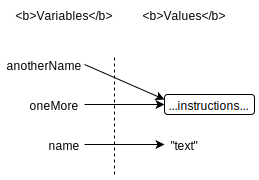
\includegraphics{../../files/callbacks-alias-function.svg}

As explained in \protect\hyperlink{s:basics}{the previous lesson}, when
JavaScript calls a function it assigns the arguments in the call to the
function's parameters. In order for this to be safe, we need to ensure
that there are no \protect\hyperlink{g:name-collision}{name collisions},
i.e., that if there is a variable called \texttt{something} and one of
the function's parameters is also called \texttt{something}, the
function will use the right one. The way every modern language
implements this is to use a \protect\hyperlink{g:call-stack}{call
stack}. Instead of putting all our variables in one big table, we have
one table for global variables and one extra table for each function
call. This means that if we assign 100 to \texttt{x}, call
\texttt{oneMore(2\ *\ x\ +\ 1)}, and look at memory in the middle of
that call, we will find this:

The Call Stack

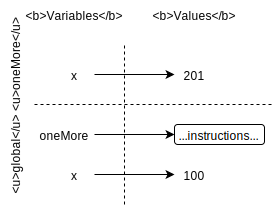
\includegraphics{../../files/callbacks-call-stack.svg}

\subsubsection{Functions of Functions}\label{s:callbacks-func}

The call stack allows us to write and call functions without worrying
about whether we're accidentally going to refer to the wrong variable.
And since functions are just another kind of data, we can pass one
function into another. For example, we can write a function called
\texttt{doTwice} that calls some other function two times:

\begin{verbatim}
const doTwice = (action) => {
  action()
  action()
}

const hello = () => {
  console.log('hello')
}

doTwice(hello)
\end{verbatim}

\begin{verbatim}
hello
hello
\end{verbatim}

Again, this is clearer when we look at the state of memory while
\texttt{doTwice} is running:

Functions of Functions

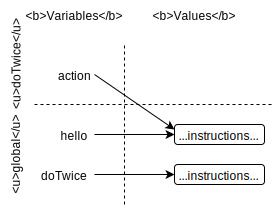
\includegraphics{../../files/callbacks-do-twice.svg}

This becomes more useful when the function or functions passed in have
parameters of their own. For example, the function \texttt{pipeline}
passes a value to one function, then takes that function's result and
passes it to a second, and returns the final result:

\begin{verbatim}
const pipeline = (initial, first, second) => {
  const temp = first(initial)
  return second(temp)
}
\end{verbatim}

Let's use this to combine a function that trims blanks off the starts
and ends of strings and another function that replaces spaces with dots:

\begin{verbatim}
const trim = (text) => { return text.trim() }
const dot = (text) => { return text.replace(/ /g, '.') }

const original = '  this example uses text  '

const trimThenDot = pipeline(original, trim, dot)
console.log(`trim then dot: |${trimThenDot}|`)
\end{verbatim}

\begin{verbatim}
trim then dot: |this.example.uses.text|
\end{verbatim}

During the call to \texttt{temp\ =\ first(initial)}, but before a value
has been returned to be assigned to \texttt{temp}, memory looks like
this:

Implementing a Pipeline

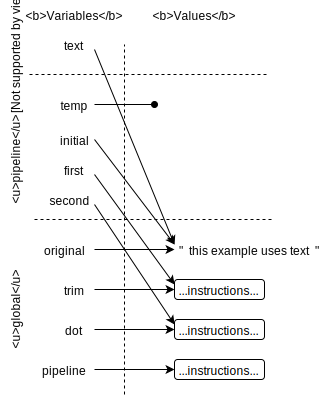
\includegraphics{../../files/callbacks-pipeline.svg}

Reversing the order of the functions changes the result:

\begin{verbatim}
const dotThenTrim = pipeline(original, dot, trim)
console.log(`dot then trim: |${dotThenTrim}|`)
\end{verbatim}

\begin{verbatim}
dot then trim: |..this.example.uses.text..|
\end{verbatim}

We can make a more general pipeline by passing an array of functions:

\begin{verbatim}
const pipeline = (initial, operations) => {
  let current = initial
  for (let op of operations) {
    current = op(current)
  }
  return current
}
\end{verbatim}

Let's add a function \texttt{double} to our suite of text manglers:

\begin{verbatim}
const double = (text) => { return text + text }
\end{verbatim}

and then try it out:

\begin{verbatim}
const original = ' some text '
const final = pipeline(original, [double, trim, dot])
console.log(`|${original}| -> |${final}|`)
\end{verbatim}

\begin{verbatim}
| some text | -> |some.text..some.text|
\end{verbatim}

\subsubsection{Anonymous Functions}\label{s:callbacks-anonymous}

Remember the function \texttt{oneMore}? We can pass it a value that we
have calculated on the fly:

\begin{verbatim}
oneMore = (x) => {
  return x + 1
}

console.log(oneMore(3 * 2))
\end{verbatim}

\begin{verbatim}
7
\end{verbatim}

Behind the scenes, JavaScript allocates a nameless temporary variable to
hold the value of \texttt{3\ *\ 2}, then passes a reference to that
temporary variable into \texttt{oneMore}. We can do the same thing with
functions, i.e., create one on the fly without giving it a name as we're
passing it into some other function. For example, suppose that instead
of pushing one value through a pipeline of functions, we want to call a
function once for each value in an array:

\begin{verbatim}
const transform = (values, operation) => {
  let result = []
  for (let v of values) {
    result.push(operation(v))
  }
  return result
}

const data = [10, 20, 30]
const result = transform(data, oneMore)
console.log(result)
\end{verbatim}

\begin{verbatim}
[ 11, 21, 31 ]
\end{verbatim}

Adding one to a number is such a simple thing to do that it's hardly
worth giving the function a name, so let's define it on the fly:

\begin{verbatim}
result = transform(data, (x) => {return x + 1})
console.log(result)
\end{verbatim}

\begin{verbatim}
[ 11, 21, 31 ]
\end{verbatim}

A function that is created this way is sometimes called an
\protect\hyperlink{g:anonymous-function}{anonymous function}, since its
creator doesn't give it a name. When JavaScript programmers use the term
``callback function'', they usually mean a function defined and used
like this.

\subsubsection{Functional Programming}\label{s:callbacks-functional}

\protect\hyperlink{g:functional-programming}{Functional programming} is
a style of programming that relies heavily on
\protect\hyperlink{g:higher-order-function}{higher-order functions} like
\texttt{pipeline} that take other functions as parameters. In addition,
functional programming expects that functions won't modify data in
place, but will instead create new data from old. For example, a true
believer in functional programming would be saddened by this:

\begin{verbatim}
const impure = (values) => {
  for (let i in values) {
    values[i] += 1
  }
}
\end{verbatim}

and would politely, even patiently, suggest that it be rewritten like
this:

\begin{verbatim}
const pure = (values) -> {
  result = []
  for (let v of values) {
    result.push(v + 1)
  }
  return result
}
\end{verbatim}

JavaScript arrays provide several methods to support functional
programming. For example, \texttt{Array.some} returns \texttt{true} if
\emph{any} element in an array passes a test, while \texttt{Array.every}
returns \texttt{true} if \emph{all} elements in an array pass a test.

Here's how they work:

\begin{verbatim}
const data = ['this', 'is', 'a', 'test']
console.log('some longer than 3:', data.some((x) => { return x.length > 3 }))
console.log('all longer than 3:', data.every((x) => { return x.length > 3 }))
\end{verbatim}

\begin{verbatim}
some longer than 3: true
all longer than 3: false
\end{verbatim}

\texttt{Array.filter} creates a new array containing only values that
pass a test:

\begin{verbatim}
const data = ['this', 'is', 'a', 'test']
console.log('those longer than 3:', data.filter((x) => { return x.length > 3 }))
\end{verbatim}

\begin{verbatim}
those longer than 3: [ 'this', 'test' ]
\end{verbatim}

\begin{itemize}
\tightlist
\item
  So do all of the elements with more than 3 characters start with a
  `t'?
\end{itemize}

\begin{verbatim}
const data = ['this', 'is', 'a', 'test']
const result = data
               .filter((x) => { return x.length > 3 })
               .every((x) => { return x[0] === 't' })
console.log(`all longer than 3 start with t: ${result}`)
\end{verbatim}

\begin{verbatim}
all longer than 3 start with t: true
\end{verbatim}

\texttt{Array.map} creates a new array by calling a function for each
element of an existing array:

\begin{verbatim}
const data = ['this', 'is', 'a', 'test']
console.log('shortened', data.map((x) => { return x.slice(0, 2) }))
\end{verbatim}

\begin{verbatim}
shortened [ 'th', 'is', 'a', 'te' ]
\end{verbatim}

And finally, \texttt{Array.reduce} reduces an array to a single value
using a combining function and a starting value. The combining function
must take two values, which are the current running total and the next
value from the array; if the array is empty, \texttt{Array.reduce}
returns the starting value.

\begin{verbatim}
const data = ['this', 'is', 'a', 'test']

const concatFirst = (accumulator, nextValue) => {
  return accumulator + nextValue[0]
}
let acronym = data.reduce(concatFirst, '')
console.log(`acronym of ${data} is ${acronym}`)

// In one step.
acronym = data.reduce((accum, next) => {
  return accum + next[0]
}, '')
console.log('all in one step:', acronym)
\end{verbatim}

\begin{verbatim}
acronym of this,is,a,test is tiat
all in one step: tiat
\end{verbatim}

The indentation of the ``in one step'' call may look a little odd, but
this is the style the JavaScript community has settled on.

\subsubsection{Closures}\label{s:callbacks-closures}

The last tool we need to introduce is an extremely useful side-effect of
the way memory is handled called a
\protect\hyperlink{g:closure}{closure}. The easiest way to explain it is
by example. We have already defined a function called \texttt{pipeline}
that chains any number of other functions together:

\begin{verbatim}
const pipeline = (initial, operations) => {
  let current = initial
  for (let op of operations) {
    current = op(current)
  }
  return current
}
\end{verbatim}

However, \texttt{pipeline} only works if each function in the array
\texttt{operations} has a single parameter. If we want to be able to add
1, add 2, and so on, we have to write separate functions, which is
annoying.

A better option is to write a function that creates the function we
want:

\begin{verbatim}
const adder = (increment) => {
  const f = (value) => {
    return value + increment
  }
  return f
}

const add_1 = adder(1)
const add_2 = adder(2)
console.log(`add_1(100) is ${add_1(100)} and add_2(100) is ${add_2(100)}`)
\end{verbatim}

\begin{verbatim}
add_1(100) is 101 and add_2(100) is 102
\end{verbatim}

The best way to understand what's going on is to draw a step-by-step
memory diagram. In step 1, we call \texttt{adder(1)}:

Creating an Adder (Step 1)

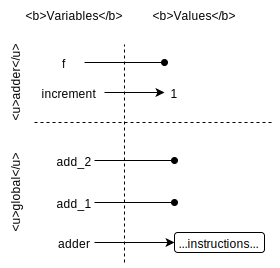
\includegraphics{../../files/callbacks-adder-1.svg}

\texttt{adder} creates a new function that includes a reference to that
1 we just passed in:

Creating an Adder (Step 2)

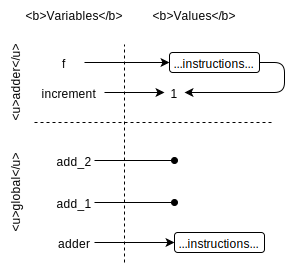
\includegraphics{../../files/callbacks-adder-2.svg}

In step 3, \texttt{adder} returns that function, which is assigned to
\texttt{add\_1}:

Creating an Adder (Step 3)

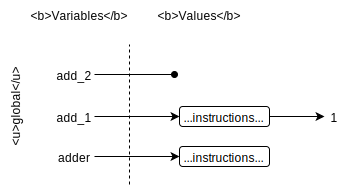
\includegraphics{../../files/callbacks-adder-3.svg}

Crucially, the function that \texttt{add\_1} refers to still has a
reference to the value 1, even though that value isn't referred to any
longer by anyone else.

In steps 4-6, we repeat these three steps to create another function
that has a reference to the value 2, and assign that function to
\texttt{add\_2}:

Creating an Adder (Steps 4-6)

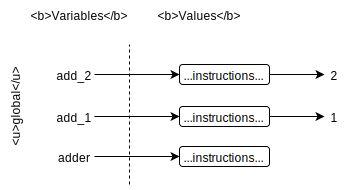
\includegraphics{../../files/callbacks-adder-4.svg}

When we now call \texttt{add\_1} or \texttt{add\_2}, they add the value
passed in and the value they've kept a reference to.

This trick of capturing a reference to a value inside something else is
called a \protect\hyperlink{g:closure}{closure}. It works because
JavaScript holds on to values as long as anything, anywhere, still
refers to them. Closures solve our pipeline problem by letting us define
little functions on the fly and give them extra data to work with:

\begin{verbatim}
const result = pipeline(100, [adder(1), adder(2)])
console.log(`adding 1 and 2 to 100 -> ${result}`)
\end{verbatim}

\begin{verbatim}
adding 1 and 2 to 100 -> 103
\end{verbatim}

Again, \texttt{adder(1)} and \texttt{adder(2)} do not add anything to
anything: they define new (unnamed) functions that add 1 and 2
respectively when called.

Programmers often go one step further and define little functions like
this inline:

\begin{verbatim}
const result = pipeline(100, [(x) => x + 1, (x) => x + 2])
console.log(`adding 1 and 2 to 100 -> ${result}`)
\end{verbatim}

\begin{verbatim}
adding 1 and 2 to 100 -> 103
\end{verbatim}

As this example shows, if the body of a function is a single expression,
it doesn't have to be enclosed in \texttt{\{...\}} and \texttt{return}
doesn't need to be used.

\subsubsection{Exercises}\label{s:callbacks-exercises}

\paragraph{\texorpdfstring{Side Effects With
\texttt{forEach}}{Side Effects With forEach}}\label{side-effects-with-foreach}

JavaScript arrays have a method called \texttt{forEach}, which calls a
callback function once for each element of the array. Unlike
\texttt{map}, \texttt{forEach} does \emph{not} save the values returned
by these calls or return an array of results. The full syntax is:

\begin{verbatim}
someArray.forEach((value, location, container) => {
  // 'value' is the value in 'someArray'
  // 'location' is the index of that value
  // 'container' is the containing array (in this case, 'someArray')
})
\end{verbatim}

If you only need the value, you can provide a callback that only takes
one parameter; if you only need the value and its location, you can
provide a callback that takes two.

Use this to write a function \texttt{doubleInPlace} that doubles all the
values in an array in place:

\begin{verbatim}
const vals = [1, 2, 3]
doubleInPlace(vals)
console.log(`vals after change: ${vals}`)
\end{verbatim}

\begin{verbatim}
vals after change: 2,4,6
\end{verbatim}

\paragraph{Annotating Data}\label{annotating-data}

Given an array of objects representing observations of wild animals:

\begin{verbatim}
data = [
  {'date': '1977-7-16', 'sex': 'M', 'species': 'NL'},
  {'date': '1977-7-16', 'sex': 'M', 'species': 'NL'},
  {'date': '1977-7-16', 'sex': 'F', 'species': 'DM'},
  {'date': '1977-7-16', 'sex': 'M', 'species': 'DM'},
  {'date': '1977-7-16', 'sex': 'M', 'species': 'DM'},
  {'date': '1977-7-16', 'sex': 'M', 'species': 'PF'},
  {'date': '1977-7-16', 'sex': 'F', 'species': 'PE'},
  {'date': '1977-7-16', 'sex': 'M', 'species': 'DM'}
]
\end{verbatim}

write a function that returns a new array of objects like this:

\begin{verbatim}
newData = [
  {'seq': 3, 'year': '1977', 'sex': 'F', 'species': 'DM'},
  {'seq': 7, 'year': '1977', 'sex': 'F', 'species': 'PE'}
]
\end{verbatim}

\emph{without} using any loops. The changes are:

\begin{itemize}
\tightlist
\item
  The \texttt{date} field is replaced with just the `year.
\item
  Only observations of female animals are retained.
\item
  The retained records are given sequence numbers to relate them back to
  the original data. (These sequence numbers are 1-based rather than
  0-based.)
\end{itemize}

You will probably want to use \texttt{Array.reduce} to generate the
sequence numbers.

\textbf{Key Points}

\begin{itemize}
\tightlist
\item
  JavaScript stores the instructions making up a function in memory like
  any other object.
\item
  Function objects can be assigned to variables, put in lists, passed as
  arguments to other functions, etc.
\item
  Functions can be defined in place without ever being given a name.
\item
  A callback function is one that is passed in to another function for
  it to execute at a particular moment.
\item
  Functional programming uses higher-order functions on immutable data.
\item
  \texttt{Array.some} is true if any element in an array passes a test,
  while \texttt{Array.every} is true if they all do.
\item
  \texttt{Array.filter} selects elements of an array that pass a test.
\item
  \texttt{Array.map} creates a new array by transforming values in an
  existing one.
\item
  \texttt{Array.reduce} reduces an array to a single value.
\item
  A closure is a set of variables captured during the definition of a
  function.
\end{itemize}

\hypertarget{s:oop}{\subsection{Objects and Classes}\label{s:oop}}

\textbf{Questions}

\begin{itemize}
\tightlist
\item
  How can I use classes to keep code and data together?
\item
  What are the benefits of doing this?
\item
  How can I create an object from a class?
\item
  How can I initialize that object?
\item
  How can I create new classes from old?
\item
  How does JavaScript decide what to do when two classes define the same
  thing?
\item
  When should I create new classes and when should I combine existing
  ones?
\item
  How can old code use new code?
\end{itemize}

Making new code use old code is easy: just load the libraries you want
and write calls to the functions you need. Making \emph{old} code use
\emph{new} code without rewriting it is trickier, but object-oriented
programming can help.

\subsubsection{Doing It By Hand}\label{s:oop-manual}

As we saw \protect\hyperlink{s:basics}{earlier}, an object in JavaScript
is a set of key-value pairs. Since functions are just another kind of
data, an object's values can be functions, so data can carry around
functions that work on it. For example, we can create an object to
represent a square:

\begin{verbatim}
const square = {
  name: 'square',
  size: 5,
  area: (it) => { return it.size * it.size },
  perimeter: (it) => { return 4 * it.size }
}
\end{verbatim}

and then pass the object itself into each of its own functions:

\begin{verbatim}
const a = square.area(square)
console.log(`area of square is ${a}`)
\end{verbatim}

\begin{verbatim}
area of square is 25
\end{verbatim}

This is a bit clumsy---we'll often forget to pass the object into its
functions---but it allows us to handle many different kinds of things in
the same way. For example, we can create another object to represent a
circle:

\begin{verbatim}
const circle = {
  name: 'circle',
  radius: 3,
  area: (it) => { return Math.PI * it.radius * it.radius },
  perimeter: (it) => { return 2 * Math.PI * it.radius }
}
\end{verbatim}

and then put all of these different objects in an array and operate on
them in the same way without knowing precisely what kind of object we're
dealing with:

\begin{verbatim}
const show_all = (shapes) => {
  for (let s of shapes) {
    const a = s.area(s)
    const p = s.perimeter(s)
    console.log(`${s.name}: area ${a} perimeter ${p}`)
  }
}

show_all([square, circle])
\end{verbatim}

\begin{verbatim}
square: area 25 perimeter 20
circle: area 28.274333882308138 perimeter 18.84955592153876
\end{verbatim}

As long as we only use the value \texttt{name} and the functions
\texttt{area} and \texttt{perimeter} we don't need to know what kind of
shape we have. This is called
\protect\hyperlink{g:polymorphism}{polymorphism}, and it allows us to
add new shapes without changing the code in our loop. In other words, it
allows old code (in this case, the function \texttt{show\_all}) to use
new code (the new object \texttt{rectangle}).

\begin{verbatim}
const rectangle = {
  name: 'rectangle',
  width: 2,
  height: 3,
  area: (it) => { return it.width * it.height },
  perimeter: (it) => { return 2 * (it.width + it.height) }
}

show_all([square, circle, rectangle])
\end{verbatim}

\begin{verbatim}
square: area 25 perimeter 20
circle: area 28.274333882308138 perimeter 18.84955592153876
rectangle: area 6 perimeter 10
\end{verbatim}

\subsubsection{Classes}\label{s:oop-classes}

Building every object by hand and calling \texttt{thing.function(thing)}
is clumsy. JavaScript solved these problems using
\protect\hyperlink{g:prototype}{prototypes}, which also turned out to be
\protect\hyperlink{s:legacy-prototypes}{clumsy}. Most object-oriented
languages use \protect\hyperlink{g:class}{classes} instead; these were
added to JavaScript in ES6, and we will use them instead of prototypes
throughout. Here's how we create a class that defines the properties of
a square, without actually creating any specific squares:

\begin{verbatim}
class Square {
  constructor (size) {
    this.name = 'square'
    this.size = size
  }
  area () { return this.size * this.size }
  perimeter () { return 4 * this.size }
}
\end{verbatim}

(Class names are written in CamelCase by convention.) We can then create
a specific square by using the class's name as if it were a function:

\begin{verbatim}
const sq = Square(3)
console.log(`sq name ${sq.name} and area ${sq.area()}`)
\end{verbatim}

\begin{verbatim}
sq name square and area 9
\end{verbatim}

\texttt{new\ ClassName(...)} creates a new blank object and inserts a
(hidden) reference to the class so that the object can find its
\protect\hyperlink{g:method}{methods}. \texttt{new} then calls the
specially-named method \texttt{constructor} to initialize the object's
state. Inside the constructor and other methods, the object being
operated on is referred to by the pronoun \texttt{this}.

Inside the class, methods are defined with classic syntax rather than
the \protect\hyperlink{g:fat-arrow}{fat arrows} we have been using. The
inconsistency is unfortunate but this way of defining methods is what
the current version of Node prefers; we will explore this topic further
in the \protect\hyperlink{s:vis}{discussion of visualization}.

Classes defined this way support polymorphism: if two or more classes
have some methods with the same names that take the same parameters and
return the same kinds of values, other code can use objects of those
classes interchangeably. For example, here's a class-based rewrite of
our shapes code:

\begin{verbatim}
class Circle {
  constructor (radius) {
    this.name = 'circle'
    this.radius = radius
  }
  area () { return Math.PI * this.radius * this.radius }
  perimeter () { return 2 * Math.PI * this.radius }
}

class Rectangle {
  constructor (width, height) {
    this.name = 'rectangle'
    this.width = width
    this.height = height
  }
  area () { return this.width * this.height }
  perimeter () { return 2 * (this.width + this.height) }
}

const everything = [
  new Square(3.5),
  new Circle(2.5),
  new Rectangle(1.5, 0.5)
]
for (let thing of everything) {
  const a = thing.area(thing)
  const p = thing.perimeter(thing)
  console.log(`${thing.name}: area ${a} perimeter ${p}`)
}
\end{verbatim}

\begin{verbatim}
square: area 12.25 perimeter 14
circle: area 19.634954084936208 perimeter 15.707963267948966
rectangle: area 0.75 perimeter 4
\end{verbatim}

\subsubsection{Inheritance}\label{s:oop-inheritance}

We can build new classes from old ones by adding or
\protect\hyperlink{g:override-method}{overriding} methods. To show this,
we'll start by defining a person:

\begin{verbatim}
class Person {
  constructor (name) {
    this.name = name
  }

  greeting (formal) {
    if (formal) {
      return `Hello, my name is ${this.name}`
    } else {
      return `Hi, I'm ${this.name}`
    }
  }

  farewell () {
    return `Goodbye`
  }
}
\end{verbatim}

We can now \protect\hyperlink{g:extend}{extend} \texttt{Person} to
create a new class \texttt{Scientist}, in which case we say that
\texttt{Scientist} \protect\hyperlink{g:inherit}{inherits} from
\texttt{Person}, or that \texttt{Person} is a
\protect\hyperlink{g:parent-class}{parent class} of \texttt{Scientist}
and \texttt{Scientist} is a \protect\hyperlink{g:child-class}{child
class} of \texttt{Person}.

\begin{verbatim}
class Scientist extends Person {
  constructor (name, area) {
    super(name)
    this.area = area
  }

  greeting (formal) {
    return `${super.greeting(formal)}. Let me tell you about ${this.area}...`
  }
}
\end{verbatim}

This tells us that a \texttt{Scientist} is a \texttt{Person} who:

\begin{itemize}
\tightlist
\item
  Has an area of specialization as well as a name.
\item
  Says hello in a slightly longer way
\item
  Says goodbye in the same way as a \texttt{Person} (since
  \texttt{Scientist} \emph{doesn't} define its own \texttt{farewell}
  method)
\end{itemize}

The word \texttt{super} is used in two ways here:

\begin{itemize}
\tightlist
\item
  In the constructor for \texttt{Scientist}, \texttt{super(...)} calls
  up to the constructor of the parent class \texttt{Person} so that it
  can do whatever initialization it does before \texttt{Scientist} does
  its own initialization. This saves us from duplicating steps.
\item
  Inside \texttt{greeting}, the expression
  \texttt{super.greeting(formal)} means ``call the parent class's
  \texttt{greeting} method for this object''. This allows methods
  defined in child classes to add to or modify the behavior of methods
  defined in parent classes, again without duplicating code.
\end{itemize}

Let's try it out:

\begin{verbatim}
const parent = new Person('Hakim')
console.log(`parent: ${parent.greeting(true)} - ${parent.farewell()}`)

const child = new Scientist('Bhadra', 'microbiology')
console.log(`child: ${child.greeting(false)} - ${child.farewell()}`)
\end{verbatim}

\begin{verbatim}
parent: Hello, my name is Hakim - Goodbye
child: Hi, I'm Bhadra. Let me tell you about microbiology... - Goodbye
\end{verbatim}

The diagram below shows what memory looks like after these classes have
been defined and the objects \texttt{parent} and \texttt{child} have
been created. It looks complex at first, but allows us to see how
JavaScript finds the right method when \texttt{child.farewell()} is
called:

\begin{itemize}
\tightlist
\item
  It looks in the object \texttt{child} to see if there's a function
  there with the right name.
\item
  There isn't, so it follows \texttt{child}'s link to its class
  \texttt{Scientist} to see if a function is there.
\item
  There isn't, so it follows the link from \texttt{Scientist} to the
  parent class \texttt{Person} and finds the function it's looking for.
\end{itemize}

Object-Oriented Inheritance

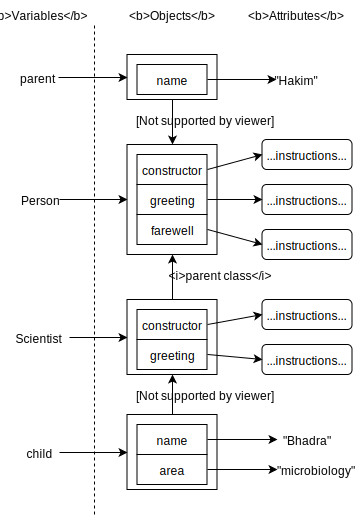
\includegraphics{../../files/oop-inheritance.svg}

\hypertarget{s:oop-protocols}{\subsubsection{Protocols}\label{s:oop-protocols}}

A common way to use object-oriented programming is to define a
\protect\hyperlink{g:protocol}{protocol}. The parent defines a method
that invokes other methods at specific times or in a specific order.
Users then derive classes from the parent that implement those methods
to do those specific things. In essence, a protocol says, ``You will all
follow this procedure, but you may follow it in different ways.''

For example, how does a generic bird behave throughout the year? The
class \texttt{Bird} specifies that it forages, mates, and nests, and
provides default methods for each:

\begin{verbatim}
class Bird {
  constructor (species) {
    this.species = species
  }

  daily (season) {
    return [
      this.foraging(season),
      this.mating(season),
      this.nesting(season)
    ]
  }

  foraging (season) {
    return `${this.species} looks for food`
  }

  mating (season) {
    let result = ''
    if (season === 'fall') {
      result = `${this.species} looks for a mate`
    }
    return result
  }

  nesting (season) {
    // do nothing
  }
}
\end{verbatim}

A specific kind of bird, such as a penguin, can then override these
methods to provide its own behaviors \emph{without} changing its daily
behavior:

\begin{verbatim}
class Penguin extends Bird {
  constructor () {
    super('penguin')
    this.hasEgg = false
  }

  mating (season) {
    if (season === 'fall') {
      this.hasEgg = Math.random() < 0.5
    }
    return super.mating(season)
  }

  nesting (season) {
    let result = ''
    if (this.hasEgg && ((season === 'winter') || (season === 'spring'))) {
      result = `${this.species} is nesting`
      if (season === 'spring') {
        this.hasEgg = false
      }
    }
    return result
  }
}
\end{verbatim}

\texttt{Penguin} has some extra state (the variable
\texttt{this.hasEgg}), and calls its parent's constructor before setting
this up. It doesn't override the default behavior for \texttt{foraging},
but it extends the default behavior for \texttt{mating} and completely
replaces the default behavior for \texttt{nesting}. Here are the results
of watching one penguin for four seasons:

\begin{verbatim}
const bird = new Penguin()
const seasons = ['summer', 'fall', 'winter', 'spring']
for (let season of seasons) {
  console.log(`in ${season}: ${bird.daily(season)}`)
}
\end{verbatim}

\begin{verbatim}
in summer: penguin looks for food,,
in fall: penguin looks for food,penguin looks for a mate,
in winter: penguin looks for food,,
in spring: penguin looks for food,,
\end{verbatim}

Here's another:

\begin{verbatim}
in summer: penguin looks for food,,
in fall: penguin looks for food,penguin looks for a mate,
in winter: penguin looks for food,,penguin is nesting
in spring: penguin looks for food,,penguin is nesting
\end{verbatim}

Different random numbers produce different behaviors, which makes
testing hard: we'll see how to address this
\protect\hyperlink{s:testing}{later} The main idea, though, is how old
code can use new code: the old code defines expectations as an interface
and a protocol, and the new code implements that interface and respects
that protocol. We will see this idea over and over again as we build
applications using standard libraries.

\subsubsection{Exercises}\label{s:oop-exercises}

\paragraph{Delays}\label{delays}

Define a class called \texttt{Delay} whose \texttt{call} method always
returns the value given in the \emph{previous} call:

\begin{verbatim}
const example = new Delay('a')
for (let value of ['b', 'c', 'd']) {
  console.log(value, '->', example.call(value))
}
\end{verbatim}

\begin{verbatim}
b -> a
c -> b
d -> c
\end{verbatim}

A class like \texttt{Delay} is sometimes called
\protect\hyperlink{g:stateful}{stateful}, since it remembers its state
from call to call.

\paragraph{Filtering}\label{filtering}

Define a class called \texttt{Filter} whose \texttt{call} method returns
\texttt{null} if its input matches one of the values given to its
constructor, or the input as output otherwise:

\begin{verbatim}
const example = new Filter('a', 'e', 'i', 'o', 'u')
for (let value of ['a', 'b', 'c', 'd', 'e']) {
  console.log(value, '->', example.call(value))
}
\end{verbatim}

\begin{verbatim}
a -> null
b -> b
c -> c
d -> d
e -> null
\end{verbatim}

A class like \texttt{Filter} is sometimes called
\protect\hyperlink{g:stateless}{stateless}, since it does not remember
its state from call to call.

\paragraph{Pipelines}\label{pipelines}

Define a class called \texttt{Pipeline} whose constructor takes one or
more objects with a single-parameter \texttt{call} method, and whose own
\texttt{call} method passes a value through each of them in turn. If any
of the components' \texttt{call} methods returns \texttt{null},
\texttt{Pipeline} stops immediately and returns \texttt{null}.

\begin{verbatim}
const example = new Pipeline(new Filter('a', 'e', 'i', 'o', 'u'), new Delay('a'))
for (let value of ['a' ,'b', 'c', 'd', 'e']) {
  console.log(value, '->', example.call(value))
}
\end{verbatim}

\begin{verbatim}
a -> null
b -> a
c -> b
d -> c
e -> null
\end{verbatim}

\paragraph{Active Expressions}\label{active-expressions}

Consider this class:

\begin{verbatim}
class Active {
  constructor (name, transform) {
    this.name = name
    this.transform = transform
    this.subscribers = []
  }

  subscribe (someone) {
    this.subscribers.push(someone)
  }

  update (input) {
    console.log(this.name, 'got', input)
    const output = this.transform(input)
    for (let s of this.subscribers) {
      s.update(output)
    }
  }
}
\end{verbatim}

and this program that uses it:

\begin{verbatim}
const start = new Active('start', (x) => Math.min(x, 10))
const left = new Active('left', (x) => 2 * x)
const right = new Active('right', (x) => x + 1)
const final = new Active('final', (x) => x)
start.subscribe(left)
start.subscribe(right)
left.subscribe(final)
right.subscribe(final)

start.update(123)
\end{verbatim}

\begin{enumerate}
\tightlist
\item
  Trace what happens when the last line of the program is called.
\item
  Modify \texttt{Active} so that it calls \texttt{transform} \emph{if}
  that function was provided, or a method \texttt{Active.transform} if a
  transformation function wasn't provided.
\item
  Create a new class \texttt{Delay} whose \texttt{transform} method
  always returns the previous value. (Its constructor will need to take
  an initial value as a parameter.)
\end{enumerate}

This pattern is called
\protect\hyperlink{g:observer-observable}{observer/observable}.

\textbf{Key Points}

\begin{itemize}
\tightlist
\item
  Create classes to define combinations of data and behavior.
\item
  Use the class's constructor to initialize objects.
\item
  \texttt{this} refers to the current object.
\item
  Use polymorphism to express common behavior patterns.
\item
  Extend existing classes to create new ones-sometimes.
\item
  Override methods to change or extend their behavior.
\item
  Creating extensible systems by defining interfaces and protocols.
\end{itemize}

\hypertarget{s:htmlcss}{\subsection{HTML and CSS}\label{s:htmlcss}}

\textbf{Questions}

\begin{itemize}
\tightlist
\item
  Where did HTML come from?
\item
  What kinds of things can HTML pages contain?
\item
  How do I create headings? Lists? Tables? Links?
\item
  How do I include images?
\item
  How can I change the appearance of elements on a page?
\item
  How can I reference specific elements on a page?
\end{itemize}

HTML is the standard way to represent documents for presentation in web
browsers, and CSS is the standard way to describe how it should look.
Both are more complicated than they should have been, but in order to
create web applications, we need to understand a little of both.

\subsubsection{Formatting}\label{s:htmlcss-formatting}

An HTML \protect\hyperlink{g:document}{document} contains
\protect\hyperlink{g:element}{elements} and text (and possibly other
things that we will ignore for now). Elements are shown using
\protect\hyperlink{g:tag}{tags}: an opening tag
\texttt{\textless{}tagname\textgreater{}} shows where the element
begins, and a corresponding closing tag
\texttt{\textless{}/tagname\textgreater{}} (with a leading slash) shows
where it ends. If there's nothing between the two, we can write
\texttt{\textless{}tagname/\textgreater{}} (with a trailing slash).

A document's elements must form a \protect\hyperlink{g:tree}{tree},
i.e., they must be strictly nested. This means that if Y starts inside
X, Y must end before X ends, so
\texttt{\textless{}X\textgreater{}...\textless{}Y\textgreater{}...\textless{}/Y\textgreater{}\textless{}/X\textgreater{}}
is legal, but
\texttt{\textless{}X\textgreater{}...\textless{}Y\textgreater{}...\textless{}/X\textgreater{}\textless{}/Y\textgreater{}}
is not. Finally, every document should have a single
\protect\hyperlink{g:root-element}{root element} that encloses
everything else, although browsers aren't strict about enforcing this.
In fact, most browsers are pretty relaxed about enforcing any kind of
rules at all, since most people don't obey them anyway.

\subsubsection{Text}\label{s:htmlcss-text}

The text in an HTML page is normal printable text. However, since
\texttt{\textless{}} and \texttt{\textgreater{}} are used to show where
tags start and end, we must use
\protect\hyperlink{g:escape-sequence}{escape sequences} to represent
them, just as we use \texttt{\textbackslash{}"} to represented a literal
double-quote character inside a double-quoted string in JavaScript. In
HTML, escape sequences are written \texttt{\&name;}, i.e., an ampersand,
the name of the character, and a semi-colon. A few common escape
sequences include:

\begin{longtable}[]{@{}lll@{}}
\toprule
Name & Escape Sequence & Character\tabularnewline
\midrule
\endhead
Less than & \texttt{\&lt;} & \textless{}\tabularnewline
Greater than & \texttt{\&gt;} & \textgreater{}\tabularnewline
Ampersand & \texttt{\&amp;} & \&\tabularnewline
Copyright & \texttt{\&copy;} & ©\tabularnewline
Plus/minus & \texttt{\&plusmn;} & ±\tabularnewline
Micro & \texttt{\&micro;} & µ\tabularnewline
\bottomrule
\end{longtable}

The first two are self-explanatory, and \texttt{\&amp;} is needed so
that we can write a literal ampersand (just as
\texttt{\textbackslash{}\textbackslash{}} is needed in JavaScript
strings so that we can write a literal backslash). \texttt{\&copy;},
\texttt{\&plusmn;}, and \texttt{\&micro;} are usually not needed any
longer, since most editors will allow us to put non-ASCII characters
directly into documents these days, but occasionally we will run into
older or stricter systems.

\subsubsection{Pages}\label{s:htmlcss-pages}

An HTML page should have:

\begin{itemize}
\tightlist
\item
  a single \texttt{html} element that encloses everything else
\item
  a single \texttt{head} element that contains information about the
  page
\item
  a single \texttt{body} element that contains the content to be
  displayed
\end{itemize}

It doesn't matter whether or how we indent the tags showing these
elements and the content they contain, but laying them out on separate
lines and indenting to show nesting helps human readers. Well-written
pages also use comments, just like code: these start with
\texttt{\textless{}!-\/-} and end with \texttt{-\/-\textgreater{}}.
Unfortunately, comments cannot be nested, i.e., if you comment out a
section of a page that already contains a comment, the results are
unpredictable.

Here's an empty HTML page with the structure described above:

\begin{verbatim}
<html>
  <head>
    <!-- description of page goes here -->
  </head>
  <body>
    <!-- content of page goes here -->
  </body>
</html>
\end{verbatim}

Nothing shows up if we open this in a browser, so let's add a little
content:

\begin{verbatim}
<html>
  <head>
    <title>This text is displayed in the browser bar</title>
  </head>
  <body>
    <h1>Displayed Content Starts Here</h1>
    <p>
      This course introduces core features of <em>JavaScript</em>
      and shows where and how to use them.
    </p>
    <!-- The word "JavaScript" is in italics (emphasis) in the preceding paragraph. -->
  </body>
</html>
\end{verbatim}

\begin{itemize}
\tightlist
\item
  The \texttt{title} element inside \texttt{head} gives the page a
  title. This is displayed in the browser bar when the page is open, but
  is \emph{not} displayed as part of the page itself.
\item
  The \texttt{h1} element is a level-1 heading; we can use \texttt{h2},
  \texttt{h3}, and so on to create sub-headings.
\item
  The \texttt{p} element is a paragraph.
\item
  Inside a heading or a paragraph, we can use \texttt{em} to
  \emph{emphasize} text. We can also use \texttt{strong} to make text
  \textbf{stronger}. Tags like these are better than tags like
  \texttt{i} (for italics) or \texttt{b} (for bold) because they signal
  intention rather than forcing a particular layout. Someone who is
  visually impaired, or someone using a small-screen device, may want
  emphasis of various kinds displayed in different ways.
\end{itemize}

\subsubsection{Attributes}\label{s:htmlcss-attributes}

Elements can be customized by giving them
\protect\hyperlink{g:attribute}{attributes}, which are written as
\texttt{name="value"} pairs inside the element's opening tag. For
example:

\begin{verbatim}
<h1 align="center">A Centered Heading</h1>
\end{verbatim}

centers the \texttt{h1} heading on the page, while:

\begin{verbatim}
<p class="disclaimer">This planet provided as-is.</p>
\end{verbatim}

marks this paragraph as a disclaimer. That doesn't mean anything special
to HTML, but as we'll see later, we can define styles based on the
\texttt{class} attributes of elements.

An attribute's name may appear at most once in any element, just like a
key can only appear once in any JavaScript object, so
\texttt{\textless{}p\ align="left"\ align="right"\textgreater{}...\textless{}/p\textgreater{}}
is illegal. If we want to give an attribute multiple values---for
example, if we want an element to have several classes---we put all the
values in one string. Unfortunately, as the example below shows, HTML is
inconsistent about whether values should be separated by spaces or
semi-colons:

\begin{verbatim}
<p class="disclaimer optional" style="color: blue; font-size: 200%;">
\end{verbatim}

However they are separated, values are supposed to be quoted, but in
practice we can often get away with \texttt{name=value}. And for Boolean
attributes whose values are just true or false, we can even sometimes
just get away with \texttt{name} on its own.

\subsubsection{Lists}\label{s:htmlcss-lists}

Headings and paragraphs are all very well, but data scientists need
more. To create an unordered (bulleted) list, we use a \texttt{ul}
element, and wrap each item inside the list in \texttt{li}. To create an
ordered (numbered) list, we use \texttt{ol} instead of \texttt{ul}, but
still use \texttt{li} for the list items.

\begin{verbatim}
<ul>
  <li>first</li>
  <li>second</li>
  <li>third</li>
</ul>
\end{verbatim}

\begin{itemize}
\tightlist
\item
  first
\item
  second
\item
  third
\end{itemize}

\begin{verbatim}
<ol>
  <li>first</li>
  <li>second</li>
  <li>third</li>
</ol>
\end{verbatim}

\begin{enumerate}
\tightlist
\item
  first
\item
  second
\item
  third
\end{enumerate}

Lists can be nested by putting the inner list's \texttt{ul} or
\texttt{ol} inside one of the outer list's \texttt{li} elements:

\begin{verbatim}
<ol>
  <li>Major A
    <ol>
      <li>minor p</li>
      <li>minor q</li>
    </ol>
  </li>
  <li>Major B
    <ol>
      <li>minor r</li>
      <li>minor s</li>
    </ol>
  </li>
</ol>
\end{verbatim}

\begin{enumerate}
\tightlist
\item
  Major A

  \begin{enumerate}
  \tightlist
  \item
    minor p
  \item
    minor q
  \end{enumerate}
\item
  Major B

  \begin{enumerate}
  \tightlist
  \item
    minor r
  \item
    minor s
  \end{enumerate}
\end{enumerate}

\subsubsection{Tables}\label{s:htmlcss-tables}

Lists are a great way to get started, but if we \emph{really} want to
impress people with our data science skills, we need tables.
Unsurprisingly, we use the \texttt{table} element to create these. Each
row is a \texttt{tr} (for ``table row''), and within rows, column items
are shown with \texttt{td} (for ``table data'') or \texttt{th} (for
``table heading'').

\begin{verbatim}
<table>
  <tr> <th>Alkali</th>   <th>Noble Gas</th> </tr>
  <tr> <td>Hydrogen</td> <td>Helium</td>    </tr>
  <tr> <td>Lithium</td>  <td>Neon</td>      </tr>
  <tr> <td>Sodium</td>   <td>Argon</td>     </tr>
</table>
\end{verbatim}

\begin{longtable}[]{@{}ll@{}}
\toprule
Alkali & Noble Gas\tabularnewline
\midrule
\endhead
Hydrogen & Helium\tabularnewline
Lithium & Neon\tabularnewline
Sodium & Argon\tabularnewline
\bottomrule
\end{longtable}

Do \emph{not} use tables to create multi-column layouts: there's a
better way.

\subsubsection{Links}\label{s:htmlcss-links}

Links to other pages are what makes HTML hypertext. Confusingly, the
element used to show a link is called \texttt{a}. The text inside the
element is displayed and (usually) highlighted for clicking. Its
\texttt{href} attribute specifies what the link is pointing at; both
local filenames and URLs are supported. Oh, and we can use
\texttt{\textless{}br/\textgreater{}} to force a line break in text
(with a trailing slash inside the tag, since the \texttt{br} element
doesn't contain any content):

\begin{verbatim}
<a href="https://nodejs.org/">Node.js</a>
<br/>
<a href="https://facebook.github.io/react/">React</a>
<br/>
<a href="../index.html">home page (relative path)</a>
\end{verbatim}

\href{https://nodejs.org/}{Node.js}\\
\href{https://facebook.github.io/react/}{React}\\
\href{../index.html}{home page (relative path)}

\subsubsection{Images}\label{s:htmlcss-images}

Images can be stored inside HTML pages in two ways: by using SVG (which
we will discuss \protect\hyperlink{s:vis}{later} or by encoding the
image as text and including that text in the body of the page, which is
clever, but makes the source of the pages very hard to read.

It is far more common to store each image in a separate file and refer
to that file using an \texttt{img} element (which also allows us to use
the image in many places without copying it). The \texttt{src} attribute
of the \texttt{img} tag specifies where to find the file; as with the
\texttt{href} attribute of an \texttt{a} element, this can be either a
URL or a local path. Every \texttt{img} should also include a
\texttt{title} attribute (whose purpose is self-explanatory) and an
\texttt{alt} attribute with some descriptive text to aid accessibility
and search engines.

\begin{verbatim}
<img src="./html5.png" title="HTML5 Logo" alt="Displays the HTML5 logo using a local path" />
<img src="https://github.com/software-tools-in-javascript/js-vs-rc/blob/master/src/htmlcss/html5.png"
     title="HTML5 Logo" alt="Display the HTML5 logo using a URL" />
\end{verbatim}

Two things are worth noting here:

\begin{enumerate}
\tightlist
\item
  Since \texttt{img} elements don't contain any text, they are often
  written with the trailing-slash notation. However, they are also often
  written improperly as \texttt{\textless{}img\ src="..."\textgreater{}}
  without any slashes at all. Browsers will understand this, but some
  software packages will complain.
\item
  If an image file is referred to using a path rather than a URL, that
  path can be either \protect\hyperlink{g:relative-path}{relative} or
  \protect\hyperlink{g:absolute-path}{absolute}. If it's a relative
  path, it's interpreted starting from where the web page is located; if
  it's an absolute path, it's interpreted relative to wherever the web
  browser thinks the \protect\hyperlink{g:root-directory}{root
  directory} of the filesystem is. As we will see
  \protect\hyperlink{s:server}{later}, this can change from one
  installation to the next, so you should always try to use relative
  paths, except where you can't. It's all very confusing\ldots{}
\end{enumerate}

\subsubsection{Cascading Style Sheets}\label{s:htmlcss-css}

When HTML first appeared, people styled elements by setting their
attributes:

\begin{verbatim}
<html>
  <body>
    <h1 align="center">Heading is Centered</h1>
    <p>
      <b>Text</b> can be highlighted
      or <font color="coral">colorized</font>.
    </p>
  </body>
</html>
\end{verbatim}

Many still do, but a better way is to use
\protect\hyperlink{g:css}{Cascading Style Sheets} (CSS). These allow us
to define a style once and use it many times, which makes it much easier
to maintain consistency. (I was going to say ``\ldots{}and keep pages
readable'', but given how complex CSS can be, that's not a claim I feel
I can make.) Here's a page that uses CSS instead of direct styling:

\begin{verbatim}
<html>
  <head>
    <link rel="stylesheet" href="simple-style.css" />
  </head>
  <body>
    <h1 class="title">Heading is Centered</h1>
    <p>
      <span class="keyword">Text</span> can be highlighted
      or <span class="highlight">colorized</span>.
    </p>
  </body>
</html>
\end{verbatim}

The \texttt{head} contains a link to a CSS file stored in the same
directory as the page itself; we could use a URL here instead of a
relative path, but the \texttt{link} element \emph{must} have the
\texttt{rel="stylesheet"} attribute. Inside the page, we then set the
\texttt{class} attribute of each element we want to style.

The file \texttt{simple-style.css} looks like this:

\begin{verbatim}
h1.title {
  text-align: center;
}
span.keyword {
  font-weight: bold;
}
.highlight {
  color: coral;
}
\end{verbatim}

Each entry has the form \texttt{tag.class} followed by a group of
properties inside curly braces, and each property is a key-value pair.
We can omit the class and just write (for example):

\begin{verbatim}
p {
  font-style: italic;
}
\end{verbatim}

in which case the style applies to everything with that tag. If we do
this, we can override general rules with specific ones: the style for a
disclaimer paragraph is defined by \texttt{p} with overrides defined by
\texttt{p.disclaimer}. We can also omit the tag and simply use
\texttt{.class}, in which case every element with that class has that
style.

As suggested by the earlier discussion of separators, elements may have
multiple values for class, as in
\texttt{\textless{}span\ class="keyword\ highlight"\textgreater{}...\textless{}/span\textgreater{}}.
(The \texttt{span} element simply marks a region of text, but has no
effect unless it's styled.)

These two features are one (but unfortunately not the only) common
source of confusion with CSS: If one may override general rules with
specific ones but also provide multiple values for class, how do we keep
track of which rules will apply to an element with multiple classes? A
detailed discussion of the order of precedence for CSS rules is outside
the scope of this tutorial. We recommend that those likely to work often
with stylesheets read (and consider bookmarking)
\href{https://www.w3schools.com/css/css_specificity.asp}{this W3Schools
page}.

One other thing CSS can do is match specific elements. We can label
particular elements uniquely within a page using the \texttt{id}
attribute, then refer to those elements using \texttt{\#name} as a
\protect\hyperlink{g:selector}{selector}. For example, if we create a
page that gives two spans unique IDs:

\begin{verbatim}
<html>
  <head>
    <link rel="stylesheet" href="selector-style.css" />
  </head>
  <body>
    <p>
      First <span id="major">keyword</span>.
    </p>
    <p>
      Full <span id="minor">explanation</span>.
    </p>
  </body>
</html>
\end{verbatim}

then we can style those spans like this:

\begin{verbatim}
#major {
  text-decoration: underline red;
}
#minor {
  text-decoration: overline blue;
}
\end{verbatim}

\begin{quote}
\textbf{Internal Links}

We can also link directly to an element within a page using
\texttt{\#name} inside the \texttt{href} attribute of a link. For
example,
\texttt{\textless{}a\ href="selectors.html\#major"\textgreater{}some\ text\textless{}/a\textgreater{}}
refers to the \texttt{\#major} element in \texttt{selectors.html}, while
\texttt{\textless{}a\ href="selectors.html\#minor"\textgreater{}some\ text\textless{}/a\textgreater{}}
refers to the \texttt{\#minor} element. This is particularly useful
\emph{within} pages:
\texttt{\textless{}a\ href="\#major"\textgreater{}jump\textless{}/a\textgreater{}}
takes us straight to the \texttt{\#major} element within this page.
Internal links like this are often used for cross-referencing and to
create a table of contents.
\end{quote}

\subsubsection{Bootstrap}\label{s:htmlcss-bootstrap}

CSS can become very complicated very quickly, so most people use a
framework to take care of the details. One of the most popular is
\href{https://getbootstrap.com/}{Bootstrap} (which is what we're using
to style this website). Here's the entire source of a page that uses
Bootstrap to create a two-column layout with a banner at the top:

\begin{verbatim}
<html>
  <head>
    <link rel="stylesheet" href="https://stackpath.bootstrapcdn.com/bootstrap/4.1.3/css/bootstrap.min.css">
    <style>
      div {
        border: solid 1px;
      }
    </style>
  </head>
  <body>

    <div class="jumbotron text-center">
      <h1>Page Title</h1>
      <p>Resize this page to see how the layout adjusts dynamically.</p>
    </div>

    <div class="container">
      <div class="row">
        <div class="col-sm-4">
          <h2>First column is 4 wide</h2>
          <p>Text here goes</p>
          <p>in the column</p>
        </div>
        <div class="col-sm-8">
          <h2>Second column is 8 wide</h2>
          <p>Text over here goes</p>
          <p>in the other column</p>
        </div>
      </div>
    </div>

  </body>
</html>
\end{verbatim}

The page opens by loading Bootstrap from the web; we can also download
\texttt{bootstrap.min.css} and refer to it with a local path. (The
\texttt{.min} in the file's name signals that the file has been
\protect\hyperlink{g:minimization}{minimized} so that it will load more
quickly.)

The page then uses a \texttt{style} element to create an
\protect\hyperlink{g:internal-style-sheet}{internal style sheet} to put
a solid one-pixel border around every \texttt{div} so that we can see
the regions of the page more clearly. Defining styles in the page header
is generally a bad idea, but it's a good way to test things quickly. Oh,
and a \texttt{div} just marks a region of a page without doing anything
to it, just as a \texttt{span} marks a region of text without changing
its appearance unless we apply a style.

The first \texttt{div} creates a header box (called a ``jumbotron'') and
centers its text. The second \texttt{div} is a container, which creates
a bit of margin on the left and right sides of our content. Inside that
container is a row with two columns, one 4/12 as wide as the row and the
other 8/12 as wide. (Bootstrap uses a 12-column system because 12 has
lots of divisors.)

Bootstrap is \protect\hyperlink{g:responsive-design}{responsive}:
elements change size as the page grows narrower, and are then stacked
when the screen becomes too small to display them side by side.

We've left out many other aspects of HTML and CSS as well, such as
figure captions, multi-column table cells, and why it's so hard to
center text vertically within a \texttt{div}. One thing we will return
to \protect\hyperlink{s:interactive}{later} is how to include
interactive elements like buttons and forms in a page. Handling those is
part of why JavaScript was invented in the first place, but we need more
experience before tackling them.

\subsubsection{Exercises}\label{s:htmlcss-exercises}

\paragraph{Cutting Corners}\label{cutting-corners}

What does your browser display if you forget to close a paragraph or
list item tag like this:

\begin{verbatim}
<p>This paragraph starts but doesn't officially end.

<p>Another paragraph starts here but also doesn't end.

<ul>
  <li>First item in the list isn't closed.
  <li>Neither is the second.
</ul>
\end{verbatim}

\begin{enumerate}
\tightlist
\item
  What happens if you don't close a \texttt{ul} or \texttt{ol} list?
\item
  Is that behavior consistent with what happens when you omit
  \texttt{\textless{}/p\textgreater{}} or
  \texttt{\textless{}/li\textgreater{}}?
\end{enumerate}

\paragraph{Mix and Match}\label{mix-and-match}

\begin{enumerate}
\tightlist
\item
  Create a page that contains a 2x2 table, each cell of which has a
  three-item bullet-point list. How can you reduce the indentation of
  the list items within their cells using CSS?
\item
  Open your page in a different browser (e.g., Firefox or Edge). Do they
  display your indented lists consistently?
\item
  Why do programs behave inconsistently? Why do programmers do this to
  us? Why? Why why why why why?
\end{enumerate}

\paragraph{Naming}\label{naming}

What does the \texttt{sm} in Bootstrap's \texttt{col-sm-4} and
\texttt{col-sm-8} stand for? What other options could you use instead?
Why do web developers still use FORTRAN-style names in the 21st Century?

\paragraph{Color}\label{color}

HTML and CSS define names for a small number of colors. All other colors
must be specified using \protect\hyperlink{g:rgb}{RGB} values. Write a
small JavaScript program that creates an HTML page that displays the
word \texttt{color} in 100 different randomly-generated colors. Compare
this to the color scheme used in your departmental website. Which one
hurts your eyes less?

\paragraph{Units}\label{units}

What different units can you use to specify text size in CSS? What do
they mean? What does \emph{anything} mean, when you get right down to
it?

\textbf{Key Points}

\begin{itemize}
\tightlist
\item
  HTML is the latest in a long line of markup languages.
\item
  HTML documents contain elements (represented by tags in angle
  brackets) and text.
\item
  Elements must be strictly nested.
\item
  Elements can contain attributes.
\item
  Use escape sequences beginning with ampersand to represent special
  characters.
\item
  Every page should have one \texttt{html} element containing a
  \texttt{head} and a \texttt{body}.
\item
  Use \texttt{\textless{}!-\/-...-\/-\textgreater{}} to include comments
  in HTML.
\item
  Use \texttt{ul} and \texttt{ol} for unordered and ordered lists, and
  \texttt{li} for list elements.
\item
  Use \texttt{table} for tables, \texttt{tr} for rows, \texttt{th} for
  headings, and \texttt{td} for regular data.
\item
  Use
  \texttt{\textless{}a\ href="..."\textgreater{}...\textless{}/a\textgreater{}}
  to create links.
\item
  Use
  \texttt{\textless{}img\ src="..."\ title="..."\ alt="..."\ /\textgreater{}}
  to include images.
\item
  Use CSS to define appearance of elements.
\item
  Use \texttt{class} and \texttt{id} to identify elements.
\item
  Use selectors to specify the elements that CSS applies to.
\end{itemize}

\hypertarget{s:pages}{\subsection{Manipulating Pages}\label{s:pages}}

\textbf{Questions}

\begin{itemize}
\tightlist
\item
  How can I find things in pages?
\item
  How can I change things in pages?
\item
  How can I interact with JavaScript in the browser?
\end{itemize}

We have presented a lot of tools, but as yet no applications. As a
reward for your patience, we will therefore work through several
examples that show how to do useful things to web pages. These examples
introduce some new concepts, the most important of which is the way in
which HTML pages are represented in, and manipulated by, JavaScript.

One thing these examples \emph{don't} show is how to build interactive
web pages. JavaScript was invented primarily to support buttons, forms,
and the like, but we will need to do a bit more background work before
exploring them. Still, we can do a surprising number of useful things
simply by playing with the content of pages.

\subsubsection{Counting Paragraphs}\label{s:pages-counting}

Let's begin by counting the number of paragraphs in a page:

\begin{verbatim}
<html>
  <head>
    <meta charset="utf-8"/>
  </head>
  <body>
    <h1>Title</h1>
    <div class="fill"></div>
    <h2 id="one">First <em>emphasized</em></h2>
    <p>stuff</p>
    <h2 id="two">Second <code>with code</code></h2>
    <h3>stuff</h3>
    <h2 id="three">Third</h2>
    <p>stuff</p>

    <script>
      const counter = () => {
        const paragraphs = document.querySelectorAll('p')
        return paragraphs.length
      }
      console.log(`number of paragraphs: ${counter()}`)
    </script>
  </body>
</html>
\end{verbatim}

This page has three main parts:

\begin{enumerate}
\item
  The \texttt{head} contains a \texttt{meta} tag that specifies the
  page's \protect\hyperlink{g:character-encoding}{character encoding},
  i.e., the scheme used to represent characters not found on a standard
  American keyboard in the 1970s. Character sets and character encodings
  are out of scope for this lesson; see
  \href{https://www.joelonsoftware.com/2003/10/08/the-absolute-minimum-every-software-developer-absolutely-positively-must-know-about-unicode-and-character-sets-no-excuses/}{this
  essay} for an unfortunately timeless discussion.
\item
  The top half of the \texttt{body} has some headings and paragraphs for
  the JavaScript to play with. It also contains a \texttt{div} marked
  with \texttt{class="fill"} that our script will eventually fill in
  with a count.
\item
  The script itself is contained in a \texttt{script} tag at the bottom
  of the page; we will explore it in depth below.
\end{enumerate}

\begin{quote}
\textbf{When Scripts Run}

We have put the script at the bottom of the page because we want to be
sure that the page's contents actually exist in memory before trying to
process them. If we put the \texttt{script} tag and its contents at the
top of the page, the browser might run our JavaScript \emph{after} the
page has been read but \emph{before} its elements and text have been
parsed and stored in memory. \protect\hyperlink{g:race-condition}{Race
conditions} like this bedevil web programming; we will see more robust
ways to deal with them later.
\end{quote}

Inside the \texttt{script} tag, we define a function called
\texttt{counter} that takes no arguments, then use \texttt{console.log}
to display the result of calling it. The only thing inside the function
that we haven't encountered before is the call
\texttt{document.querySelectorAll(\textquotesingle{}p\textquotesingle{})}.
As you might guess from its name, \texttt{document} is an object that
gives us a handle on the page the script is in; it is created and
provided automatically by the browser. Its \texttt{querySelectorAll}
method finds all elements in the page that match the selector we
provide. In this case, we're looking for all paragraphs, so we simply
search for \texttt{\textquotesingle{}p\textquotesingle{}}.

To see the JavaScript in action, run a browser, open its developer tools
so that you can see the JavaScript console, and then load the page. The
page's elements will be displayed as usual, and the console will show:

\begin{verbatim}
number of paragraphs: 2
\end{verbatim}

\begin{quote}
\textbf{Developer Tools}

If you are using the Firefox browser, you can open the developer tools
pane by going to the main menu and selecting
\texttt{Tools...\ Web\ Developer...\ Toggle\ Tools}. A tabbed display
will open in the bottom of your page; choose \texttt{Console} to view
the output of your JavaScript, or to write a little bit to run
immediately.
\end{quote}

Showing results in the console is good enough for development work, but
we would like to see the result in the page itself. To do this, we can
replace the call to \texttt{console.log} with the two lines shown below:

\begin{verbatim}
const counter = () => {
  const paragraphs = document.querySelectorAll('p')
  return paragraphs.length
}
const fill = document.getElementById('fill')
fill.innerHTML = `number of paragraphs: ${counter()}`
\end{verbatim}

Where \texttt{document.querySelectorAll} returns all nodes that match a
selector, \texttt{document.getElementById} returns a single element that
has the specified ID (which is set inside the element's opening tag with
\texttt{id="some\_name"}). The variable \texttt{fill} is therefore
assigned a reference to our \texttt{div}. We can then change the text
inside that element by assigning to its \texttt{innerHTML} property.
When we do this, JavaScript parses the string we provided as if it were
HTML and creates whatever nodes it needs to represent the result. In
this case, the content is just text, so JavaScript will create a single
text node, store \texttt{"number\ of\ paragraphs:\ 2"} as its content,
and add it to the in-memory structure that represents the page.

\ldots{}at which point some magic happens behind the scenes. The browser
stores the elements and text of the current page in a data structure
called the Document Object Model, or more commonly, the
\protect\hyperlink{g:dom}{DOM}. Any time the browser detects a change to
the DOM, it automatically refreshes just as much of its display as it
needs to. We can insert or remove text, change elements' styles, or copy
in entire sub-pages: each time, the browser will do only the work
required to reflect that change as quickly as possible.

\subsubsection{Creating a Table of Contents}\label{s:pages-toc}

Reporting the number of paragraphs is a good way to see how JavaScript
works in the browser, but isn't particularly useful (although counting
the number of words is---we will tackle that in the exercises).
Something we're more likely to put in a real page is a table of
contents, which takes only a little more code than what we've already
seen:

\begin{verbatim}
(() => {
  const container = document.getElementById('fill')
  const headings = Array.from(document.querySelectorAll('h2'))
  const items = headings
        .map((h) => `<li><a href="#${h.id}">${h.innerHTML}</a></li>`)
        .join('')
  container.innerHTML = '<ul>' + items + '</ul>'
})()
\end{verbatim}

Let's start with the first and last lines, since they demonstrate a
commonly-used idiom. We've seen how to define a function and then call
it:

\begin{verbatim}
const f = (param) => {
  // body
}
f()
\end{verbatim}

If we're only going to call the function once, we might as well define
it and call it immediately without giving it a name:

\begin{verbatim}
(param) => {
  // body
}(actual_value)
\end{verbatim}

However, this doesn't reliably work as written; in order to make
JavaScript happy, we have to parenthesize the function definition so
that it's clear exactly what's being called:

\begin{verbatim}
((param) => {
  // body
})(actual_value)
\end{verbatim}

\texttt{()} before the fat arrow means ``this function doesn't take any
parameters''. The second \texttt{()} after the closing curly brace means
``call the function''. If the function doesn't take any arguments, this
becomes:

\begin{verbatim}
(() => {
  // body
})()
\end{verbatim}

which is a lot of parentheses in a row, but that's what people write.

Let's come back to the body of the function:

\begin{verbatim}
  const container = document.getElementById('fill')
  const headings = Array.from(document.querySelectorAll('h2'))
  const items = headings
        .map((h) => `<li><a href="#${h.id}">${h.innerHTML}</a></li>`)
        .join('')
  container.innerHTML = '<ul>' + items + '</ul>'
\end{verbatim}

As before, the first line gets the \texttt{div} we're going to fill in.
The second line grabs all the \texttt{h2} headings, which we have
arbitrarily decided are the only things worthy of inclusion in the table
of contents. We wrap the call in \texttt{document.querySelectorAll} with
\texttt{Array.from} because the former's result isn't actually a
JavaScript array: For reasons that probably made sense to someone,
somewhere, it's a thing called a \texttt{NodeList} that lacks most of
\texttt{Array}'s useful methods.

We then have three lines that do most of the function's work. The first
tells us that \texttt{items} is going to be assigned something derived
from \texttt{headings}; the second transforms the array of headings into
an array of strings, and the third joins those strings to create a
single string. Looking at the \texttt{map} call, each heading becomes a
list item (\texttt{li}) containing a link (\texttt{a}) whose
\texttt{href} attribute is the ID of the heading and whose displayed
content (the text between \texttt{\textless{}a...\textgreater{}} and
\texttt{\textless{}/a\textgreater{}}) is the text of the heading. The
\texttt{href} attribute's value starts with \texttt{\#}, which makes
this a local link (i.e., it links to something inside the same page). If
one of our \texttt{h2} headings doesn't have an \texttt{id} set, this
\texttt{map} will fail; we'll explore ways to handle this in the
exercises.

Finally, the last line of the code shown above fills in the content of
the container (i.e., the \texttt{div}) with an unordered list
(\texttt{ul}) that contains all of the items we just constructed. Again,
when we assign to an element's \texttt{innerHTML} property, JavaScript
parses the string we give it and constructs the HTML nodes we need. It
would be marginally faster to build these nodes ourselves (which we will
do in the exercises), but building and parsing strings is usually easier
to read, and the performance differences are small enough in modern
browsers that we should only worry about them if they actually prove
themselves a problem.

\subsubsection{Sortable Lists}\label{s:pages-sort-list}

Creating nodes allows us to add content to a page, but we can also
rearrange the nodes that are there. Our next exercise is to sort the
elements of a list, so that if the author writes:

\begin{verbatim}
<ul>
  <li>pee (P)</li>
  <li>cue (Q)</li>
  <li>are (R)</li>
</ul>
\end{verbatim}

we will automatically rearrange the items to be:

\begin{verbatim}
<ul>
  <li>are (R)</li>
  <li>cue (Q)</li>
  <li>pee (P)</li>
</ul>
\end{verbatim}

Our first attempt uses this as the HTML page:

\begin{verbatim}
<html>
  <head>
    <meta charset="utf-8">
    <script src="sort-lists.js"></script>
  </head>

  <body onload="sortLists()">

    <ul class="sorted">
      <li>first</li>
      <li>second</li>
      <li>third</li>
      <li>fourth</li>
      <li>fifth</li>
    </ul>

    <ol class="sorted">
      <li>one</li>
      <li>two</li>
      <li>three</li>
      <li>four</li>
      <li>five</li>
    </ol>

  </body>
</html>
\end{verbatim}

and this as the script:

\begin{verbatim}
const sortLists = () => {
  const allLists = Array.from(document.querySelectorAll('#sorted'))
  lists.forEach((list) => {
    const children = Array.from(list.childNodes)
          .filter(c => c.nodeName !== '#text')
    children.sort((left, right) => left.textContent.localeCompare(right.textContent))
    while (list.firstChild) {
      list.removeChild(list.firstChild)
    }
    children.forEach(c => list.appendChild(c))
  })
}
\end{verbatim}

When we load the page, though, the items aren't sorted. A bit of trial
and error reveals that we have tripped over the race condition alluded
to earlier: if we call our function in the \texttt{onload} attribute of
the \texttt{body} tag, it is run when the page is loaded into memory but
\emph{before} the page's content has been parsed and turned into a DOM
tree. After searching online for ``run JavaScript when page loaded'', we
go back to this:

\begin{verbatim}
<html>
  <head>
    <meta charset="utf-8">
    <script src="sort-lists-event.js"></script>
  </head>

  <body>
    ...lists as before...
  </body>
</html>
\end{verbatim}

and write our JavaScript like this:

\begin{verbatim}
const sortLists = () => {
  // ...function to sort lists...
}

document.addEventListener("DOMContentLoaded", (event) => {
  sortLists()
})
\end{verbatim}

An \protect\hyperlink{g:event-listener}{event listener} is a function
that the browser calls when some kind of event occurs. In our example,
the event we care about is ``DOM content has been loaded''. When that
occurs, the browser will call \texttt{sortLists()}. (The \texttt{event}
parameter to our function will be given an object that stores details
about what precisely happened. We don't need that information now, but
will use it later when we start handling button clicks and the like.)

Let's return to the function:

\begin{verbatim}
const sortLists = () => {
  const lists = Array.from(document.querySelectorAll('.sorted'))
  lists.forEach((list) => {
    const children = Array.from(list.childNodes)
          .filter(c => c.nodeName !== '#text')
    children.sort((left, right) => left.textContent.localeCompare(right.textContent))
    while (list.firstChild) {
      list.removeChild(list.firstChild)
    }
    children.forEach(c => list.appendChild(c))
  })
}
\end{verbatim}

As before, it starts by creating an array containing the nodes we want
to operate on. (We use the selector \texttt{.sorted} (with a dot
\texttt{.}) to select everything with the class \texttt{sorted}, rather
than \texttt{\#sorted}, which would find nodes with the ID
\texttt{sorted}.) This array will then have all the \texttt{ul} or
\texttt{ol} lists that the function is to sort.

We process each list separately with \texttt{lists.forEach}. The
callback function inside \texttt{forEach} creates an array containing
the child nodes of the main list element, then filters that list to
remove any top-level text nodes. We need the \texttt{Array.from} call
because (once again) the DOM doesn't use a JavaScript array to store
children, but a structure of its own devising that lacks the methods we
want to call. The exercises will explore why we remove the top-level
text nodes with
\texttt{c.nodeName\ !==\ \textquotesingle{}\#text\textquotesingle{}}.

\begin{quote}
\textbf{Identifying Text Nodes}

We could check \texttt{c.nodeType} instead of \texttt{c.nodeName} to
spot text nodes, but we felt that \texttt{nodeName} made the code easier
to understand. Note that we use \texttt{!==} for the comparison in order
to prevent \protect\hyperlink{s:legacy-equality}{unpleasant surprises}.
\end{quote}

Now that we have an array of the \texttt{li} elements to be sorted, we
can use \texttt{Array.sort} to order them. Since we want to sort them by
the text they contain, we have to provide our own sorting function that
returns a negative number, 0, or a positive number to show whether its
\texttt{left} argument is less than, equal to, or greater than its
\texttt{right} argument. We use the \texttt{textContent} member of the
node to get the text it contains, and the string object's
\texttt{localeCompare} to get a -1/0/1 result. All of this was
discovered by searching online, primarily on the
\href{https://www.w3schools.com/}{W3Schools} site.

Unfortunately, searching for ``remove all children from node'' tells us
that we have to do it ourselves, so we use a \texttt{while} loop to
remove all the children (including the unwanted top-level text elements)
from the \texttt{ul} or \texttt{ol} list, then add all of the children
back in sorted order. Sure enough, the page now displays the nodes in
the right order.

\hypertarget{s:pages-citations}{\subsubsection{Bibliographic
Citations}\label{s:pages-citations}}

And so we come to the largest example in this lesson. HTML has a
\texttt{cite} tag for formatting citations, but it doesn't allow us to
link directly to a bibliography entry. In order to minimize typing in
scholarly papers, we'd like to find links like this:

\begin{verbatim}
<a href="#b">key1, key2</a>
\end{verbatim}

and turn them into this:

\begin{verbatim}
[<a href="../bib/#key1">key1</a>, <a href="../bib/#key2">key2</a>]
\end{verbatim}

The typed-in form is about as little typing as we can get away with; the
displayed form then wraps the citations in \texttt{{[}...{]}} and turns
each individual citation into a link to our bibliography. For now, we'll
assume that the bibliography can be found at \texttt{../bib/}, i.e., in
a file called \texttt{index.html} that's in a directory called
\texttt{bib} that's a sibling of the directory containing whatever page
the citation is in. This is very fragile, and we should be ashamed of
ourselves, but we can tell ourselves that we're going to fix it later
and get on with learning JavaScript for now.

Here's our test page:

\begin{verbatim}
<html>
  <head>
    <meta charset="utf-8">
    <script src="citations.js"></script>
  </head>
  <body>

    <p>As <a href="#b">Moreau1896</a> shows...</p>
    <p>We can look to <a href="#b">Brundle1982, Brundle1984</a> for answers.</p>

  </body>
</html>
\end{verbatim}

and here's our function (which we'll call from an event listener as
before):

\begin{verbatim}
const citations = () => {
  Array.from(document.querySelectorAll('a'))
    .filter(link => link.getAttribute('href') === '#b')
    .map(link => ({node: link,
                   text: link.textContent.split(',').map(s => s.trim())}))
    .map(({node, text}) => ({node,
                             text: text.map(cite => `<a href="../bib/#${cite}">${cite}</a>`)}))
    .map(({node, text}) => ({node,
                             text: `[${text.join(', ')}]`}))
    .forEach(({node, text}) => {
      const span = document.createElement('span')
      span.innerHTML = text
      node.parentNode.replaceChild(span, node)
    })
}
\end{verbatim}

There is a lot going on here, but it all uses patterns we have seen
before. It starts by building an array of all the links in the document
(i.e., every \texttt{a} element):

\begin{verbatim}
  Array.from(document.querySelectorAll('a'))
\end{verbatim}

We then filter this array to find the links pointing at \texttt{\#b},
which is what we're using to signal citations:

\begin{verbatim}
    .filter(link => link.getAttribute('href') === '#b')
\end{verbatim}

We now have a problem. We could use a \texttt{map} call to get the text
out of each link and process it, but then all we'd have is an array of
strings. We're going to want the nodes those strings came out of later
on as well, so somehow we have to pass the nodes and strings together
through our pipeline. One option would be to create a two-element array
for each:

\begin{verbatim}
    .map(link => [link, link.textContent.whatever])
\end{verbatim}

but it's more readable to create an object so that each component has a
name:

\begin{verbatim}
    .map(link => ({node: link,
                   text: link.textContent.split(',').map(s => s.trim())}))
\end{verbatim}

Here, we are turning each link into an object whose \texttt{"node"} key
has the link's DOM node as its value, and whose \texttt{"text"} key has
the node's text, split on commas and with leading and trailing
whitespace trimmed off. But we're not done looking at this stage of our
pipeline:

\begin{enumerate}
\tightlist
\item
  We don't need to quote the names \texttt{"node"} and \texttt{"text"},
  though we could.
\item
  JavaScript's \texttt{String.split} returns an array, so the value
  associated with \texttt{"text"} is an array. We then \texttt{map} over
  its elements to trim leading and trailing space from each.
\item
  If we wrote
  \texttt{link\ =\textgreater{}\ \{node:\ link,\ text:\ whatever\}},
  JavaScript would interpret the curly braces \texttt{\{...\}} as
  meaning, ``Here is the body of a function,'' and then complain because
  what's in those curly braces clearly \emph{isn't} a function body.
  Putting parentheses around the curly braces, i.e., writing
  \texttt{(\{...\})}, tells JavaScript that the function is returning an
  object.
\end{enumerate}

After all of this, the next stage of the pipeline is almost a relief:

\begin{verbatim}
    .map(({node, text}) => ({node,
                             text: text.map(cite => `<a href="../bib/#${cite}">${cite}</a>`)}))
\end{verbatim}

All right, that's not actually much of a relief, but it does make a
strange kind of sense. First, if we have an object whose keys are called
\texttt{a} and \texttt{b}, then the call \texttt{f(\{a,\ b\})} means,
``Match the value of key \texttt{a} to a parameter called \texttt{a} and
the value of key \texttt{b} to a parameter called \texttt{b}.'' This is
called \protect\hyperlink{g:destructuring}{destructuring}, and can save
a lot of wear and tear on our keyboard and eyes.

Second, if we have a variable called \texttt{name}, then define an
object with \texttt{\{name\}}, JavaScript helpfully assumes that what we
mean is \texttt{\{"name":\ name\}}, i.e., that we want a key called
\texttt{"name"} with whatever value \texttt{name} currently has. This
allows us to pass the value of \texttt{node} from call to call in our
pipeline without typing anything more than its name.

And after all of \emph{this}, the \texttt{text.map} call actually
\emph{is} a relief. The value associated with the key \texttt{text} is
an array of strings, each of which is a bibliography key. All the
\texttt{map} does is convert each to the text we want: a link that
refers to \texttt{../bib/\#citation\_key} and whose displayed text is
also the citation key.

On to the next stage, which simply joins the string in \texttt{text}
together to create a single string with commas between the entries:

\begin{verbatim}
    .map(({node, text}) => ({node,
                             text: `[${text.join(', ')}]`}))
\end{verbatim}

The last stage in our pipeline uses \texttt{forEach} instead of
\texttt{map} because we want to do something for each element of the
array, but don't need a value returned (because what we're doing has the
side effect of modifying the document):

\begin{verbatim}
    .forEach(({node, text}) => {
      const span = document.createElement('span')
      span.innerHTML = text
      node.parentNode.replaceChild(span, node)
    })
\end{verbatim}

This is the point at which carrying the node itself forward through the
pipeline pays off. We create a \texttt{span} element, fill it in by
assigning to its \texttt{innerHTML} property, and then replace the
original link node with the node we have just created. If we now load
our page, we see our citations formatted as we desired.

\subsubsection{A Real-time Clock}\label{s:pages-clock}

We will wrap up this lesson with an example that is short, but hints at
the possibilities to come:

\begin{verbatim}
<html>
  <head>
    <script>
      const startTime = () => {
        const today = new Date()
        const fields = [today.getHours(),
                        today.getMinutes(),
                        today.getSeconds()]
        const current = fields
              .map(t => `${t}`.padStart(2, '0'))
              .join(':')
        document.getElementById('current').innerHTML = current
        setTimeout(startTime, 1000)
      }

      document.addEventListener("DOMContentLoaded", (event) => {
        startTime()
      })
    </script>
  </head>

  <body>
    <p id="current"></p>
  </body>
</html>
\end{verbatim}

Defining a function: check. Calling that function when the DOM is ready:
check. What about inside the function? It's pretty easy to guess that
\texttt{Date()} creates an object that holds a date, and from the fact
that we're assigning that object to a variable called \texttt{today},
you might even guess that if we don't specify which date we want, we get
today's values. We then pull the hours, minutes, and seconds out of the
date and put them in an array so that we can turn each value into a
two-character string, padded with a leading zero if necessary, and then
join those strings to create a time like \texttt{17:48:02} to stuff into
the element whose ID is \texttt{current}.

But what does \texttt{setTimeout} do? It tells the browser to run a
function after some number of milliseconds have passed. In this case,
we're running the same function \texttt{startTime} a second from now.
That call will change the displayed time, then set up another callback
to run a second later, and so on forever. When we load the page, we see
the current time updating itself second by second to remind us just how
quickly life is passing by.

\subsubsection{Exercises}\label{s:pages-exercises}

\paragraph{What Encoding Is This?}\label{what-encoding-is-this}

\begin{enumerate}
\tightlist
\item
  Write a function that looks up the character encoding of the page the
  script is in and prints it to the console.
\item
  Extend the function to look up all the \texttt{meta} tags in the
  current page and print their names and values.
\end{enumerate}

\paragraph{Word Count}\label{word-count}

\begin{enumerate}
\tightlist
\item
  Write a function called \texttt{countWords} that finds all the text
  nodes in a page, splits them on white space, and returns the total
  number of words in the page.
\item
  Write a second function called \texttt{showWords} that uses the first
  to find the number of words, then displays that number in a paragraph
  whose ID is \texttt{wordcount}.
\end{enumerate}

\paragraph{Removing Text Nodes}\label{removing-text-nodes}

In the example that sorts the items in lists, we remove all the text
nodes from the list of child nodes before sorting. Why? What happens if
remove the line:

\begin{verbatim}
          .filter(c => c.nodeName !== '#text')
\end{verbatim}

\paragraph{A More Robust Table of
Contents}\label{a-more-robust-table-of-contents}

Modify the table of contents example so that if an \texttt{h2} heading
doesn't have an \texttt{id}, it is still included in the table of
contents.

\paragraph{Explicitly Creating Nodes}\label{explicitly-creating-nodes}

Find documentation online for \texttt{document.createElement} and
\texttt{document.createTextNode}, then rewrite the table of contents
example to use these methods (and any others like them that you need)
instead of assigning to a node's \texttt{innerHTML} property.

\textbf{Key Points}

\begin{itemize}
\tightlist
\item
  Use a \texttt{meta} tag in a page's header to specify the page's
  character encoding.
\item
  Pages are represented in memory using a Document Object Model (DOM).
\item
  The \texttt{document} object represents the page a script is in.
\item
  Use the \texttt{querySelectorAll} method to find DOM nodes that match
  a condition.
\item
  Assign HTML text to a node's \texttt{innerHTML} property to change the
  node's content.
\item
  Use \texttt{((params)\ =\textgreater{}\ \{...\})(arguments)} to create
  and call a function in a single step.
\item
  An event listener is a function run by the browser when some specific
  event occurs.
\item
  Create an event listener for
  \texttt{\textquotesingle{}DOMContentLoaded\textquotesingle{}} to
  trigger execution of scripts \emph{after} the DOM has been
  constructed.
\item
  Check the \texttt{nodeType} or \texttt{nodeName} property of a DOM
  node to find out what kind of node it is.
\item
  Destructuring assignment allows us to assign to multiple variables by
  name in a single statement.
\item
  Use \texttt{setTimeout} to trigger execution of a function after a
  delay.
\item
  To make something run forever, have the function called by
  \texttt{setTimeout} set another timeout of the same function.
\end{itemize}

\hypertarget{s:dynamic}{\subsection{Dynamic Pages}\label{s:dynamic}}

\textbf{Questions}

\begin{itemize}
\tightlist
\item
  What JavaScript libraries should I use to create a web pages?
\item
  How can I use them to create basic HTML elements?
\item
  How can I style those pages?
\item
  How can I mix my JavaScript with HTML?
\item
  How can I create reusable components for building web pages?
\item
  How can separate my code into multiple files to make it more
  manageable?
\end{itemize}

In the beginning, people created HTML pages by typing them in (just as
we have been doing). They quickly realized that a lot of pages share a
lot of content: navigation menus, contact info, and so on. The nearly
universal response was to create a
\protect\hyperlink{g:template}{template} and embed commands to include
other snippets of HTML (like headers) and loop over data structures to
create lists and tables. This is called
\protect\hyperlink{g:server-side-page-generation}{server-side page
generation}: the HTML is generated on the
\protect\hyperlink{g:server}{server}, and it was popular because that's
where the data was, and that was the only place complex code could be
run. (This tutorial uses a templating tool called
\href{https://jekyllrb.com/}{Jekyll}. It's clumsy and limited, but it's
the default on \href{http://github.com/}{GitHub}.)

Server-side generation can be done statically or dynamically, i.e.,
pages can be compiled once, stored on disk, and served thereafter, or
each page can be recompiled whenever it's needed (which makes it easy to
include dynamic elements like today's top news story):

Page Generation Alternatives

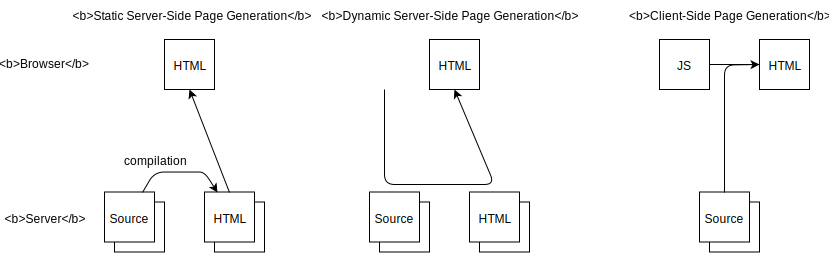
\includegraphics{../../files/dynamic-alternatives.svg}

As browsers and JavaScript became more powerful, the balance shifted
toward \protect\hyperlink{g:client-side-page-generation}{client-side
page generation}. In this model, the browser fetches data from one or
more servers and feeds that data to a JavaScript library that generates
HTML in the browser for display. This allows the
\protect\hyperlink{g:client}{client} to decide how best to render data,
which is increasingly important as phones and tablets take over from
desktop and laptop computers. It also moves the computational burden off
the server and onto the client device, which lowers the cost of
providing data.

Many, many JavaScript frameworks for client-side page generation have
been created, and more are probably being developed right now. We have
chosen \href{https://reactjs.org/}{React} because it is freely
available, widely used, well documented, simpler than many alternatives,
and has a cool logo. Its central design principles are:

\begin{enumerate}
\tightlist
\item
  Page creators use functions to describe the HTML they want.
\item
  They then let React decide which functions to run when data changes.
\end{enumerate}

We will show how to use it in pure JavaScript, then introduce a tool
called JSX that simplifies things.

\subsubsection{Hello, World}\label{s:dynamic-hello}

Let's begin by saying hello:

\begin{verbatim}
<!DOCTYPE html>
<html>
  <head>
    <meta charset="utf-8">
    <title>Hello React</title>
    <script src="https://fb.me/react-15.0.1.js"></script>
    <script src="https://fb.me/react-dom-15.0.1.js"></script>
  </head>
  <body>
    <div id="app">
      <!-- this is filled in -->
    </div>
    <script>
      ReactDOM.render(
        React.DOM.h1(null, "Hello React"),
        document.getElementById("app")
      )
    </script>
  </body>
</html>
\end{verbatim}

The \texttt{head} of the page loads two React libraries from the web; we
will use locally-installed libraries later. The \texttt{body} contains a
\texttt{div} with an ID to make it findable. When our script runs, React
will put the HTML it generates into this \texttt{div}.

The script itself create an \texttt{h1} with the text ``Hello, React''
using \texttt{React.DOM.h1}, then finds the document element whose ID is
\texttt{"app"} and uses \texttt{ReactDOM.render} to insert the former
into the latter. This alters the representation of the page in memory,
not the source of the page on disk; if we want to inspect the HTML, we
have to do so in the browser. Finally, we put the script at the bottom
of the page so that the browser will have turned the HTML into a DOM
tree in memory before the script runs. We will come back and fix this
later.

\begin{quote}
\textbf{Inspection Tools}

If you are using the Firefox browser, you can open the developer tools
pane by going to the main menu and selecting
\texttt{Tools...\ Web\ Developer...\ Toggle\ Tools}. A tabbed display
will open in the bottom of your page; choose \texttt{Inspector} to view
the content of your page and page's CSS. As you move your mouse around
the page itself, corresponding structural elements will be highlighted.
It's actually pretty cool\ldots{}
\end{quote}

The first parameter to \texttt{React.DOM.h1} is \texttt{null} in the
example above, but it can more generally be an object that specifies the
attributes we want the newly-created node to have. There are a few
quirks in this---for example, we have to use \texttt{fontStyle} rather
than \texttt{font-style} so that the attribute object's keys look like
legal JavaScript variables---but the mechanism is surprisingly easy to
use:

\begin{verbatim}
  <body>
    <div id="app"></div>
    <script>
      const attributes = {
        'style': {
          'background': 'pink',
          'fontStyle': 'italic'
        }
      }
      ReactDOM.render(
        React.DOM.h1(attributes, "Hello Stylish"),
        document.getElementById("app")
      )
    </script>
  </body>
\end{verbatim}

\subsubsection{JSX}\label{s:dynamic-jsx}

Writing nested functions is a clumsy way to write HTML, so most React
programmers use a tool called
\href{https://reactjs.org/docs/introducing-jsx.html}{JSX} that
translates HTML into JavaScript function calls. And yes, those
JavaScript function calls then produce HTML---it's a funny world. Here's
an example:

\begin{verbatim}
<!DOCTYPE html>
<html>
  <head>
    <meta charset="utf-8">
    <title>Hello JSX</title>
    <script src="https://fb.me/react-15.0.1.js"></script>
    <script src="https://fb.me/react-dom-15.0.1.js"></script>
    <script src="https://unpkg.com/babel-standalone@6/babel.js"></script>
  </head>
  <body>
    <div id="app"></div>
    <script type="text/babel">
      ReactDOM.render(
        <h1>Hello JSX</h1>,
        document.getElementById('app')
      )
    </script>
  </body>
</html>
\end{verbatim}

Along with the two React libraries, this page includes a tool called
\href{https://babeljs.io/}{Babel} to translate a mixed of HTML and
JavaScript into pure JavaScript. To trigger translation, we add the
attribute \texttt{type="text/babel"} to the \texttt{script} tag.

Why bother? Because as the example above shows, it allows us to write
\texttt{\textless{}h1\textgreater{}Hello\ JSX\textless{}/h1\textgreater{}}
instead of calling a function. More generally, JSX lets us put
JavaScript inside our HTML (inside our JavaScript (inside our HTML)), so
we can (for example) use \texttt{map} to turn a list of strings into an
HTML list:

\begin{verbatim}
  <body>
    <h1>JSX List</h1>
    <div id="app"></div>
    <script type="text/babel">
      const allNames = ['McNulty', 'Jennings', 'Snyder', 'Meltzer', 'Bilas', 'Lichterman']
      ReactDOM.render(
        <ul>{allNames.map((name) => <li>{name}</li> )}</ul>,
        document.getElementById('app')
      )
    </script>
  </body>
\end{verbatim}

We have to use \texttt{map} rather than a loop because whatever code we
run has to return something that can be inserted into the DOM, and
\texttt{for} loops don't return anything. (We could use a loop to build
up a string through repeated concatenation, but \texttt{map} is
cleaner.) And note: we must return exactly one node, because this is one
function call. We will look in the exercises at why the curly braces
immediately inside the \texttt{\textless{}ul\textgreater{}} element are
necessary.

Note also that when we run this, the browser console will warn us that
each list element ought to have a unique \texttt{key} property, because
React wants each element of the page to be selectable. We will add this
later.

\subsubsection{Creating Components}\label{s:dynamic-components}

One of the most powerful features of React is that it lets us create new
components that look like custom HTML tags, but are associated with
functions that we write. React requires the names of these components to
start with a capital letter to differentiate them from regular tags. We
can, for example, define a function \texttt{ListOfNames} to generate our
list of names, then put that element directly in
\texttt{ReactDOM.Render} just as we would put an \texttt{h1} or
\texttt{p}:

\begin{verbatim}
  <body>
    <h1>Create Component</h1>
    <div id="app"></div>
    <script type="text/babel">
      const allNames = ['McNulty', 'Jennings', 'Snyder', 'Meltzer', 'Bilas', 'Lichterman']

      const ListOfNames = () => {
        return (<ul>{allNames.map((name) => <li>{name}</li> )}</ul>)
      }

      ReactDOM.render(
        <ListOfNames />,
        document.getElementById('app')
      )
    </script>
  </body>
\end{verbatim}

What we really want to do, though, is pass parameters to these
components: after all, JSX is turning them into functions, and functions
are far more useful when we can give them data. In React, all the
attributes we put inside the component's tag are passed to our function
in a single \texttt{props} object:

\begin{verbatim}
  <body>
    <h1>Pass Parameters</h1>
    <div id="app"></div>
    <script type="text/babel">
      const allNames = ['McNulty', 'Jennings', 'Snyder', 'Meltzer', 'Bilas', 'Lichterman']

      const ListElement = (props) => (<li id="{props.name}"><em>{props.name}</em></li>)

      ReactDOM.render(
        <ul>{allNames.map((name) => <ListElement name={name} /> )}</ul>,
        document.getElementById('app')
      )
    </script>
  </body>
\end{verbatim}

If you look carefully, you'll see that the \texttt{name} attribute
passed to the use of \texttt{ListElement} becomes the value of
\texttt{prop.names} inside the function that implements
\texttt{ListElement}. This gives us exactly one logical place to do
calculations, set style, etc.

\subsubsection{Developing with Parcel}\label{s:dynamic-parcel}

Putting all of the source for an application in one HTML file is a bad
practice, but we've already seen the race conditions that can arise when
we load JavaScript in a page's header. And what about \texttt{require}
statements? The browser will try to load the required files when those
statements run, but who is going to serve them?

The solution is use a \protect\hyperlink{g:bundler}{bundler} to combine
everything into one big file, and to run a
\protect\hyperlink{g:local-server}{local server} to preview our
application during development. However, this solution brings with it
another problem: which bundler to choose? As with front-end frameworks,
there are many to choose from, and new ones are being added almost
weekly. \href{https://webpack.js.org/}{Webpack} is probably the most
widely used, but it is rather complex, so we will use
\href{https://parceljs.org/}{Parcel}, which is younger and therefore not
yet bloated (but give it time).

To install Parcel, run:

\begin{verbatim}
npm install parcel-bundler
\end{verbatim}

Once it's in place, we can tell it to run one of our test pages like
this:

\begin{verbatim}
node_modules/.bin/parcel serve -p 4000 src/dynamic/pass-parameters.html
\end{verbatim}

\begin{verbatim}
Server running at http://localhost:4000
+ Built in 128ms.
\end{verbatim}

This works because when NPM installs a library in a project's
\texttt{node\_modules} directory, it will sometimes put a runnable
script associated with that library in \texttt{node\_modules/.bin} (note
that it's \texttt{.bin} with a leading \texttt{.}, not \texttt{bin}).
When we ask Parcel to serve up an application, it:

\begin{itemize}
\tightlist
\item
  looks in the named file to find JavaScript,
\item
  looks recursively at what that file loads,
\item
  copies some files into a directory called \texttt{./dist} (which
  stands for ``distribution''), and
\item
  serves the application out of there.
\end{itemize}

Parcel also caches things in \texttt{./.cache} so that it doesn't need
to do redundant work; both directories are normally added to
\texttt{.gitignore}. To learn more about Parcel, see
\href{https://medium.com/codingthesmartway-com-blog/getting-started-with-parcel-197eb85a2c8c}{Sebastian
Eschweiler's quick tutorial}.

It's very common to put tasks like ``run my application'' into NPM's
\texttt{package.json} file, just as older programmers would put
frequently-used commands into a project's Makefile. Look for the section
in \texttt{package.json} whose key is \texttt{"scripts"} and add this:

\begin{verbatim}
  "scripts": {
    "dev": "parcel serve -p 4000",
    ...
  },
\end{verbatim}

We can now use
\texttt{npm\ run\ dev\ -\/-\ src/dynamic/pass-parameters.html}, since
everything after \texttt{-\/-} is passed to the script being run. This
doesn't just save us typing; it also gives other developers a record of
how to use the project. Unfortunately, there is no standard way to add
comments to a JSON file\ldots{}

\begin{quote}
\textbf{Whoops}

Note: if we accidentally specify the name of a directory like
\texttt{src/dynamic} instead of the name of an HTML file, Parcel prints
an error on the console saying ``no entries found''. This happens
because it is trying to read the actual directory structure as if it
were a file.
\end{quote}

\subsubsection{Multiple Files}\label{s:dynamic-multiple}

Now that we can bundle things up, let's move our JSX into
\texttt{app.js} and load that in the \texttt{head} of the page:

\begin{verbatim}
<!DOCTYPE html>
<html>
  <head>
    <meta charset="utf-8">
    <title>Hello Separate</title>
    <script src="https://fb.me/react-15.0.1.js"></script>
    <script src="https://fb.me/react-dom-15.0.1.js"></script>
    <script src="https://unpkg.com/babel-standalone@6/babel.js"></script>
    <script src="app.js"></script>
  </head>
  <body>
    <h1>Hello Separate</h1>
    <div id="app"></div>
  </body>
</html>
\end{verbatim}

For now, the JavaScript in \texttt{app.js} is:

\begin{verbatim}
ReactDOM.render(
  <p>Rendered by React</p>,
  document.getElementById("app")
)
\end{verbatim}

When we load this page we get the \texttt{h1} title but \emph{not} the
paragraph. When we look in the browser console, we see the message:

\begin{verbatim}
Error: _registerComponent(...): Target container is not a DOM element.
\end{verbatim}

This is the same race condition that has bitten us before. After sighing
in frustration and making ourselves another cup of tea, we decide that,
to keep things simple, we will load the script in the body of the page:

\begin{verbatim}
<!DOCTYPE html>
<html>
  <head>
    <meta charset="utf-8">
    <title>Hello Bottom</title>
  </head>
  <body>
    <h1>Hello Bottom</h1>
    <div id="app"></div>
    <script src="./app.js"></script>
  </body>
</html>
\end{verbatim}

More importantly, we will rewrite \texttt{app.js} so that it loads the
libraries it needs, because there's no guarantee that libraries loaded
in \texttt{head} will be available when \texttt{app.js} runs:

\begin{verbatim}
const React = require('react')
const ReactDOM = require('react-dom')

ReactDOM.render(
  <p>Rendered by React</p>,
  document.getElementById('app')
)
\end{verbatim}

We don't have to shut down the server and restart it every time we make
changes like this, because Parcel watches for changes in files and
relaunches itself as needed. Each time it does so, it looks at the
libraries \texttt{app.js} loads and rebundles what it needs: right now,
for example, \texttt{dist/app.ef6b320b.js} is 19930 lines long.

A more modern option than loading in the bottom is to add the
\texttt{async} attribute to the script in the head of the page, which
tells the browser not to do anything with the JavaScript until the page
has finished building:

\begin{verbatim}
<!DOCTYPE html>
<html>
  <head>
    <meta charset="utf-8">
    <title>Hello Parcel</title>
    <script src="./app.js" async></script>
  </head>
  <body>
    <div id="app"></div>
  </body>
</html>
\end{verbatim}

\subsubsection{Exercises}\label{s:dynamic-exercises}

\paragraph{Those Damn Curly Braces}\label{those-damn-curly-braces}

Our list-building example includes this line of code:

\begin{verbatim}
        <ul>{allNames.map((name) => <li>{name}</li> )}</ul>,
\end{verbatim}

Why are the curly braces immediately inside the
\texttt{\textless{}ul\textgreater{}} element necessary? What happens if
you take them out?

\paragraph{Real Data}\label{real-data}

\begin{enumerate}
\tightlist
\item
  Create a file called \texttt{programmers.js} that defines a list of
  JSON objects called \texttt{programmers} with \texttt{firstName} and
  \texttt{lastName} fields for our programmers. (You can search the
  Internet to find their names.)
\item
  Load that file in your page like any other JavaScript file.
\item
  Delete the list \texttt{allNames} from the application and modify it
  to use data from the list \texttt{programmers} instead.
\end{enumerate}

Loading constant data like this is a common practice during testing.

\paragraph{Ordering}\label{ordering}

What happens if you change the order in which the JavaScript files are
loaded in your web page? For example, what happens if you load
\texttt{app.js} \emph{before} you load \texttt{ListElement.js}?

\paragraph{Multiple Targets}\label{multiple-targets}

What happens if your HTML page contains two \texttt{div} elements with
\texttt{id="app"}?

\paragraph{Creating a Component for
Names}\label{creating-a-component-for-names}

Create a new React component that renders a name, and modify the example
to use it instead of always displaying names in
\texttt{\textless{}li\textgreater{}} elements.

\paragraph{Striping}\label{striping}

Suppose we want to render every second list element in italics. (This
would be a horrible design, but once we start creating tables, we might
want to highlight alternate rows in different background colors to make
it easier to read.) Modify the application so that even-numbered list
elements are
\texttt{\textless{}li\textgreater{}\{name\}\textless{}/li\textgreater{}}
and odd-numbered list elements are
\texttt{\textless{}li\textgreater{}\textless{}em\textgreater{}\{name\}\textless{}/em\textgreater{}\textless{}/li\textgreater{}}.
(You may want to use the fact that a \texttt{map} callback can have two
parameters instead of one.)

\textbf{Key Points}

\begin{itemize}
\tightlist
\item
  Older dynamic web sites generated pages on the server.
\item
  Newer dynamic web sites generate pages in the client.
\item
  React is a JavaScript library for client-side page generation that
  represents HTML elements as function calls.
\item
  React replaces page elements with dynamically-generated content in
  memory (not on disk).
\item
  React functions can be customized with elements.
\item
  JSX translates HTML into React function calls so that HTML and
  JavaScript can be mixed freely.
\item
  Use Babel to translate JSX into JavaScript in the browser.
\item
  Define new React components with a pseudo-HTML element and a
  corresponding function.
\item
  Attributes to pseudo-HTML are passed to the JavaScript function as a
  \texttt{props} object.
\end{itemize}

\hypertarget{s:vis}{\subsection{Visualizing Data}\label{s:vis}}

\textbf{Questions}

\begin{itemize}
\tightlist
\item
  How can I visualize data on the web?
\item
  How does loading libraries in the browser differ from loading them on
  the server?
\end{itemize}

Tables and lists are great, but visualizations are often more
effective---if they're well designed and your audience is sighted, that
is. There are even more ways to visualize data in the browser than there
are front-end toolkits for JavaScript. We have chosen to use
\href{http://vega.github.io/}{Vega-Lite}, which is a
\protect\hyperlink{g:declarative-programming}{declarative} framework: as
a user, you specify the data and settings, and let the library take care
of everything else. It doesn't do everything, but it does common things
well and easily, and it interacts nicely with React.

\subsubsection{Vega-Lite}\label{s:vis-vega-lite}

Let's start by creating a skeleton web page to hold our visualization.
For now, we will load Vega, Vega-Lite, and Vega-Embed from the web;
we'll worry about local installation later. We will create a
\texttt{div} to be filled in by the visualization---we don't have to
give it the ID \texttt{vis}, but it's common to do so---and we will
leave space for the script. Our skeleton looks like this:

\begin{verbatim}
<!DOCTYPE html>
<html>
<head>
  <title>Embedding Vega-Lite</title>
  <script src="https://cdnjs.cloudflare.com/ajax/libs/vega/3.0.7/vega.js"></script>
  <script src="https://cdnjs.cloudflare.com/ajax/libs/vega-lite/2.0.1/vega-lite.js"></script>
  <script src="https://cdnjs.cloudflare.com/ajax/libs/vega-embed/3.0.0-rc7/vega-embed.js"></script>
</head>
<body>

  <div id="vis"></div>

  <script type="text/javascript">
  </script>
</body>
</html>
\end{verbatim}

We can now start filling in the script with the beginning of a
visualization specification. This is a blob of
\protect\hyperlink{g:json}{JSON} with certain required fields:

\begin{itemize}
\tightlist
\item
  \texttt{\$schema} identifies the version of the spec being used (as a
  URL).
\item
  \texttt{description} is a comment to remind us what we thought we were
  doing when we created this.
\item
  \texttt{data} is the actual data.
\end{itemize}

\begin{verbatim}
...rest of page as before...
  <script type="text/javascript">
    let spec = {
      "$schema": "https://vega.github.io/schema/vega-lite/v2.0.json",
      "description": "Create data array but do not display anything.",
      "data": {
        "values": [
          {"a": "A", "b": 28},
          {"a": "B", "b": 55},
          {"a": "C", "b": 43},
          {"a": "D", "b": 91},
          {"a": "E", "b": 81},
          {"a": "F", "b": 53},
          {"a": "G", "b": 19},
          {"a": "H", "b": 87},
          {"a": "I", "b": 52}
        ]
      }
    }
  </script>
...rest of page as before...
\end{verbatim}

In this case, we represent a two-dimensional data table as objects with
explicit indices \texttt{"a"} and \texttt{"b"}. We have to do this
because JSON (like JavaScript) doesn't have a native representation of
two-dimensional arrays with row and column headers, because programmers.

Once we have created our spec, we can call \texttt{vegaEmbed} with the
ID of the element that will hold the visualization, the spec, and some
options (which for now we will leave empty):

\begin{verbatim}
    let spec = {
      "$schema": "https://vega.github.io/schema/vega-lite/v2.0.json",
      "description": "Create data array but do not display anything.",
      "data": {
        "values": [
          // ...as above...
        ]
      }
    }
    vegaEmbed("#vis", spec, {})
\end{verbatim}

When we open the page, though, nothing appears, because we haven't told
Vega-Lite \emph{how} to display the data. To do that, we need to add two
more fields to the spec:

\begin{itemize}
\tightlist
\item
  \texttt{mark} specifies the visual element used to show the data
\item
  \texttt{encoding} tells Vega how to map values to marks
\end{itemize}

Here's our updated spec:

\begin{verbatim}
    let spec = {
      "$schema": "https://vega.github.io/schema/vega-lite/v2.0.json",
      "description": "Add mark and encoding for data.",
      "data": {
        "values": [
          // ...as above...
        ]
      },
      "mark": "bar",
      "encoding": {
        "x": {"field": "a", "type": "ordinal"},
        "y": {"field": "b", "type": "quantitative"}
      }
    }
    vegaEmbed("#vis", spec, {})
\end{verbatim}

When we open the page now, we see a bar chart, and feel very proud of
ourselves.

Mark and Encoding

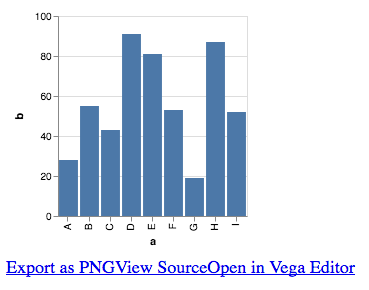
\includegraphics{../../files/vis-mark-encoding.png}

There are also some poorly-styled links for various controls that we're
not going to use. We can fill in the options argument to
\texttt{vegaEmbed} to turn those off:

\begin{verbatim}
    let spec = {
      "$schema": "https://vega.github.io/schema/vega-lite/v2.0.json",
      "description": "Disable control links.",
      "data": {
        // ...as before...
      }
    }
    let options = {
      "actions": {
        "export": false,
        "source": false,
        "editor": false
      }
    }
    vegaEmbed("#vis", spec, options)
\end{verbatim}

We now have the visualization we wanted:

Without Controls

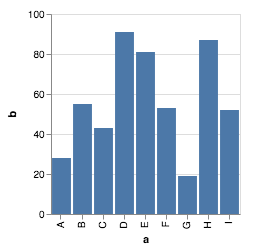
\includegraphics{../../files/vis-disable-controls.png}

Vega-Lite has a \emph{lot} of options: for example, we can use points
and average the Y values. (We will change the X data so that values
aren't distinct in order to show this off, because otherwise averaging
doesn't do much.) In our revised spec, \texttt{x} is now
\texttt{"nominal"} instead of \texttt{"ordinal"} and \texttt{y} has an
extra property \texttt{"aggregate"}, which is set to \texttt{"average"}
(but can be used to specify other
\protect\hyperlink{g:aggregation-function}{aggregation functions}):

\begin{verbatim}
    let spec = {
      "$schema": "https://vega.github.io/schema/vega-lite/v2.0.json",
      "description": "Disable control links.",
      "data": {
        "values": [
          {"a": "P", "b": 19},
          {"a": "P", "b": 28},
          {"a": "P", "b": 91},
          {"a": "Q", "b": 55},
          {"a": "Q", "b": 81},
          {"a": "Q", "b": 87},
          {"a": "R", "b": 43},
          {"a": "R", "b": 52},
          {"a": "R", "b": 53}
        ]
      },
      "mark": "point",
      "encoding": {
        "x": {"field": "a", "type": "nominal"},
        "y": {"field": "b", "type": "quantitative", "aggregate": "average"}
      }
    }
    let options = {
      ...disable controls as before...
    }
    vegaEmbed("#vis", spec, options)
\end{verbatim}

Aggregating and Using Points

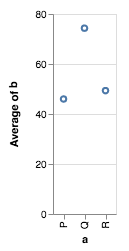
\includegraphics{../../files/vis-aggregate-points.png}

\subsubsection{Local Installation}\label{s:vis-vega-local}

Loading Vega from a \protect\hyperlink{g:cdn}{Content Delivery Network}
(CDN) reduces the load on our server, but prevents offline development.
Since we want to be able to work when we're disconnected, let's load
from local files.

Step 1 is to slim down our HTML file so that it only loads our
application:

\begin{verbatim}
<!DOCTYPE html>
<html>
  <head>
    <title>Load Vega from a File</title>
    <meta charset="utf-8">
    <script src="app.js" async></script>
  </head>
  <body>
    <div id="vis"></div>
  </body>
</html>
\end{verbatim}

In step 2, we \texttt{npm\ install\ vega\ vega-lite\ vega-embed} and
\texttt{require(\textquotesingle{}vega-embed\textquotesingle{})} in
\texttt{app.js}:

\begin{verbatim}
const vegaEmbed = require('vega-embed')

const spec = {
  // ...as before...
}

const options = {
  // ...as before...
}

vegaEmbed("#vis", spec, options)
\end{verbatim}

We launch this with Parcel via our saved \texttt{npm\ run} command:

\begin{verbatim}
npm run dev -- src/vis/react-01/index.html
\end{verbatim}

But nothing appears when we open \texttt{http://localhost:4000} in our
browser. Looking in the browser console, we see a message telling us
that \texttt{vegaEmbed} is not a function.

What we have tripped over is something that's still painful in 2018. The
old method of getting libraries is \texttt{require}, and that's still
what Node supports as of Version 10.9.0. The new standard is
\texttt{import}, which allows a module to define a default value so that
\texttt{import\ \textquotesingle{}something\textquotesingle{}} gets a
function, a class, or whatever. This is really handy, but
\texttt{require} doesn't work that way.

Using Node on the command line, we can either add the
\texttt{-\/-experimental-modules} flag or rename our files with a
\texttt{.mjs} extension, both of which are annoying. Alternatively, we
can get the thing we want by accessing \texttt{.default} during import,
or by referring to \texttt{vegaEmbed.default} when we call it. These
choices are also annoying, but after a bit of fiddling and cursing, we
decide to make the fix as the library is loaded:

\begin{verbatim}
const vegaEmbed = require('vega-embed').default

// ...as before...
\end{verbatim}

The third option is to use \texttt{import} where we can and fix the
\texttt{require} statements in the server-side code when Node is
upgraded. We can call the thing we import anything we want, but we will
stick to \texttt{vegaEmbed} for consistency with previous examples:

\begin{verbatim}
import vegaEmbed from 'vega-embed'

// ...as before...
\end{verbatim}

If we do this, the bundled file is 74.5K lines of JavaScript, but at
least it's all in one place for distribution.

\subsubsection{Exercises}\label{s:vis-exercises}

\paragraph{Binned Scatterplots}\label{binned-scatterplots}

Vega-Lite can create
\href{https://vega.github.io/vega-lite/examples/circle_binned.html}{binned
scatterplots} in which the sizes of markers indicate how many values
were put in each bin. Modify the aggregating scatterplot shown above so
that values are binned in this way.

\paragraph{Grouped Bar Charts}\label{grouped-bar-charts}

Vega-Lite can display
\href{https://vega.github.io/vega-lite/examples/bar_grouped.html}{grouped
bar charts} as well as simple ones. Find or create a simple data set and
construct a grouped bar chart. How impressed will your supervisor, your
committee, or a future employee be by your chosen color scheme?

\paragraph{Limits of Declarative
Programming}\label{limits-of-declarative-programming}

Look at Vega-Lite's
\href{https://vega.github.io/vega-lite/examples/}{example gallery} and
identify one kind of plot or transformation you've used or seen that
\emph{isn't} included there. Do you think this is because they just
haven't gotten around to it yet, or is there something about that plot
or transformation that doesn't lend itself to Vega-Lite's declarative
model?

\paragraph{Working With Arrays}\label{working-with-arrays}

Vega-Lite is built on top of a visualization toolkit called
\href{https://d3js.org/}{D3}, which includes
\href{https://github.com/d3/d3-array}{a library for manipulating
arrays}. Write a small application that generates 1000 random values
using \texttt{Math.random} and reports the mean, standard deviation, and
quartiles. (You may also want to create a histogram showing the
distribution of values.)

\textbf{Key Points}

\begin{itemize}
\tightlist
\item
  Vega-Lite is a simple way to build common visualizations.
\item
  Vega-Lite is declarative: the user creates a data structure describing
  what they want, and the library creates the visualization.
\item
  A Vega-List specification contains a schema identifier, a description,
  data, marks, and encodings.
\item
  The overall layout of a Vega-Lite visualization can be controlled by
  setting options.
\item
  Some applications will use \texttt{require} for server-side code and
  \texttt{import} for client-side code.
\end{itemize}

\hypertarget{s:promises}{\subsection{Promises}\label{s:promises}}

\textbf{Questions}

\begin{itemize}
\tightlist
\item
  How does JavaScript implement delayed computation?
\item
  Is there an easier way to handle delayed computation?
\item
  How can a program wait for many promises to complete, or for one
  promise in a set to complete?
\item
  Is there an even easier way to manage all of this?
\end{itemize}

By now we have got used to providing callback functions as arguments to
other functions. Callbacks quickly become complicated because of:

\begin{itemize}
\tightlist
\item
  Nesting: a delayed calculation may need the result of a delayed
  calculation that needs\ldots{}
\item
  Error handling: who notices and takes care of errors? (This is often a
  problem in real life too.)
\end{itemize}

For example, suppose we want to turn a set of CSV files into HTML pages.
The inputs to our function are the name of a directory that contains one
or more CSV files and the name of an output directory; the desired
results are that the output directory is created if it doesn't already
exist, that one HTML file is created for each CSV file, that any HTML
files in the directory that \emph{don't} correspond to CSV files are
removed, and that an index page is created with links to all the pages.

We can do this with synchronous operations, but that's not the
JavaScript way (by which we mean that doing it that way won't introduce
you to tools we're going to need later). We can also try doing it with
callbacks, but:

\begin{itemize}
\tightlist
\item
  we can't create the output directory until the existing one has been
  emptied;
\item
  can't generate the HTML pages until the output directory has been
  re-created; and
\item
  we can't generate the index page until the CSV files have been
  processed.
\end{itemize}

Instead of a tangled nest of callbacks, it's better to use
\protect\hyperlink{g:promise}{promises}, and then to use \texttt{async}
and \texttt{await} to make things even easier. JavaScript offers three
mechanisms because its developers have invented better ways to do things
as the language has evolved, but the simple high-level ideas often don't
make sense unless you understand how they work. (This too is often a
problem in real life.)

\subsubsection{The Execution Queue}\label{s:promises-queue}

In order for any of what follows to make sense, it's vital to understand
JavaScript's \protect\hyperlink{g:event-loop}{event loop}, a full
explanation of which can be found
\href{https://nodejs.org/en/docs/guides/event-loop-timers-and-nexttick/}{here}.
Most functions execute in order:

\begin{verbatim}
[1000, 1500, 500].forEach(t => {
  console.log(t)
})
\end{verbatim}

\begin{verbatim}
1000
1500
500
\end{verbatim}

However, a handful of built-in functions delay execution: instead of
running right away, they add a callback to a list that the JavaScript
interpreter uses to keep track of things that want to be run. When one
task finishes, the interpreter takes the next one from this queue and
runs it.

\texttt{setTimeout} is one of the most widely used functions of this
kind. Here it is in operation:

\begin{verbatim}
[1000, 1500, 500].forEach(t => {
  console.log(`about to setTimeout for ${t}`)
  setTimeout(() => {console.log(`inside timer handler for ${t}`)}, t)
})
\end{verbatim}

\begin{verbatim}
about to setTimeout for 1000
about to setTimeout for 1500
about to setTimeout for 500
inside timer handler for 500
inside timer handler for 1000
inside timer handler for 1500
\end{verbatim}

That's not surprising: if we ask JavaScript to delay execution,
execution is delayed. What may be surprising is that setting a timeout
of zero also defers execution:

\begin{verbatim}
const values = [1000, 1500, 500]
console.log('starting...')
values.forEach(t => {
  console.log(`about to setTimeout for ${t}`)
  setTimeout(() => {console.log(`inside timer handler for ${t}`)}, 0)
})
console.log('...finishing')
\end{verbatim}

\begin{verbatim}
starting...
about to setTimeout for 1000
about to setTimeout for 1500
about to setTimeout for 500
...finishing
inside timer handler for 1000
inside timer handler for 1500
inside timer handler for 500
\end{verbatim}

Here's what the run queue looks like just before the program prints
\texttt{...finishing}:

Run Queue

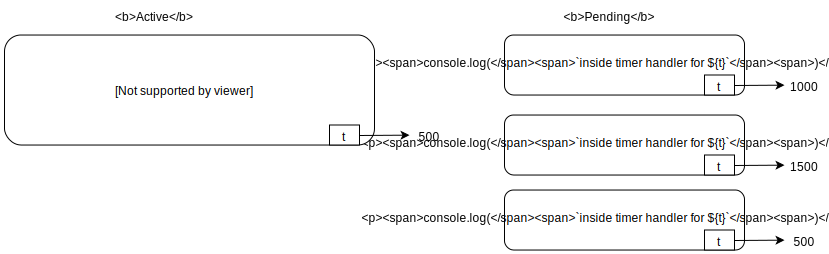
\includegraphics{../../files/promises-queue.svg}

We can use \texttt{setTimeout} to build a generic non-blocking function:

\begin{verbatim}
const nonBlocking = (callback) => {
  setTimeout(callback, 0)
}

['a', 'b', 'c'].forEach(val => {
  console.log(`about to do nonBlocking for ${val}`)
  nonBlocking(() => console.log(`inside callback for ${val}`))
})
\end{verbatim}

\begin{verbatim}
about to do nonBlocking for a
about to do nonBlocking for b
about to do nonBlocking for c
inside callback for a
inside callback for b
inside callback for c
\end{verbatim}

Why bother doing this? Because we may want to give something else a
chance to run. In particular, file I/O and anything involving a network
request are incredibly slow from a computer's point of view.
\href{http://exple.tive.org/blarg/2018/08/15/time-dilation/}{If a single
CPU cycle was one second long}, then getting data from RAM would take
several minutes, getting it from a solid-state disk would take six to
eight days, and getting it over the network is the equivalent of eight
years. Rather than wasting that time, JavaScript is designed to let us
(or our browser) switch tasks and do something else.

Using a timeout of zero is a clever trick, but Node provides another
function called \texttt{setImmediate} to do this for us. (There is also
\texttt{process.nextTick}, which doesn't do quite the same thing. You
should probably not use it.)

\begin{verbatim}
['a', 'b', 'c'].forEach(val => {
  console.log(`about to do setImmediate for ${val}`)
  setImmediate(() => console.log(`inside immediate handler for ${val}`))
})
\end{verbatim}

\begin{verbatim}
about to do setImmediate for a
about to do setImmediate for b
about to do setImmediate for c
inside immediate handler for a
inside immediate handler for b
inside immediate handler for c
\end{verbatim}

\subsubsection{Promises}\label{s:promises-promises}

Recent versions of JavaScript encourage programmers to use
\protect\hyperlink{g:promise}{promises} to manage delayed actions. For
example, if we want to find the size of a file, we can write this:

\begin{verbatim}
const fs = require('fs-extra')
fs.stat('moby-dick.txt').then((stats) => console.log(stats.size))
\end{verbatim}

\begin{verbatim}
1276201
\end{verbatim}

\texttt{fs-extra.stat} will eventually produce some statistics about the
file, but this will take a while, so \texttt{fs-extra.stat} returns a
object of the class \texttt{Promise} right away. \texttt{Promise} has a
method \texttt{then} that takes a callback as an argument and stores it
in the promise object. When the \texttt{stat} call completes, the
remembered callback is called, and passed yet another object with
statistics about the file (including its size).

To understand this a little better, let's create our own promise to
fetch a file from the web:

\begin{verbatim}
const fetch = require('node-fetch')

const prom = new Promise((resolve, reject) => {
  fetch('https://api.nasa.gov/neo/rest/v1/feed?api_key=DEMO_KEY&start_date=2018-08-20')
  .then((response) => {
    if (response.status === 200) {
      resolve('fetched page successfully')
    }
  })
}).then((message) => console.log(message))
\end{verbatim}

This code constructs a new \texttt{Promise} object. The constructor
takes one argument; this must be a callback function of two arguments,
which by convention are called \texttt{resolve} and \texttt{reject}.
Inside the body of the callback, we call \texttt{resolve} to return a
value if and when everything worked as planned. That value is then
passed to the \texttt{then} method of the \texttt{Promise}.

This may seem a roundabout way of doing things, but it solves several
problems at once. The first and most important is error handling: if
something goes wrong inside the callback passed to \texttt{Promise}'s
constructor, we can call \texttt{reject} instead of \texttt{resolve}.
Just as \texttt{then} handles whatever we pass to \texttt{resolve},
\texttt{Promise} defines a method called \texttt{catch} to handle
whatever is passed to \texttt{reject}. We can therefore build a slightly
more robust version of our data fetcher that will report something
sensible if we mis-type a year as \texttt{2108}:

\begin{verbatim}
const fetch = require('node-fetch')

new Promise((resolve, reject) => {
  fetch('https://api.nasa.gov/neo/rest/v1/feed?api_key=DEMO_KEY&start_date=20-08-2108')
  .then((response) => {
    if (response.status === 200) {
      resolve('fetched page successfully')
    }
    else {
      reject(Error(`got HTTP status code ${response.status}`))
    }
  })
}).then((message) => console.log(message))
.catch((error) => console.log(error.message))
\end{verbatim}

\begin{verbatim}
got HTTP status code 400
\end{verbatim}

(Note that we didn't assign our Promise object to a variable in the
example above. We can create promises on the fly if we need them only to
define behaviour on successful completion/exception and won't need to
refer to them again later.) What makes this all work is that a promise
is an object. Here's what's in memory just after this promise has been
created:

Promises as Objects (after creation)

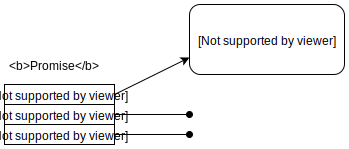
\includegraphics{../../files/promises-object-a.svg}

There are a lot of arrows in this diagram, but they all serve a purpose:

\begin{itemize}
\tightlist
\item
  The promise has three fields: the initial action (which is the
  callback passed to the constructor), the action to be taken if
  everything succeeds, and the action to be taken if there's an error.
\item
  The success and error actions are empty, because the initial action
  hasn't executed yet.
\end{itemize}

Once the promise is created, the program calls its \texttt{then} and
\texttt{catch} methods in that order, giving each a callback. This
happens \emph{before} the callback passed to the constructor (i.e., the
initial action) is executed, and leaves the promise in this state:

Promises as Objects (after then and catch)

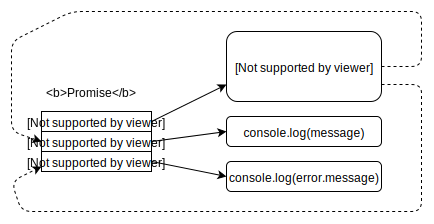
\includegraphics{../../files/promises-object-b.svg}

Calling \texttt{then} and \texttt{catch} assigns callbacks to the
success action and error action members of the promise object. Those
methods are then passed into the initial action callback as
\texttt{resolve} and \texttt{reject}, i.e., if \texttt{resolve} is
called because the page was fetched successfully, what's actually called
is the promise's success action, which is the callback that was given to
\texttt{then}. If \texttt{reject} is called, on the other hand, it
triggers execution of the error action, which is the callback that was
passed to \texttt{catch}.

Yes, this is complicated---so complicated that another layer (which we
will look at \protect\hyperlink{s:promises-async-await}{soon}) has been
added to JavaScript to hide these details. Without this complexity,
though, it's extremely difficult to handle errors from delayed
computations. If we try this, using JavaScript's
\texttt{try\ \{...\}\ catch\ \{...\}} syntax for handling exceptions:

\begin{verbatim}
const fetch = require('node-fetch')

try {
  fetch('https://api.nasa.gov/neo/rest/v1/feed?api_key=DEMO_KEY&start_date=20-08-2108')
}
catch (err) {
  console.log(err)
}
\end{verbatim}

then the error message won't appear because the call to \texttt{fetch}
doesn't raise an exception right away.

Going back to the \texttt{fs-extra.stat} example above, what if we want
to process multiple files, e.g., calculate their total size? We could
write a loop:

\begin{verbatim}
const fs = require('fs-extra')

let total_size = 0
const files = ['jane-eyre.txt', 'moby-dick.txt', 'life-of-frederick-douglass.txt']
for (let fileName of files) {
  fs.stat(fileName).then((stats) => {
    total_size += stats.size
  })
}
console.log(total_size)
\end{verbatim}

but this doesn't work: the \texttt{stat} in each iteration is executed
asynchronously, so the loop finishes and the script prints a total size
of zero before any of the promised code has run.

Plan B is to chain the promises together to ensure that each executes
only after the last has resolved:

\begin{verbatim}
const fs = require('fs-extra')

let total_size = 0
new Promise((resolve, reject) => {
  fs.stat('jane-eyre.txt').then((jeStats) => {
    fs.stat('moby-dick.txt').then((mdStats) => {
      fs.stat('life-of-frederick-douglass.txt').then((fdStats) => {
        resolve(jeStats.size + mdStats.size + fdStats.size)
      })
    })
  })
}).then((total) => console.log(total))
\end{verbatim}

but this obviously doesn't handle an arbitrary number of files, since we
have to write one level of nesting for each file. It's also potentially
inefficient, since we could be waiting for one promise to complete while
other promises further down are ready to be processed.

The answer is \texttt{Promise.all}, which returns an array of results
from completed promises after all of them have resolved. The order of
results corresponds to the order of the promises in the input array,
which makes processing straightforward:

\begin{verbatim}
const fs = require('fs-extra')

let total_size = 0
const files = ['jane-eyre.txt', 'moby-dick.txt', 'life-of-frederick-douglass.txt']
Promise.all(files.map(f => fs.stat(f))).
  then(stats => stats.reduce((total, s) => {return total + s.size}, 0)).
  then(console.log)
\end{verbatim}

\begin{verbatim}
2594901
\end{verbatim}

We can also use \texttt{Promise.race}, which takes an array of promises
and returns the result of the first one to complete.

\subsubsection{Using Promises}\label{s:promises-usage}

Promises don't really make sense until we start to use them, so let's
try counting the number of lines in a set of files that are larger than
a specified threshold. This is a slightly complex example but we will go
through and build it up step-by-step. Step 1 is to find the input files:

\begin{verbatim}
const fs = require('fs-extra')
const glob = require('glob-promise')

const srcDir = process.argv[2]

glob(`${srcDir}/**/*.txt`)
  .then(files => console.log('glob', files))
  .catch(error => console.error(error))
\end{verbatim}

\begin{verbatim}
glob [ './common-sense.txt',
  './jane-eyre.txt',
  './life-of-frederick-douglass.txt',
  './moby-dick.txt',
  './sense-and-sensibility.txt',
  './time-machine.txt' ]
\end{verbatim}

Step 2 is to get the status of each file. This approach doesn't work
because \texttt{fs.stat} is delayed:

\begin{verbatim}
// ...imports and arguments as before...

glob(`${srcDir}/**/*.txt`)
  .then(files => files.map(f => fs.stat(f)))
  .then(files => console.log('glob + files.map/stat', files))
  .catch(error => console.error(error))
\end{verbatim}

\begin{verbatim}
glob + files.map/stat [ Promise { <pending> },
  Promise { <pending> },
  Promise { <pending> },
  Promise { <pending> },
  Promise { <pending> },
  Promise { <pending> } ]
\end{verbatim}

Step 3 is to use \texttt{Promise.all} to wait for all these promises to
resolve:

\begin{verbatim}
// ...imports and arguments as before...

glob(`${srcDir}/**/*.txt`)
  .then(files => Promise.all(files.map(f => fs.stat(f))))
  .then(files => console.log('glob + Promise.all(files.map/stat)', files))
  .catch(error => console.error(error))
\end{verbatim}

\begin{verbatim}
glob + Promise.all(files.map/stat) [ Stats {
    dev: 16777220,
    mode: 33188,
    ...more information... },
    ...five more Stats objects...
]
\end{verbatim}

In step 4, we remember that we need to keep track of the names of the
files we are looking at, so we need to write our own function that
returns an object with two keys (one for the filename, and one for the
stats). As described \protect\hyperlink{s:pages}{previously}, the
notation \texttt{\{a,\ b\}} produces an object
\texttt{\{"a":\ a,\ "b",\ b\}}:

\begin{verbatim}
// ...imports and arguments as before...

const statPair = (filename) => {
  return new Promise((resolve, reject) => {
    fs.stat(filename)
      .then(stats => resolve({filename, stats}))
      .catch(error => reject(error))
  })
}

glob(`${srcDir}/**/*.txt`)
  .then(files => Promise.all(files.map(f => statPair(f))))
  .then(files => console.log('glob + Promise.all(files.map/statPair)', files))
  .catch(error => console.error(error))
\end{verbatim}

\begin{verbatim}
glob + Promise.all(files.map/statPair) [ { filename: './common-sense.txt',
    stats:
     Stats {
       dev: 16777220,
       mode: 33188,
       ...more information... }
     },
     ...five more (filename, Stats) pairs...
]
\end{verbatim}

Step 5 is to make sure that we're only working with files more than
100,000 characters long:

\begin{verbatim}
// ...imports and arguments as before...

glob(`${srcDir}/**/*.txt`)
  .then(files => Promise.all(files.map(f => statPair(f))))
  .then(files => files.filter(pair => pair.stats.size > 100000))
  .then(files => Promise.all(files.map(f => fs.readFile(f.filename, 'utf8'))))
  .then(contents => console.log('...readFile', contents.map(c => c.length)))
  .catch(error => console.error(error))
\end{verbatim}

\begin{verbatim}
...readFile [ 148134, 1070331, 248369, 1276201, 706124, 204492 ]
\end{verbatim}

In step 6, we split each file's content into lines and count:

\begin{verbatim}
// ...imports and arguments as before...

const countLines = (text) => {
  return text.split('\n').length
}

glob(`${srcDir}/**/*.txt`)
  .then(files => Promise.all(files.map(f => statPair(f))))
  .then(files => files.filter(pair => pair.stats > 100000))
  .then(files => Promise.all(files.map(f => fs.readFile(f.filename, 'utf8'))))
  .then(contents => contents.map(c => countLines(c)))
  .then(lengths => console.log('lengths', lengths))
  .catch(error => console.error(error))
\end{verbatim}

\begin{verbatim}
lengths [ 2654, 21063, 4105, 22334, 13028, 3584 ]
\end{verbatim}

There's a lot going on in the example above but the important points
are:

\begin{itemize}
\tightlist
\item
  Promises always return another \texttt{Promise} object.
\item
  This allows us to chain multiple \texttt{then} calls.
\item
  This chain is formed of processes that will each wait to run until
  their predecessor has completed.
\item
  A single \texttt{catch} method works to handle exceptions raised by
  \emph{any} of the previous steps.
\end{itemize}

\hypertarget{s:promises-async-await}{\subsubsection{\texorpdfstring{\texttt{async}
and \texttt{await}}{async and await}}\label{s:promises-async-await}}

Programmers are never content to leave well enough alone, so the latest
version of JavaScript offers yet another tool for managing asynchronous
computation. As we saw above, the result of \texttt{Promise.then} is
another promise, which allows us to create long chains of
\texttt{.then(...).then(...).then(...)} calls. It works, but it isn't
the most readable of notations and has been known to create a feeling of
being trapped.

We can avoid this using two new keywords, \texttt{async} and
\texttt{await}. \texttt{async} tells JavaScript that a function is
asynchronous, i.e., that it might want to wait for something to
complete. Inside an asynchronous function, \texttt{await} tells
JavaScript to act as if it had waited for something to finish. We use
the two together like this:

\begin{verbatim}
const fs = require('fs-extra')

const statPairAsync = async (filename) => {
  const stats = await fs.stat(filename)
  return {filename, stats}
}

statPairAsync('moby-dick.txt').then((white_whale) => console.log(white_whale.stats))
\end{verbatim}

An \texttt{async} function still returns a \texttt{Promise}, but we can
chain those promises together with other \texttt{async} functions using
\texttt{await}, which collects the result returned by a resolved
promise. As before, we can use \texttt{.catch} to handle any errors
thrown.

Let's use these to convert the complete example from the previous
section:

\begin{verbatim}
const fs = require('fs-extra')
const glob = require('glob-promise')

const statPairAsync = async (filename) => {
  const stats = await fs.stat(filename)
  return {filename, stats}
}

const countLines = (text) => {
  return text.split('\n').length
}

const processFiles = async (globpath) => {
  const filenames = await glob(globpath)
  const pairs = await Promise.all(filenames.map(f => statPairAsync(f)))
  const filtered = pairs.filter(pair => pair.stats.size > 100000)
  const contents = await Promise.all(filtered.map(f => fs.readFile(f.filename, 'utf8')))
  const lengths = contents.map(c => countLines(c))
  console.log(lengths)
}

const srcDir = process.argv[2]

processFiles(`${srcDir}/**/*.txt`)
  .catch(e => console.log(e.message))
\end{verbatim}

Using \texttt{async} and \texttt{await} lets us avoid long \texttt{then}
chains; unless and until JavaScript allows us to define operators like
R's \texttt{\%\textgreater{}\%} pipe operator, they are probably the
easiest way to write readable code. Note, though, that we can only use
\texttt{await} inside \texttt{async} functions: JavaScript will report a
syntax error if we use them elsewhere. In particular, we cannot use them
interactively unless we wrap whatever we want to do in a wee function.

\subsubsection{Exercises}\label{s:promises-exercises}

\paragraph{What's Going On?}\label{whats-going-on}

This code runs fine:

\begin{verbatim}
[500, 1000].forEach(t => {
  console.log(`about to setTimeout for ${t}`)
  setTimeout(() => {console.log(`inside timer handler for ${t}`)}, 0)
})
\end{verbatim}

but this code fails:

\begin{verbatim}
console.log('starting...')
[500, 1000].forEach(t => {
  console.log(`about to setTimeout for ${t}`)
  setTimeout(() => {console.log(`inside timer handler for ${t}`)}, 0)
})
\end{verbatim}

Why?

\paragraph{A Stay of Execution}\label{a-stay-of-execution}

Insert
\texttt{console.log(\textquotesingle{}This\ is\ a\ sharp\ Medicine,\ but\ it\ is\ a\ Physician\ for\ all\ diseases\ and\ miseries.\textquotesingle{})}
in the appropriate place in the code block below so that the output
reads

\begin{verbatim}
Waiting...
This is a sharp Medicine, but it is a Physician for all diseases and miseries.
Waiting...
Finished.
\end{verbatim}

\begin{verbatim}
const holdingMessage = () => {
  console.log('Waiting...')
}

const swingAxe = () => {
  setTimeout(() => {
    holdingMessage()
    console.log('Finished.')
  }, 100)
  holdingMessage()
}

swingAxe()
\end{verbatim}

\paragraph{A Synchronous or
Asynchronous?}\label{a-synchronous-or-asynchronous}

Which of these functions would you expect to be asynchronous? How can
you tell? Does it matter? And, if so, what is a good strategy to find
out for sure if a function is asynchronous?

\begin{enumerate}
\tightlist
\item
  \texttt{findNearestTown(coords)}: given a set of coordinates
  (\texttt{coords}) in Brazil, looks up and returns the name of the
  nearest settlement with an estimated population greater than 5000. The
  function throws an error if \texttt{coords} fall outside Brazil.
\item
  \texttt{calculateSphereVolume(r)}: calculates and returns the volume
  of a sphere with radius \texttt{r}.
\item
  \texttt{calculateRoute(A,B)}: returns all possible routes by air
  between airports \texttt{A} and \texttt{B}, including direct routes
  and those with no more than 2 transfers.
\end{enumerate}

\paragraph{Handling Exceptions}\label{handling-exceptions}

What (if any) output would you expect to see in the console when the
code below is executed?

\begin{verbatim}
const checkForBlanks = (inputValue) => {
  return new Promise((resolve, reject) => {
    if (inputValue === '') {
      reject(Error("Blank values are not allowed"))
    } else {
      resolve(inputValue)
    }
  })
}

new Promise((resolve, reject) => {
  setTimeout(() => {
    reject(Error('Timed out!'))
  }, 1000)
  resolve('')
}).then(
  output => checkForBlanks(output), error => console.log(error.message)).then(
    checkedOutput => console.log(checkedOutput)).catch(
      error => console.log(error.message))
\end{verbatim}

\begin{enumerate}
\tightlist
\item
  \texttt{Timed\ out!}
\item
  blank output
\item
  \texttt{Blank\ values\ are\ not\ allowed}
\item
  a new \texttt{Promise} object
\end{enumerate}

\paragraph{Empty Promises}\label{empty-promises}

Fill in the blanks (\texttt{\_\_\_})in the code block below so that the
function returns \texttt{Array{[}7,\ 8,\ 2,\ 6,\ 5{]}}.

\begin{verbatim}
const makePromise = (someInteger) => {
  return ___ Promise((resolve, reject) => {
    setTimeout(___(someInteger), someInteger * 1000)
  })
}
Promise.___([makePromise(7), makePromise(___), makePromise(2), makePromise(6), makePromise(5)]).then(
  numbers => ___(numbers))
\end{verbatim}

Now adapt the function so that it returns only \texttt{2}. (Hint: you
can achieve this by changing only one of the blank fields.)

\paragraph{\texorpdfstring{\texttt{async}, Therefore I
Am}{async, Therefore I Am}}\label{async-therefore-i-am}

Using \texttt{async} and \texttt{await}, convert the completed function
above into an asynchronous function with the same behaviour and output.
Do you find your solution easier to read and follow than the original
version? Do you think that that is only because you wrote this version?

\textbf{Key Points}

\begin{itemize}
\tightlist
\item
  JavaScript keeps an execution queue for delayed computations.
\item
  Use promises to manage delayed computation instead of raw callbacks.
\item
  Use a callback with two arguments to handle successful completion
  (resolve) and unsuccessful completion (reject) of a promise.
\item
  Use \texttt{then} to express the next step after successful completion
  and \texttt{catch} to handle errors.
\item
  Use \texttt{Promise.all} to wait for all promises in a list to
  complete and \texttt{Promise.race} to wait for the first promise in a
  set to complete.
\item
  Use \texttt{await} to wait for the result of a computation.
\item
  Mark functions that can be waited on with \texttt{async}.
\end{itemize}

\hypertarget{s:interactive}{\subsection{Interactive
Sites}\label{s:interactive}}

\textbf{Questions}

\begin{itemize}
\tightlist
\item
  How do I tell the browser what to do when someone clicks a button?
\item
  How should I structure my code to make interactions manageable?
\item
  How can a web application get data from a server?
\item
  How does modern JavaScript handle asynchronous operations?
\end{itemize}

Browsers allow us to define \protect\hyperlink{g:event-handler}{event
handlers} to specify what to do in response to an externally-triggered
action, such as a page loading or a user pressing a button. These event
handlers are just callback functions that are (usually) given an
\protect\hyperlink{g:event-object}{event object} containing information
about what happened, and while we can write them in pure JavaScript,
they're even easier to build in React.

Let's switch back to single-page examples for a moment to show how we
pass a callback function as a specifically-named property of the thing
whose behavior we are specifying. (Don't forget to load the required
libraries in the HTML header, like we did
\protect\hyperlink{s:dynamic}{earlier}.)

\begin{verbatim}
  <body>
    <div id="app"></div>
    <script type="text/babel">
      let counter = 0
      const sayHello = (event) => {
        counter += 1
        console.log(`Hello, button: ${counter}`)
      }

      ReactDOM.render(
        <button onClick={sayHello}>click this</button>,
        document.getElementById("app")
      )
    </script>
  </body>
\end{verbatim}

As its name suggests, a button's \texttt{onClick} handler is called
whenever the button is clicked. Here, we are telling React to call
\texttt{sayHello}, which adds one to the variable \texttt{counter} and
then prints its value along with a greeting message.

Global variables and functions are a poor way to structure code. It's
far better to define the component as a class and then use a method as
the event handler:

\begin{verbatim}
  <body>
    <div id="app"></div>
    <script type="text/babel">
      class Counter extends React.Component {

        constructor (props) {
          super(props)
          this.state = {counter: 0}
        }

        increment = (event) => {
          this.setState({counter: this.state.counter+1})
        }

        render = () => {
          return (
            <p>
              <button onClick={this.increment}>increment</button>
              <br/>
              current: {this.state.counter}
            </p>
          )
        }
      }

      ReactDOM.render(
        <Counter />,
        document.getElementById("app")
      )
    </script>
  </body>
</html>
\end{verbatim}

Working from bottom to top, the \texttt{ReactDOM.render} call inserts
whatever HTML is produced by
\texttt{\textless{}Counter\ /\textgreater{}} into the element whose ID
is \texttt{"app"}. In this case, though, the counter is not a function,
but a class with three parts:

\begin{enumerate}
\item
  Its constructor passes the properties provided by the user up to
  \texttt{React.Component}'s constructor. (There aren't any properties
  in this case, but there will be in future examples, so it's a good
  habit to get into.) The constructor then creates a property called
  \texttt{state} that holds this component's state. This property
  \emph{must} have this name so that React knows to watch it for
  changes.
\item
  The \texttt{increment} method uses \texttt{setState} (inherited from
  \texttt{React.Component}) to change the value of the counter. We
  \emph{must} do this rather than creating and modifying
  \texttt{this.counter} so that React will notice the change in state
  and re-draw what it needs to.
\item
  The \texttt{render} method takes the place of the functions we have
  been using so far. It can do anything it wants, but must return some
  HTML (using JSX). Here, it creates a button with an event handler and
  displays the current value of the counter.
\end{enumerate}

React calls each component's \texttt{render} method each time
\texttt{setState} is used to update the component's state; this is an
example of a protocol, which was described
\protect\hyperlink{s:oop-protocols}{earlier}. Behind the scenes, React
does some thinking to minimize how much redrawing takes place: while it
may look as though the paragraph, button, and current count are all
being redrawn each time, React will only actually redraw as little as it
can.

\subsubsection{But It Doesn't Work}\label{s:interactive-babel}

If we try running this little application from the command line with
Parcel:

\begin{verbatim}
npm run dev -- src/interactive/display-counter.html
\end{verbatim}

everything works as planned. But now try taking the code out of the web
page and putting it in its own file:

\begin{verbatim}
<html>
  <head>
    <meta charset="utf-8">
    <title>Counter</title>
    <script src="app.js" async></script>
  </head>
  <body>
    <div id="app"></div>
  </body>
</html>
\end{verbatim}

\begin{verbatim}
import React from 'react'
import ReactDOM from 'react-dom'

class Counter extends React.Component {

  constructor (props) {
    // ...as before...
  }

  increment = (event) => {
    this.setState({counter: this.state.counter+1})
  }

  render = () => {
    // ...as before...
  }
}

ReactDOM.render(
  <Counter />,
  document.getElementById('app')
)
\end{verbatim}

Let's try running this:

\begin{verbatim}
npm run dev -- src/interactive/counter/index.html
\end{verbatim}

\begin{verbatim}
> js-vs-ds@0.1.0 dev /Users/stj/js-vs-ds
> parcel serve -p 4000 "src/interactive/counter/index.html"

Server running at http://localhost:4000
!!  /Users/stj/js-vs-ds/src/interactive/counter/app.js:11:12: Unexpected token (11:12)
   9 |   }
  10 |
> 11 |   increment = (event) => {
     |             ^
  12 |     this.setState({counter: this.state.counter+1})
  13 |   }
  14 |
\end{verbatim}

It seems that Parcel doesn't like fat arrow methods. This happens
because React is still using ES6 JavaScript by default, and fat arrow
methods weren't included in JavaScript at that point. All right, let's
try using ``normal'' function-style method definitions instead:

\begin{verbatim}
// ...imports as before...

class Counter extends React.Component {

  constructor (props) {
    super(props)
    this.state = {counter: 0}
  }

  increment (event) {
    this.setState({counter: this.state.counter+1})
  }

  render () {
    return (
      <p>
        <button onClick={this.increment}>increment</button>
        <br/>
        current: {this.state.counter}
      </p>
    )
  }
}

// ...render as before...
\end{verbatim}

Parcel runs this without complaint, but clicking on the button doesn't
change the display. Despair is once again our friend---our \emph{only}
friend---but we persevere. When we open the debugging console in the
browser, we see the message \texttt{TypeError:\ this\ is\ undefined}.
The appendix \protect\hyperlink{s:legacy-prototypes}{explains in detail}
why this happens; for now, suffice to say that some poor choices were
made early in JavaScript's development about variable scoping.

At this point it appears that we can compile but not run, or not bundle
files together. But wait: when we used an in-page script, we specified
the type as \texttt{text/babel} and loaded
\texttt{https://unpkg.com/babel-standalone@6/babel.js} in the page
header along with React. Can Babel save us?

The answer is ``yes'', though it takes a fair bit of searching on the
web to find this out (particularly if you don't know what you're looking
for). The magic is to create a file in the project's root directory
called \texttt{.babelrc} and add the following lines:

\begin{verbatim}
{
  "presets": [
    "react"
  ],
  "plugins": [
    "transform-class-properties"
  ]
}
\end{verbatim}

Once we've done this, we can use NPM to install
\texttt{babel-preset-react} and
\texttt{babel-plugin-transform-class-properties} and then switch back to
fat arrow methods. Voila: everything works.

What's happening here is that when Babel translates our sparkly modern
JavaScript into old-fashioned JavaScript compatible with all browsers,
it reads \texttt{.babelrc} and obeys that configuration. The settings
above tell it to do everything React needs using the
\texttt{transform-class-properties} plugin; in particular, to accept fat
arrow method definitions and bind \texttt{this} correctly. This works,
but is a form of madness: something outside our program determines how
that program is interpreted, and the commands controlling it go in yet
another configuration file. Still, it is a useful form of madness, so we
will press on.

\subsubsection{Models and Views}\label{s:interactive-models-views}

Well-designed applications separate models (which store data) from views
(which display it) so that each can be tested and modified
independently. When we use React, the models are typically classes, and
the views are typically pure functions.

To introduce this architecture, let's re-implement the counter using:

\begin{itemize}
\tightlist
\item
  \texttt{App} to store the state and provide methods for altering it,
\item
  \texttt{NumberDisplay} to display a number, and
\item
  \texttt{UpAndDown} to provide buttons that increment and decrement
  that number.
\end{itemize}

The crucial design feature is that \texttt{NumberDisplay} and
\texttt{UpAndDown} don't know what they're displaying or what actions
are being taken on their behalf, which makes them easier to re-use. Of
course, no good deed goes unpunished. The price that we pay for
organizing our application into separate components is that now we must
import the dependencies of each component and export the component
itself within each script.

After we've done this, our dependencies will be bundled by parcel. So we
must remove the script loading from the HTML header. The whole page is:

\begin{verbatim}
<html>
  <head>
    <meta charset="utf-8">
    <title>Up and Down</title>
  </head>
  <body>
    <div id="app"></div>
    <script src="app.js"></script>
  </body>
</html>
\end{verbatim}

The \texttt{NumberDisplay} class takes a label and a value and puts them
in a paragraph (remember, the label and value will appear in our
function as properties of the \texttt{props} parameter):

\begin{verbatim}
const NumberDisplay = (props) => {
  return (<p>{props.label}: {props.value}</p>)
}
\end{verbatim}

Similarly, \texttt{UpAndDown} expects two functions as its \texttt{up}
and \texttt{down} properties, and makes each the event handler for an
appropriately-labelled button:

\begin{verbatim}
const UpAndDown = (props) => {
  return (
    <p>
      <button onClick={props.up}> [+] </button>
      <button onClick={props.down}> [-] </button>
    </p>
  )
}
\end{verbatim}

Both of these components will use React and ReactDOM when they are
rendered so we must import these. We do this by adding import statements
to the beginning of both components:

\begin{verbatim}
import React from "react"
import ReactDOM from "react-dom"
\end{verbatim}

Similarly, our application will need to import the \texttt{UpAndDown}
and \texttt{NumberDisplay} components, so we need to export them after
they've been defined. This is done by adding
\texttt{export\ \{\textless{}object\_name\textgreater{}\}} to the end of
the component script. (We will explore why the curly braces are
necessary in the exercises.) After we've done this for
\texttt{UpAndDown}, the complete component script looks like this:

\begin{verbatim}
import React from "react"
import ReactDOM from "react-dom"

const UpAndDown = (props) => {
  return (
    <p>
      <button onClick={props.up}> [+] </button>
      <button onClick={props.down}> [-] </button>
    </p>
  )
}

export {UpAndDown}
\end{verbatim}

We are now ready to build the overall application. It creates a
\texttt{state} containing a counter and defines methods to increment or
decrement the counter's value. Its \texttt{render} method then lays out
the buttons and the current state using those elements:

\begin{verbatim}
class App extends React.Component {

  constructor (props) {
    super(props)
    this.state = {counter: 0}
  }

  increment = (event) => {
    this.setState({counter: this.state.counter + 1})
  }

  decrement = (event) => {
    this.setState({counter: this.state.counter - 1})
  }

  render = () => {
    return (
      <div>
        <UpAndDown up={this.increment} down={this.decrement} />
        <NumberDisplay label='counter' value={this.state.counter} />
      </div>
    )
  }
}
\end{verbatim}

React Objects and the DOM

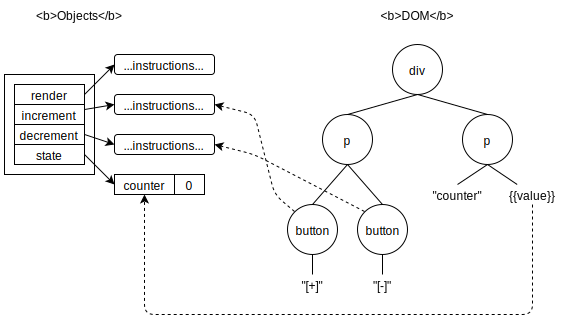
\includegraphics{../../files/interactive-objects-dom.svg}

We must import the dependencies as we did with the other components. As
well as \texttt{React} and \texttt{ReactDOM}, we need to include the
components that we've written. Dependencies stored locally can be
imported by providing the path to the file in which they are defined,
with the \texttt{.js} removed from the file name:

\begin{verbatim}
import React from "react"
import ReactDOM from "react-dom"
import {UpAndDown} from "./UpAndDown"
import {NumberDisplay} from "./NumberDisplay"

// ...script body...
\end{verbatim}

Finally, we can render the application with \texttt{ReactDOM} as before:

\begin{verbatim}
// ...script body...

const mount = document.getElementById("app")
ReactDOM.render(<App/>, mount)
\end{verbatim}

This may seem pretty complicated, and it is, because this example would
be much simpler to write without all this indirection. However, this
strategy is widely used to manage large applications: data and event
handlers are defined in one class, then passed into display components
to be displayed and interacted with.

\subsubsection{Fetching Data}\label{s:interactive-fetching}

Let's use what we've learned to look at how the world might end. NASA
provides a web API to get information about near-approach asteroids. We
will use it to build a small display with:

\begin{itemize}
\tightlist
\item
  a text box for submitting a starting date (get one week by default),
  and
\item
  a list of asteroids in that time period.
\end{itemize}

Here's the first version of our \texttt{App} class:

\begin{verbatim}
import React from "react"
import ReactDOM from "react-dom"
import {AsteroidList} from "./AsteroidList"
import {DateSubmit} from "./DateSubmit"

class App extends React.Component {

  constructor (props) {
    super(props)
    this.state = {
      // ...fill in...
    }
  }

  onNewDate = (text) => {
    // ...fill in...
  }

  render = () => {
    return (
      <div>
        <DateSubmit newValue={this.onNewDate} />
        <AsteroidList asteroids={this.state.asteroids} />
      </div>
    )
  }
}

const mount = document.getElementById("app")
ReactDOM.render(<App/>, mount)
\end{verbatim}

We'll test it by displaying asteroids using fake data; as in our first
example, the display component \texttt{AsteroidList} doesn't modify
data, but just displays it in a table:

\begin{verbatim}
import React from "react"
import ReactDOM from "react-dom"

const AsteroidList = (props) => {
  return (
    <table>
      <tbody>
      <tr><th>Name</th><th>Date</th><th>Diameter (m)</th><th>Approach (km)</th></tr>
      {props.asteroids.map((a) => {
        return (
          <tr key={a.name}>
            <td>{a.name}</td>
            <td>{a.date}</td>
            <td>{a.diameter}</td>
            <td>{a.distance}</td>
          </tr>
        )
      })}
      </tbody>
    </table>
  )
}

export {AsteroidList}
\end{verbatim}

\texttt{React} will complain if we don't provide a unique key to
distinguish elements that we create, since having these keys helps it
keep track of the component-to-DOM relationship, which in turn
\href{https://stackoverflow.com/questions/28329382/understanding-unique-keys-for-array-children-in-react-js}{makes
updates much more efficient}. Since each asteroid's name is supposed to
be unique, we use that name as the key for each table row.

\texttt{AsteroidList} expects data to arrive in
\texttt{props.asteroids}, so let's put some made-up values in
\texttt{App} for now that we can then pass in:

\begin{verbatim}
class App extends React.Component {

  constructor (props) {
    super(props)
    this.state = {
      asteroids: [
        {name: 'a30x1000', date: '2017-03-03', diameter: 30, distance: 1000},
        {name: 'a5x500', date: '2017-05-05', diameter: 5, distance: 500},
        {name: 'a2000x200', date: '2017-02-02', diameter: 2000, distance: 200}
      ]
    }
  }

  // ...other code...
}
\end{verbatim}

Let's also create a placeholder for \texttt{DateSubmit}:

\begin{verbatim}
import React from "react"
import ReactDOM from "react-dom"

const DateSubmit = (props) => {
  return (<p>DateSubmit</p>)
}

export {DateSubmit}
\end{verbatim}

and run it:

Asteroids Application

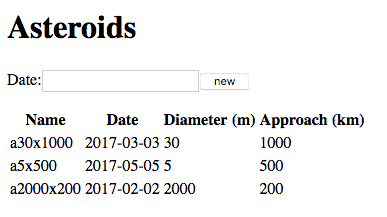
\includegraphics{../../files/interactive-asteroids-screenshot.png}

The next step is to handle date submission. Since we're trying to
instill good practices, we will make a reusable component whose caller
will pass in:

\begin{itemize}
\tightlist
\item
  a text label;
\item
  a variable to update with the current value of a text box;
\item
  a function to call when text box's value changes, and
\item
  another function to call when a button is clicked to submit.
\end{itemize}

\begin{verbatim}
// ...imports as before...

const DateSubmit = ({label, value, onChange, onCommit}) => {
  return (
    <p>
      {label}:
      <input type="text" value={value} onChange={(event) => onChange(event.target.value)} />
      <button onClick={(event) => onCommit(value)}>new</button>
    </p>
  )
}

// ...export as before...
\end{verbatim}

Note the use of destructuring in \texttt{DateSubmit}'s parameter list;
this was introduced \protect\hyperlink{s:pages-citations}{earlier} and
is an easy way to pull values out of the \texttt{props} parameter.

It's important to understand the order of operations in the example
above. \texttt{value=\{value\}} puts a value in the input box to display
each time \texttt{DateSubmit} is called. We re-bind \texttt{onChange}
and \texttt{onClick} to functions on each call as well (remember, JSX
gets translated into function calls). So yes, this whole paragraph is
being re-created every time someone types, but React and the browser
work together to minimize recalculation.

Now let's go back and re-work our application:

\begin{verbatim}
// ...imports as before...

class App extends React.Component {

  constructor (props) {
    super(props)
    this.state = {
      newDate: '',
      asteroids: [...]
    }
  }

  onEditNewDate = (text) => {
    this.setState({newDate: text})
  }

  onSubmitNewDate = (text) => {
    console.log(`new date ${text}`)
    this.setState({newDate: ''})
  }

  render = () => {
    return (
      <div>
        <h1>Asteroids</h1>
        <DateSubmit
          label='Date'
          value={this.state.newDate}
          onChange={this.onEditNewDate}
          onCommit={this.onSubmitNewDate} />
        <AsteroidList asteroids={this.state.asteroids} />
      </div>
    )
  }
}

// ...mount as before...
\end{verbatim}

It's safe to pass \texttt{this.state.newDate} to \texttt{value} because
we're re-drawing each time there's a change; remember, we're passing a
value for display, not a reference to be modified. And note that we are
not doing any kind of validation: the user could type \texttt{abc123} as
a date and we would blithely try to process it.

It's now time to get real data, which we will do using \texttt{fetch}
with a URL. This returns a \protect\hyperlink{s:promises}{promise}, so
we'll handle the result of the fetch in the promise's \texttt{then}
method, and then chain another \texttt{then} method to transform the
data into what we need:

\begin{verbatim}
  onSubmitNewDate = (text) => {
    const url = `https://api.nasa.gov/neo/rest/v1/feed?api_key=DEMO_KEY&start_date=${text}`
    fetch(url).then((response) => {
      return response.json()
    }).then((raw) => {
      const asteroids = this.transform(raw)
      this.setState({
        newDate: '',
        asteroids: asteroids
      })
    })
  }
\end{verbatim}

Line by line, the steps are:

\begin{enumerate}
\tightlist
\item
  Build the URL for the data
\item
  Start to fetch data from that URL
\item
  Give a callback to execute when the data arrives
\item
  Give another callback to use when the data has been converted from
  text to JSON (which we will look at in more detail
  \protect\hyperlink{s:dataman}{soon}).
\item
  Transform that data from its raw form into the objects we need
\item
  Set state
\end{enumerate}

Finally, the method to transform the data NASA gives us is:

\begin{verbatim}
  transform = (raw) => {
    let result = []
    for (let key in raw.near_earth_objects) {
      raw.near_earth_objects[key].forEach((asteroid) => {
        result.push({
          name: asteroid.name,
          date: asteroid.close_approach_data[0].close_approach_date,
          diameter: asteroid.estimated_diameter.meters.estimated_diameter_max,
          distance: asteroid.close_approach_data[0].miss_distance.kilometers
        })
      })
    }
    return result
  }
\end{verbatim}

We built this by looking at the structure of the JSON that NASA returned
and figuring out how to index the fields we need. (Unfortunately, the
top level of \texttt{near\_earth\_objects} is an object with dates as
keys rather than an array, so we have to use \texttt{let...in...} rather
than purely \texttt{map} or \texttt{forEach}.)

\subsubsection{Exercises}\label{s:interactive-exercises}

\paragraph{Reset}\label{reset}

Add a ``reset'' button to the counter application that always sets the
counter's value to zero. Does using it to wipe out every change you've
made to the counter feel like a metaphor for programming in general?

\paragraph{Transform}\label{transform}

Modify all of the examples \emph{after} the introduction of Babel to use
external scripts rather than in-pace scripts.

\paragraph{Exports}\label{exports}

Are the curly braces necessary when exporting from a component file?
What happens if you remove them? Read this
\href{http://2ality.com/2014/09/es6-modules-final.html}{blogpost} and
then consider whether it might have been more appropriate to use default
exports and imports in the examples above.

\paragraph{Validation}\label{validation}

Modify the application so that if the starting date isn't valid when the
button is clicked, the application displays a warning message instead of
fetching data.

\begin{enumerate}
\tightlist
\item
  Add a field called \texttt{validDate} to the state and initialize it
  to \texttt{true}.
\item
  Add an \texttt{ErrorMessage} component that displays a paragraph
  containing either ``date OK'' or ``date invalid'' depending on the
  value of \texttt{validDate}.
\item
  Modify \texttt{onSubmitNewDate} so that it \emph{either} fetches new
  data \emph{or} modifies \texttt{validDate}.
\end{enumerate}

Once you are done, search the Internet for React validation and error
messages and explore other tools you could use to do this.

\textbf{Key Points}

\begin{itemize}
\tightlist
\item
  Define event handlers to specify what actions the browser should take
  when the user interacts with an application.
\item
  The browser passes event objects containing details of events to event
  handlers.
\item
  Use classes to keep state and event handlers together.
\item
  React calls a class's \texttt{render} to display it.
\item
  Separate models (which store data) from views (which display it).
\item
  Use \texttt{fetch} to get data from servers.
\item
  Use destructuring to get individual members from an object in a single
  step.
\item
  Modern JavaScript uses promises to manage asynchronous activities.
\end{itemize}

\hypertarget{s:dataman}{\subsection{Managing Data}\label{s:dataman}}

\textbf{Questions}

\begin{itemize}
\tightlist
\item
  What formats are commonly used for small scientific datasets?
\item
  What are some of the strengths and weaknesses of those formats?
\item
  How can I parse CSV data?
\item
  How should I select a subset of data for testing purposes?
\end{itemize}

There's not much point creating interactive web pages if they don't have
something to interact with. To provide that, we need something to store
data and something to serve it. We could build one program to do both,
but experience teaches that it's better to create one for each so that
they are easier to understand, test, and maintain. After tossing a coin,
we decide to start with the data store; the
\protect\hyperlink{s:server}{next lesson} will look at how to build a
server.

\subsubsection{Data Formats}\label{s:data-formats}

The most widely used text format for tabular data is undoubtedly
\protect\hyperlink{g:csv}{comma-separated values} or CSV. Each row of
the table is a line in the file; the values within each row---i.e., the
columns---are separated by commas. Numbers appear as themselves; strings
may or may not be wrapped in quotation marks, unless they contain commas
themselves, in which case they definitely are:

\begin{verbatim}
"maroon",128,0,0
"olive",128,128,0
"aqua",0,255,255
"fuchsia",255,0,255
\end{verbatim}

The first line of a CSV file is often a
\protect\hyperlink{g:header-row}{header row} that defines the names of
the columns. For example, the small table shown above would better be
represented as:

\begin{verbatim}
"name","red","green","blue"
"maroon",128,0,0
"olive",128,128,0
"aqua",0,255,255
"fuchsia",255,0,255
\end{verbatim}

Tragically, CSV doesn't require the first row to be a header, and CSV
files usually don't specify units or data types. We can guess that the
values in the table above are integers, but it's all too common to have
a CSV file whose columns are labelled ``height'' and ``weight'' without
any indication of whether the heights are in feet or meters or the
weights in pounds or kilograms.

CSV is good for tabular data, but a lot of data doesn't neatly fit into
rows and columns. A format for hierarchical data that is popular with
many programmers is \protect\hyperlink{g:json}{JSON}, which stands for
JavaScript Object Notation. It supports a subset of the syntax for
values, arrays, and objects in JavaScript, so that (for example) we can
store configuration values for a program like this:

\begin{verbatim}
{
  "name" : "DataExplorer",
  "version" : "1.2.1",
  "preferences" : {
    "colorscheme" : "dark",
    "autofill" : true
  },
  "last_opened" : [
    "raw/biotic.dat",
    "raw/genomic.dat",
    "cooked/inferred.dat"
  ]
}
\end{verbatim}

JSON can be used for tabular data as well. The whole table is an array,
and each record is an object with name-value pairs:

\begin{verbatim}
[
  {"name": "maroon", "red": 128, "green": 0, "blue": 0},
  {"name": "olive", "red": 128, "green": 128, "blue": 0},
  {"name": "aqua", "red": 0, "green": 255, "blue": 255},
  {"name": "fuchsia", "red": 255, "green": 0, "blue": 255}
]
\end{verbatim}

Repeating field names like this is wasteful compared to listing them
once at the top of a table, but it does mean that the fields within rows
can be accessed directly using expressions like
\texttt{colors{[}1{]}.red}.

\subsubsection{Slicing Data}\label{s:data-slicing}

The data we will use as an example is available in a variety of formats
from
\url{https://figshare.com/articles/Portal_Project_Teaching_Database/1314459}.
We will focus on \texttt{surveys.csv}, which has over 35,500 records.
That's a lot to look at, so we will create a 10-record slice for
testing.

Although it would be easy to take the first ten, or the last, there's a
good chance that neither would be representative of the data as a whole.
Instead, we will write a little script that selects N records at random.
Since it doesn't need to be efficient, we will do something simple:

\begin{verbatim}
const fs = require('fs')

const [inputFile, numLines, outputFile] = process.argv.splice(2)
const lines = fs.readFileSync(inputFile, 'utf-8')
    .split('\n')
header = lines[0]
const sample = lines.slice(1)
    .map(line => [Math.random(), line])
    .sort((left, right) => { return left[0] - right[0] })
    .slice(0, parseInt(numLines))
    .map(pair => pair[1])
fs.writeFileSync(outputFile, header + '\n' + sample.join('\n'))
\end{verbatim}

We run this on the command line:

\begin{verbatim}
node select-random.js ../surveys.csv 10 slice.csv
\end{verbatim}

and get this:

\begin{verbatim}
record_id,month,day,year,plot_id,species_id,sex,hindfoot_length,weight
18501,3,14,1991,13,OT,M,21,28
2283,1,15,1980,11,OL,M,21,23
19941,5,2,1992,1,PP,M,22,13
27413,12,29,1997,5,,,,
16002,5,9,1989,19,SC,,,
28813,11,21,1998,12,DO,M,35,56
9338,7,4,1984,11,DO,F,35,57
28336,8,22,1998,7,PB,M,26,23
25323,3,16,1997,9,DM,F,33,26
6785,10,23,1982,5,DM,F,37,45
\end{verbatim}

Running it again will probably generate a different data slice, since
we're not specifying a random number generation seed. We are bad people,
and will fix this in the exercises.

\subsubsection{Data Manager}\label{s:data-manager}

Rather arbitrarily, we decide that our data manager will be able to
answer two questions:

\begin{enumerate}
\tightlist
\item
  How many records do we have and what range of years do they cover?
  This is the kind of opening question that many client programs will
  ask.
\item
  What are the minimum, average, and maximum values for weight and
  hindfoot length by year for a given range of years? This would be very
  specific to a particular kind of client program; a good service would
  either provide many such specialized queries or provide a way to apply
  common \protect\hyperlink{g:aggregation-function}{aggregation
  functions} to particular columns.
\end{enumerate}

We will use \href{https://www.papaparse.com/}{PapaParse} to parse our
CSV, so our first step is to install it:

\begin{verbatim}
npm install papaparse
\end{verbatim}

After loading the library and reading our test data file a couple of
times, we break down and read the documentation, then come up with this
as the first version of our data manager:

\begin{verbatim}
const fs = require('fs')
const papa = require('papaparse')

class DataManager {

  constructor (filename) {
    const raw = fs.readFileSync(filename, 'utf-8')
    const options = {header: true, dynamicTyping: true}
    this.data = papa.parse(raw, options).data
  }
}

module.exports = DataManager
\end{verbatim}

What our hubris made us miss in our first couple of attempts was that
the \texttt{options} object controls how the parser behaves. Here, we
tell it to interpret the first row as a header (which sets column names)
and to convert things that look like numbers to numbers (the
\texttt{dynamicTyping} option). The output of \texttt{papa.parse} looks
like this:

\begin{verbatim}
{ data:
   [ { record_id: 18501,
       month: 3,
       day: 14,
       year: 1991,
       plot_id: 13,
       species_id: 'OT',
       sex: 'M',
       hindfoot_length: 21,
       weight: 28 },

     ...eight more records...

     { record_id: 6785,
       month: 10,
       day: 23,
       year: 1982,
       plot_id: 5,
       species_id: 'DM',
       sex: 'F',
       hindfoot_length: 37,
       weight: 45 } ],
  errors: [],
  meta:
   { delimiter: ',',
     linebreak: '\n',
     aborted: false,
     truncated: false,
     cursor: 350,
     fields:
      [ 'record_id',
        'month',
        'day',
        'year',
        'plot_id',
        'species_id',
        'sex',
        'hindfoot_length',
        'weight' ] } }
\end{verbatim}

so using \texttt{papa.parse(raw,\ options).data} gets the data we want
as JSON. Let's write a method to get some overall statistics:

\begin{verbatim}
  getSurveyStats () {
    return {
      minYear : this._get('year', Math.min),
      maxYear : this._get('year', Math.max),
      count : this.data.length
    }
  }

  _get(field, func) {
    return func(...this.data.map(rec => rec[field]))
  }
\end{verbatim}

Functions like \texttt{Math.min} and \texttt{Math.max} take any number
of scalar values as arguments, but do not directly process arrays.
However, the notation \texttt{func(...array)} means ``pass all the
values in the array as separate arguments'', which saves us from writing
our own minimum and maximum functions. Thus,
\texttt{func(...this.data.map(rec\ =\textgreater{}\ rec{[}field{]}))}
means ``select the specified field from each record in
\texttt{this.data} to create an array of fields, then pass all of those
values as arguments to \texttt{func}. We include an underscore to the
start of the name of \texttt{\_get} to indicate that we intend it to be
used only inside \texttt{DataManager} and not to be called elsewhere.

Adding the method to get weight and hindfoot length for a range of years
is comparatively straightforward. First, we write a function to
calculate the average of one or more arguments:

\begin{verbatim}
const _average = (...values) => {
  let sum = 0
  for (let v of values) {
    sum += v
  }
  return sum / values.length
}
\end{verbatim}

It would be more natural for \texttt{\_average} to take an array rather
than a variable number of arguments, but we want to be able to use it in
the same way that we use \texttt{Math.min} and \texttt{Math.max}, so we
have to conform to their signature.

After some thought we realize that it's possible for \texttt{subset} to
be empty - that is, it's possible that there are years that have no data
in our data set. We should filter these out, to prevent unnecessary
effort being made to render summary statistics with \texttt{NaN} values.
Remembering that \protect\hyperlink{s:basics}{empty arrays are not falsy
in JavaScript}, we decide to test that the \texttt{subset} returned by
filtering for each year contains at least one entry.

The last thing that we need to ensure is that each data object has a
unique key, which will make it much easier for React to efficiently
update the display of the data when we are ready to render it.

The method to get the values for a range of years is now:

\begin{verbatim}
  getSurveyRange (minYear, maxYear) {
    return Array(1 + maxYear - minYear)
      .fill(0)
      .map((v, i) => minYear + i)
      .map(year => {
    const subset = this.data.filter(r => r.year === year)
      if (subset.length) {
        return {
          key  : toString(year),
          year : year,
          min_hindfoot_length : this._get(subset, 'hindfoot_length', Math.min),
          ave_hindfoot_length : this._get(subset, 'hindfoot_length', _average),
          max_hindfoot_length : this._get(subset, 'hindfoot_length', Math.max),
          min_weight : this._get(subset, 'weight', Math.min),
          ave_weight : this._get(subset, 'weight', _average),
          max_weight : this._get(subset, 'weight', Math.max)
        }
      }
    })
  }
\end{verbatim}

\subsubsection{Exercises}\label{s:data-exercises}

\paragraph{Tracing Data}\label{tracing-data}

Trace the execution of the utility program that creates a small sample
of the original data, explaining what is passed into each of the chained
methods calls.

\paragraph{Unrandom}\label{unrandom}

Programs that rely on random numbers are impossible to test because
there's (deliberately) no way to predict their output. Luckily, computer
programs don't actually use random numbers: they use
\protect\hyperlink{g:pseudo-random-number}{pseudo-random numbers} that
are generated in a repeatable but unpredictable way. Given the same
initial \protect\hyperlink{g:seed}{seed}, a pseudo-random number
generator will always produce the same sequence of values.

There is no way to set a seed for \texttt{Math.random} out of the box,
but the \href{https://www.npmjs.com/package/seedrandom}{seedrandom}
package provides an add-on function for this purpose. Install the
package and modify the slice selection utility so that it takes a word
or phrase as a command-line argument and uses it to seed the random
number generator.

\paragraph{One Record Per Year}\label{one-record-per-year}

Another way to slice the data for testing purposes is to select one
record from each year. Write a small command-line JavaScript program
that:

\begin{enumerate}
\tightlist
\item
  Reads all the data from the CSV.
\item
  Keeps the first record it finds for each year.
\item
  Prints these records formatted as SQL \texttt{insert} statements.
\end{enumerate}

\paragraph{Error Handling}\label{error-handling}

Modify \texttt{DataManager}'s constructor so that it checks for errors.

\paragraph{Generalization}\label{generalization}

Modify \texttt{getSurveyRange} so that it can be called like this:

\begin{verbatim}
getSurveyRange(minYear, maxYear, 'hindfoot_length', 'weight')
\end{verbatim}

i.e., so that the names of the fields whose minimum, average, and
maximum values are wanted can be passed as strings, and the method will
automatically create the right names and values in its result.

\textbf{Key Points}

\begin{itemize}
\tightlist
\item
  Small tabular datasets are commonly stored as Comma-Separated Values
  (CSV).
\item
  CSV can only represent regular data, and CSV files usually don't
  include units.
\item
  Nested data is commonly stored using JavaScript Object Notation
  (JSON).
\item
  JSON representations of tabular data often include redundant (and
  therefore possibly inconsistent) specifications of column names.
\item
  PapaParse is a robust CSV parsing library that produces JSON output.
\end{itemize}

\hypertarget{s:server}{\subsection{Creating a Server}\label{s:server}}

\textbf{Questions}

\begin{itemize}
\tightlist
\item
  How do browsers and servers communicate?
\item
  What tools can I use to create a data server in JavaScript?
\item
  How can I tell a server to handle different URLs differently?
\item
  How can I serve files from disk?
\item
  How does a server specify the type of data it's sending?
\item
  How can I add new abilities to a server without rewriting it?
\end{itemize}

Now that we have \protect\hyperlink{s:dataman}{a data manager}, the next
step is to create a server to share our data with the world, which we
will build using a library called
\href{https://expressjs.org/}{Express}. Before we start writing code,
though, we need to understand how computers talk to each other.

\subsubsection{HTTP}\label{s:server-http}

Almost everything on the web communicates via
\protect\hyperlink{g:http}{HTTP}, which stands for HyperText Transfer
Protocol. The core of HTTP is a
\protect\hyperlink{g:http-request}{request}/\protect\hyperlink{g:http-response}{response}
cycle that specifies the kinds of requests applications can make of
servers, how they exchange data, and so on. The diagram below shows this
cycle in action for a page that includes one image:

\begin{enumerate}
\tightlist
\item
  The client (a browser or some other program) makes a connection to a
  server.
\item
  It then sends a blob of text specifying what it's asking for.
\item
  The server replies with a blob of text and the HTML.
\item
  The connection is closed.
\item
  The client parses the text and realizes it needs an image.
\item
  It sends another blob of text to the server asking for that image.
\item
  The server replies with a blob of text and the contents of the image
  file.
\item
  The connection is closed.
\end{enumerate}

HTTP Request/Response Cycle

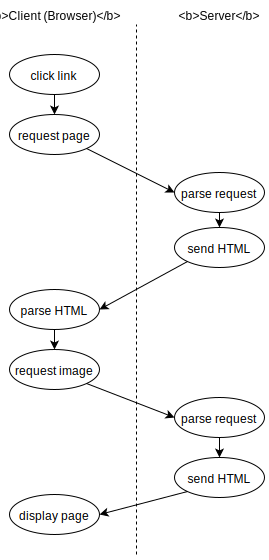
\includegraphics{../../files/server-cycle.svg}

This cycle might be repeated many times to display a single web page,
since a separate request has to be made for every image, every CSS or
JavaScript file, and so on. In practice, a lot of behind-the-scenes
engineering is done to keep connections alive as long as they're needed,
and to \protect\hyperlink{g:cache}{cache} items that are likely to be
re-used.

An HTTP request is just a block of text with two important parts:

\begin{itemize}
\tightlist
\item
  The \protect\hyperlink{g:http-method}{method} is almost always either
  \texttt{GET} (to get data) or \texttt{POST} (to submit data).
\item
  The \protect\hyperlink{g:url}{URL} is typically a path to a file, but
  as we'll see below, it's completely up to the server to interpret it.
\end{itemize}

The request can also contain \protect\hyperlink{g:http-header}{headers},
which are key-value pairs with more information about what the client
wants. Some examples include:

\begin{itemize}
\tightlist
\item
  \texttt{"Accept:\ text/html"} to specify that the client wants HTML
\item
  \texttt{"Accept-Language:\ fr,\ en"} to specify that the client
  prefers French, but will accept English
\item
  \texttt{"If-Modified-Since:\ 16-May-2018"} to tell the server that the
  client is only interested in recent data
\end{itemize}

(Unlike a dictionary, a key may appear any number of times, which allows
a request to do things like specify that it's willing to accept several
types of content. The \protect\hyperlink{g:http-body}{body} of the
request is any extra data associated with it, such as files that are
being uploaded. If a body is present, the request must contain the
\texttt{Content-Length} header so that the server knows how much data to
read.

Structure of an HTTP Request


\includegraphics{../../files/server-request.svg}

The headers and body in an HTTP response have the same form, and mean
the same thing. Crucially, the response also includes a status code to
indicate what happened: 200 for OK, 404 for ``page not found'', and so
on. Some of the more common are:

\begin{longtable}[]{@{}lll@{}}
\toprule
Code & Name & Meaning\tabularnewline
\midrule
\endhead
100 & Continue & The client should continue sending data\tabularnewline
200 & OK & The request has succeeded\tabularnewline
204 & No Content & The server completed the request but doesn't need to
return any data\tabularnewline
301 & Moved Permanently & The requested resource has moved to a new
permanent location\tabularnewline
307 & Temporary Redirect & The requested resource is temporarily at a
different location\tabularnewline
400 & Bad Request & The request is badly formatted\tabularnewline
401 & Unauthorized & The request requires authentication\tabularnewline
404 & Not Found & The requested resource could not be
found\tabularnewline
408 & Timeout & The server gave up waiting for the client\tabularnewline
418 & I'm a Teapot & Originally an April Fool's joke, now used to
identify devices\tabularnewline
500 & Internal Server Error & An error occurred in the server while
trying to handle the request\tabularnewline
601 & Connection Timed Out & The server did not respond before the
connection timed out\tabularnewline
\bottomrule
\end{longtable}

One final thing we need to understand is the structure and
interpretation of URLs. This one:

\begin{verbatim}
http://example.org:1234/some/path?value=deferred&limit=200
\end{verbatim}

has five parts:

\begin{itemize}
\tightlist
\item
  The protocol \texttt{http}, which specifies what rules are going to be
  used to exchange data.
\item
  The \protect\hyperlink{g:hostname}{hostname} \texttt{example.org},
  which tells the client where to find the server. If we are running a
  server on our own computer for testing, we can use the name
  \texttt{localhost} to connect to it. (Computers rely on a service
  called \protect\hyperlink{g:dns}{DNS} to find the machines associated
  with human-readable hostnames, but its operation is out of scope for
  this tutorial.)
\item
  The \protect\hyperlink{g:port}{port} \texttt{1234}, which tells the
  client where to call the service it wants. (If a host is like an
  office building, a port is like a phone number in that building. The
  fact that we think of phone numbers as having physical locations says
  something about our age\ldots{})
\item
  The path \texttt{/some/path} tells the server what the client wants.
\item
  The \protect\hyperlink{g:query-parameter}{query parameters}
  \texttt{value=deferred} and \texttt{limit=200}. These come after a
  question mark and are separated by ampersands, and are used to provide
  extra information.
\end{itemize}

It used to be common for paths to identify actual files on the server,
but the server can interpret the path however it wants. In particular,
when we are writing a data service, the segments of the path can
identify what data we are asking for. Alternatively, it's common to
think of the path as identifying a function on the server that we want
to call, and to think of the query parameters as the arguments to that
function. We'll return to these ideas after we've seen how a simple
server works.

\subsubsection{Hello, Express}\label{s:server-express}

A Node-based library called Express handles most of the details of HTTP
for us. When we build a server using Express, we provide callback
functions that take three parameters:

\begin{itemize}
\tightlist
\item
  the original request,
\item
  the response we're building up, and
\item
  what to do next (which we'll ignore for now).
\end{itemize}

We also provide a pattern with each function that specifies what URLs it
is to match. Here is a simple example:

\begin{verbatim}
const express = require('express')

const PORT = 3418

// Main server object.
const app = express()

// Return a static page.
app.get('/', (req, res, next) => {
  res.status(200).send('<html><body><h1>Asteroids</h1></body></html>')
})

app.listen(PORT, () => { console.log('listening...') })
\end{verbatim}

The first line of code loads the Express library. The next defines the
port we will listen on, and then the third creates the object that will
do most of the work.

Further down, the call to \texttt{app.get} tells that object to handle
any \texttt{GET} request for `/' by sending a reply whose status is 200
(OK) and whose body is an HTML page containing only an \texttt{h1}
heading. There is no actual HTML file on disk, and in fact no way for
the browser to know if there was one or not: the server can send
whatever it wants in response to whatever requests it wants to handle.

Note that \texttt{app.get} doesn't actually get anything right away.
Instead, it registers a callback with Express that says, ``When you see
this URL, call this function to handle it.'' As we'll see below, we can
register as many path/callback pairs as we want to handle different
things.

Finally, the last line of this script tells our application to listen on
the specified port, while the callback tells it to print a message as it
starts running. When we run this, we see:

\begin{verbatim}
node static-page.js
\end{verbatim}

\begin{verbatim}
listening...
\end{verbatim}

Our little server is now waiting for something to ask it for something.
If we go to our browser and request \texttt{http://localhost:3418/}, we
get a page with a large title \texttt{Asteroids} on it. Our server has
worked, and we can now stop it by typing Ctrl-C in the shell.

\subsubsection{Handling Multiple Paths}\label{s:server-paths}

Let's extend our server to do different things when given different
paths, and to handle the case where the request path is not known:

\begin{verbatim}
const express = require('express')

const PORT = 3418

// Main server object.
const app = express()

// Root page.
app.get('/', (req, res, next) => {
  res.status(200).send('<html><body><h1>Home</h1></body></html>')
})

// Alternative page.
app.get('/asteroids', (req, res, next) => {
  res.status(200).send('<html><body><h1>Asteroids</h1></body></html>')
})

// Nothing else worked.
app.use((req, res, next) => {
  res.status(404).send(`<html><body><h1>ERROR</h1><p>URL "${req.url}" not found</p></body></html>`)
})

app.listen(PORT, () => { console.log('listening...') })
\end{verbatim}

The first few lines are the same as before. We then specify handlers for
the paths \texttt{/} and \texttt{/asteroids}, each of which sends a
different chunk of HTML.

The call to \texttt{app.use} specifies a default handler: if none of the
\texttt{app.get} handlers above it took care of the request, this
callback function will send a ``page not found'' code \emph{and} a page
containing an error message. Some sites skip the first part and only
return error messages in pages for people to read, but this is sinful:
making the code explicit makes it a lot easier to write programs to
scrape data.

As before, we can run our server from the command line and then go to
various URLs to test it. \texttt{http://localhost:3418/} produces a page
with the title ``Home'', \texttt{http://localhost:3418/asteroids}
produces one with the title ``Asteroids'', and
\texttt{http://localhost:3418/test} produces an error page.

\subsubsection{Serving Files from Disk}\label{s:server-files}

It's common to generate HTML in memory when building data services, but
it's also common for the server to return files. To do this, we will
provide our server with the path to the directory it's allowed to read
pages from, and then run it with
\texttt{node\ server-name.js\ path/to/directory}. We have to tell the
server whence it's allowed to read files because we definitely do
\emph{not} want it to be able to send everything on our computer to
whoever asks for it. (For example, a request for the
\texttt{/etc/passwd} password file on a Linux server should probably be
refused.)

Here's our updated server:

\begin{verbatim}
const express = require('express')
const path = require('path')
const fs = require('fs')

const PORT = 3418
const root = process.argv[2]

// Main server object.
const app = express()

// Handle all requests.
app.use((req, res, next) => {
  const actual = path.join(root, req.url)
  const data = fs.readFileSync(actual, 'utf-8')
  res.status(200).send(data)
})

app.listen(PORT, () => { console.log('listening...') })
\end{verbatim}

The steps in handling a request are:

\begin{enumerate}
\tightlist
\item
  The URL requested by the client is given to us in \texttt{req.url}.
\item
  We use \texttt{path.join} to combine that with the path to the root
  directory, which we got from a command-line argument when the server
  was run.
\item
  We try to read that file using \texttt{readFileSync}, which blocks the
  server until the file is read. We will see later how to do this I/O
  asynchronously so that our server is more responsive.
\item
  Once the file has been read, we return it with a status code of 200.
\end{enumerate}

If a sub-directory called \texttt{web-dir} holds a file called
\texttt{title.html}, and we run the server as:

\begin{verbatim}
node serve-pages.js ./web-dir
\end{verbatim}

we can then ask for \texttt{http://localhost:3418/title.html} and get
the content of \texttt{web-dir/title.html}. Notice that the directory
\texttt{./web-dir} doesn't appear in the URL: our server interprets all
paths as if the directory we've given it is the root of the filesystem.

If we ask for a page that doesn't exist, such as
\texttt{http://localhost:3418/missing.html}, we get this:

\begin{verbatim}
Error: ENOENT: no such file or directory, open 'web-dir/missing.html'
    at Object.openSync (fs.js:434:3)
    at Object.readFileSync (fs.js:339:35)
    ... etc. ...
\end{verbatim}

We will see in the exercises how to add proper error handling to our
server.

\begin{quote}
\textbf{Favorites and Icons}

If we use a browser to request a page such as \texttt{title.html}, the
browser may actually make two requests: one for the page, and one for a
file called \texttt{favicon.ico}. Browsers do this automatically, then
display that file in tabs, bookmark lists, and so on. Despite its
\texttt{.ico} suffix, the file is (usually) a small PNG-formatted image,
and must be placed in the root directory of the website.
\end{quote}

\subsubsection{Content Types}\label{s:server-content-types}

So far we have only served HTML, but the server can send any type of
data, including images and other binary files. For example, let's serve
some JSON data:

\begin{verbatim}
// ...as before...

app.use((req, res, next) => {
  const actual = path.join(root, req.url)

  if (actual.endsWith('.json')) {
    const data = fs.readFileSync(actual, 'utf-8')
    const json = JSON.parse(data)
    res.setHeader('Content-Type', 'application/json')
    res.status(200).send(json)
  }

  else {
    const data = fs.readFileSync(actual, 'utf-8')
    res.status(200).send(data)
  }
})
\end{verbatim}

What's different here is that when the requested path ends with
\texttt{.json} we explicitly set the \texttt{Content-Type} header to
\texttt{application/json} to tell the client how to interpret the bytes
we're sending back. If we run this server with \texttt{web-dir} as the
directory to serve from and ask for
\texttt{http://localhost:3418/data.json}, a modern browser will provide
a folding display of the data rather than displaying the raw text.

\subsubsection{Exercises}\label{s:server-exercises}

\paragraph{Report Missing Files}\label{report-missing-files}

Modify the version of the server that returns files from disk to report
a 404 error if a file cannot be found. What should it return if the file
exists but cannot be read (e.g., if the server does not have
permissions)?

\paragraph{Serving Images}\label{serving-images}

Modify the version of the server that returns files from disk so that if
the file it is asked for has a name ending in \texttt{.png} or
\texttt{.jpg}, it is returned with the right \texttt{Content-Type}
header.

\paragraph{Delayed Replies}\label{delayed-replies}

Our file server uses \texttt{fs.readFileSync} to read files, which means
that it stops each time a file is requested rather than handling other
queries while waiting for the file to be read. Modify the callback given
to \texttt{app.use} so that it uses \texttt{fs.readFile} with a callback
instead.

\paragraph{Using Query Parameters}\label{using-query-parameters}

URLs can contain query parameters in the form
\texttt{http://site.edu?first=1\&second=b}. Read the online
documentation for \href{https://expressjs.org/}{Express} to find out how
to access them in a server, and then write a server to do simple
arithmetic: the URL \texttt{http://localhost:3654/add?left=1\&right=2}
should return \texttt{3}, while the URL
\texttt{http://localhost:3654/subtract?left=1\&right=2} should return
\texttt{-1}.

\textbf{Key Points}

\begin{itemize}
\tightlist
\item
  An HTTP request or response consists of a plain-text header and an
  optional body.
\item
  HTTP is a stateless protocol.
\item
  Express provides a simple path-based JavaScript server.
\item
  Write callback functions to handle requests matching specified paths.
\item
  Provide a default handler for unrecognized requests.
\item
  Use \texttt{Content-Type} to specify the type of data being returned.
\item
  Use dynamic loading to support plugin extensions.
\end{itemize}

\hypertarget{s:testing}{\subsection{Testing}\label{s:testing}}

\textbf{Questions}

\begin{itemize}
\tightlist
\item
  How should software components be tested?
\item
  What tools can I use to test JavaScript programs?
\item
  How can I make software easier to test?
\item
  How can testing code drive a web server?
\item
  How can tests check the content of HTML pages?
\item
  How is HTML represented in a JavaScript program?
\end{itemize}

We are bad people, because we have been writing code without testing it.
In this lesson we will redeem ourselves (partially) by correcting that
(also partially).

JavaScript uses the same pattern for
\protect\hyperlink{g:unit-test}{unit testing} as most other modern
languages. Each test is written as a function, and each of those
functions tests one particular aspect of the code. A standalone program
called a \protect\hyperlink{g:test-runner}{test runner} finds test
functions, runs them, and reports the results. Any setup code that needs
to be run before each test to create a
\protect\hyperlink{g:fixture}{fixture} is put in a function of its own.
Similarly (but less frequently), if some teardown needs to be done
\emph{after} each test, we put those operations in a function as well.

Each unit test can have one of three results:

\begin{itemize}
\tightlist
\item
  pass: everything worked
\item
  fail: the system being tested didn't do what was expected
\item
  error: something went wrong with the test itself
\end{itemize}

We can combine tests into \protect\hyperlink{g:test-suite}{test suites}
(and test suites into larger suites, and so on) so that we can more
easily run related sets of tests. This makes testing during development
faster, which in turn makes it more likely that we'll actually do it.

Finally, we write the tests themselves using
\protect\hyperlink{g:assertion}{assertions}: statements that check
whether or not some condition holds and generate an error if it doesn't.
Node provides an \texttt{assert} library with some useful functions for
asserting various things; we'll explore this as we go along.

\subsubsection{Introducing Mocha}\label{s:testing-mocha}

JavaScript has almost as many testing libraries as it has front-end
frameworks. We will use one called \href{https://mochajs.org/}{Mocha}
that is popular and well documented. Unlike the libraries we have seen
before, we don't import anything to use it; instead, \emph{it} imports
\emph{our} code and calls our functions.

When we're writing tests for Mocha to run, we use a function called
\texttt{describe} to create a group of tests and another function called
\texttt{it} for each test in that group:

\begin{verbatim}
describe('first test', () => {
  it('should run without errors', (done) => {
    done()
  })
})
\end{verbatim}

As this example shows, \texttt{describe}'s arguments are an explanatory
string and a callback function. That callback makes calls to
\texttt{it}, which takes:

\begin{itemize}
\tightlist
\item
  another explanatory string describing how the system should behave,
  and
\item
  a callback that receives a function (called \texttt{done} by
  convention).
\end{itemize}

(The name \texttt{it} was chosen so that when we read tests aloud, it
sounds like we're saying, ``It should do this or that.'') At the end of
each test we call \texttt{done} to signal that it has finished. We have
to do this because callbacks run out of order, so Mocha needs to know
when each one completes.

We can run our tests from the shell by invoking \texttt{mocha} and
giving it the path to the file that contains the tests:

\begin{verbatim}
./node_modules/.bin/mocha path/to/test.js
\end{verbatim}

\begin{verbatim}
  first test
    + should run without errors


  1 passing (12ms)
\end{verbatim}

As with bundling, we normally put the \texttt{mocha} command in
\texttt{package.json} so that \texttt{./node\_modules/.bin} is
automatically included in the path. After we add this:

\begin{verbatim}
{
  ...
  "scripts": {
    ...
    "test": "mocha",
    ...
  }
}
\end{verbatim}

to \texttt{package.json}, our command becomes:

\begin{verbatim}
npm test -- path/to/test.js
\end{verbatim}

(Again, everything after \texttt{-\/-} is passed to the script itself.)

\subsubsection{Refactoring}\label{s:testing-refactoring}

The next step is to create testable software. In the case of our server,
we have to:

\begin{itemize}
\tightlist
\item
  move the code that listens on a port into one file, and
\item
  have that import a file that contains the code to do everything else.
\end{itemize}

Once we have done this, we can run the server code in other contexts.
Here's the file \texttt{standalone.js} that actually launches a server:

\begin{verbatim}
const server = require('./server')
const PORT = 3418
server.listen(PORT, () => { console.log(`listening on port ${PORT}...`) })
\end{verbatim}

And here is the application code we've extracted into \texttt{server.js}
so that we can test it:

\begin{verbatim}
const express = require('express')

// Main server object.
let app = express()

// Root page.
app.get('/', (req, res, next) => {
  res.status(200).send('<html><body><h1>Home</h1></body></html>')
})

// ...as before...

module.exports = app
\end{verbatim}

Before going any further, we can check that we haven't broken anything
by running:

\begin{verbatim}
node standalone.js
\end{verbatim}

\subsubsection{Testing the Server}\label{s:testing-server}

All right: now that we have extracted the code that's specific to our
server, how do we test it? The answer is yet another library called
\href{https://github.com/visionmedia/supertest}{supertest} that sends
fake HTTP requests to an Express server that has been split in the way
we just split ours and lets us interact with that server's replies.
Here's a test of a simple request that uses Mocha to manage the test,
and supertest's \texttt{request} function to send something to the
server and check the result:

\begin{verbatim}
const assert = require('assert')
const request = require('supertest')
const server = require('./server')

describe('server', () => {

  it('should return HTML with expected title', (done) => {
    request(server)
      .get('/')
      .expect(200)
      .expect('Content-Type', /html/)
      .end((err, res) => {
        assert(res.text.includes('Home'), 'Has expected title')
        done()
      })
  })
})
\end{verbatim}

Going through this line by line:

\begin{enumerate}
\tightlist
\item
  \texttt{request(server)} starts building up a request to send.
\item
  \texttt{.get(\textquotesingle{}/\textquotesingle{})} specifies the
  path in the URL we are sending.
\item
  \texttt{.expect(200)} checks that the return code is 200 (OK).
\item
  \texttt{.expect(\textquotesingle{}Content-Type\textquotesingle{},\ /html/)}
  checks the content type in the returned value against a regular
  expression (discussed briefly at the end of this section).
\item
  \texttt{.end} is called when the whole response has been received,
  i.e., when we can start looking at the content of the page or data
  that the server has sent.
\item
  Inside the callback to \texttt{end}, \texttt{res} is the result data.
  We make sure that its text (i.e., \texttt{res.text}) includes the word
  ``Home''. We really should check \texttt{err} here to make sure
  everything worked properly, but we're not quite that virtuous.
\item
  Finally, we call \texttt{done()} to signal the end of the test. Again,
  we have to do this because there's no way Mocha can know when the
  enclosing \texttt{.end(...)} will be called
\end{enumerate}

Let's run our code:

\begin{verbatim}
  server
    + should return HTML with expected title (48ms)


  1 passing (58ms)
\end{verbatim}

Excellent: let's add some more tests.

\begin{verbatim}
describe('server', () => {

  it('should return HTML with expected title', (done) => {
    // ...as before...
  })

  it('should return asteroids page as HTML with expected title', (done) => {
    request(server)
      .get('/asteroids')
      .expect(200)
      .expect('Content-Type', /html/)
      .end((err, res) => {
        assert(res.text.includes('Asteroids'), 'Has expected title')
        done()
      })
  })

  it('should 404 for other pages', (done) => {
    request(server)
      .expect(404)
      .get('/other')
      .end((err, res) => {
        assert(res.text.includes('ERROR'), 'Has expected error message')
        done()
      })
  })
})
\end{verbatim}

\begin{verbatim}
  server
    + should return HTML with expected title (42ms)
    + should return asteroids page as HTML with expected title
    + should 404 for other pages


  3 passing (62ms)
\end{verbatim}

Notice that we check to make sure that the server sends a 404 when we
ask for something that doesn't exist. Making sure the system fails
gracefully is just as important as making sure that it provides data
when asked to.

\subsubsection{Checking the HTML}\label{s:testing-html}

It's increasingly common for servers to return data that is then
rendered by the client, but some servers still generate HTML. Do
\emph{not} try to check this with substrings or regular expressions: the
exceptions have exceptions, and
\href{https://stackoverflow.com/a/1732454}{that way lies madness}.
Instead, we should parse the HTML to create a structure in memory and
check that; if parsing fails because the HTML is badly formatted, that's
worth knowing too. The structure in question is our new friend the DOM,
and to get it, we will use (yet another) library called
\href{https://cheerio.js.org/}{cheerio}. \texttt{cheerio.load} turns
HTML text into a DOM tree; the resulting object can be used like a
function, and we can use the same selectors we met previously to find
things in it. Here's our test:

\begin{verbatim}
const assert = require('assert')
const request = require('supertest')
const cheerio = require('cheerio')
const server = require('./server')

describe('server', () => {
  it('should have the correct headings', (done) => {
    request(server)
      .get('/')
      .expect('Content-Type', /html/)
      .expect(200)
      .end((err, res) => {
        const tree = cheerio.load(res.text)
        assert.equal(tree('h1').length, 1, 'Correct number of headings')
        assert.equal(tree('h1').text(), 'Home', 'Correct heading text')
        done()
      })
  })
})
\end{verbatim}

\begin{verbatim}
  server
    + should have the correct headings (67ms)


  1 passing (77ms)
\end{verbatim}

This gets the page as before, parses it, then looks for \texttt{h1}
elements and checks the text of the first one. (Note that this
\emph{doesn't} check if the title is
\texttt{\textless{}em\textgreater{}H\textless{}/em\textgreater{}ome}
because \texttt{.text()} concatenates all the text of the children.) We
won't explore this approach further because we're going to serve data
for rendering rather than generating HTML and sending that, but if
you're doing any web scraping at all, libraries like \texttt{cheerio}
are there to help.

\subsubsection{Exercises}\label{s:testing-exercises}

\paragraph{Not Done}\label{not-done}

What happens if we forget to call \texttt{done()} in a test?

\paragraph{Adding Tests}\label{adding-tests}

\begin{enumerate}
\tightlist
\item
  What is the most useful test you could add for the asteroids
  application? Why?
\item
  Implement it.
\item
  Ask yourself why tutorials like this one don't say ``\emph{please}
  implement it''. Reflect on the fact that this question didn't say
  ``please'' either. Are you comfortable with the paternalistic power
  relationship embodied in the absence of that one little word, and with
  the somewhat uncomfortable attempt at ironic humor embodied in this
  question?
\end{enumerate}

\paragraph{Lifecycle}\label{lifecycle}

Suppose a JavaScript program contains some JSX expressions that produce
HTML which is then read and displayed by a browser. Draw a diagram to
show the form taken by an H1 heading containing the word ``data'' from
start to finish.

\textbf{Key Points}

\begin{itemize}
\tightlist
\item
  A unit test checks the behavior of one software component in
  isolation.
\item
  The result of a unit test can be pass, fail, or error.
\item
  Use Mocha to write and run unit tests in JavaScript.
\item
  Put assertions in unit tests to check results.
\item
  Combine tests in suites for easier management.
\item
  Divide modules into interactive and non-interactive parts for easier
  testing.
\item
  Use \texttt{supertest} to simulate interaction with a server for
  testing.
\item
  HTML is represented in memory using the Document Object Model (DOM).
\item
  Check the structure of the DOM rather than the textual representation
  of the HTML when testing.
\end{itemize}

\hypertarget{s:capstone}{\subsection{Capstone
Project}\label{s:capstone}}

\textbf{Questions}

\begin{itemize}
\tightlist
\item
  How can I set up test data to use during development?
\item
  What tests are most cost-effective when testing this kind of
  application?
\item
  How should I present data to users?
\end{itemize}

It's time to bring everything together in an extended example: a
(slightly) interactive visualization of species data from
\url{https://figshare.com/articles/Portal_Project_Teaching_Database/1314459}.
Our plan is to:

\begin{itemize}
\tightlist
\item
  slice data for testing,
\item
  write a data server to serve that data,
\item
  test the server,
\item
  build an interactive tabular display of our data, and
\item
  add visualization.
\end{itemize}

This will require a few new ideas, but will mostly recapitulate what's
come before.

\subsubsection{Data Manager}\label{s:capstone-data}

The data manager is exactly the same as
\protect\hyperlink{s:dataman}{the one we built earlier}. As a reminder,
the key class is:

\begin{verbatim}
class DataManager {

  constructor (filename) {
    ...read and store data from CSV file...
  }

  getSurveyStats () {...return summary statistics...}

  getSurveyRange (minYear, maxYear) {...return slice of data...}
}
\end{verbatim}

\subsubsection{Server}\label{s:capstone-server}

The server is going to be almost the same as
\protect\hyperlink{s:server}{the previous one}. However, we need to
connect it to the data manager class. We'll do this by having the driver
create a data manager, and then pass that data manager to the server as
the latter is being created:

\begin{verbatim}
const DataManager = require('./data-manager')
const server = require('./server-0')

const PORT = 3418

const filename = process.argv[2]
const db = new DataManager(filename)
const app = server(db)
app.listen(PORT, () => {
  console.log(`listening on port ${PORT}...`)
})
\end{verbatim}

As you can probably guess from the fact that we've called it
\texttt{driver-0}, we're going to be making some changes down the
road\ldots{}

Here's the start of the server it works with:

\begin{verbatim}
const express = require('express')

// 'dataManager' is a global variable that refers to our database.
// It must be set when the server is created.
let dataManager = null

// Main server object.
const app = express()

...handle requests...

module.exports = (dbm) => {
  dataManager = dbm
  return app
}
\end{verbatim}

We'll look at handling requests for data in the next section. The most
important thing for now is the way we manage the connection to the data
manager. Down at the bottom of \texttt{server-0.js}, we export a
function that assigns its single argument to a variable called
\texttt{dataManager}. Inside the methods that handle requests, we'll be
able to send database queries to \texttt{dataManager}.

This variable is global within this file, but since it's not exported,
it's invisible outside. Variables like this are called
\protect\hyperlink{g:module-variable}{module variables}, and give us a
way to share information among the functions in a module without giving
anything outside the module a way to cause (direct) harm to that
information.

\subsubsection{API}\label{s:capstone-api}

The next step is to decide what our server's API will be, i.e., what
URLs it will understand and what data they will fetch.
\texttt{GET\ /survey/stats} will get summary statistics as a single JSON
record, and \texttt{GET\ /survey/:start/:end} gets aggregate values for
a range of years. (We will add error checking on the year range as an
exercise.) Anything else will return a 404 error code and a snippet of
HTML telling us we're bad people. We will put this code in
\texttt{server.js} and a command-line driver in \texttt{driver.js} for
testability. The server functions are:

\begin{verbatim}
// Get survey statistics.
app.get('/survey/stats', (req, res, next) => {
  const data = dataManager.getSurveyStats()
  res.setHeader('Content-Type', 'application/json')
  res.status(200).send(data)
})

// Get a slice of the survey data.
app.get('/survey/:start/:end', (req, res, next) => {
  const start = parseInt(req.params.start)
  const end = parseInt(req.params.end)
  const data = dataManager.getSurveyRange(start, end)
  res.setHeader('Content-Type', 'application/json')
  res.status(200).send(data)
})
\end{verbatim}

We also write an error handling function:

\begin{verbatim}
// Nothing else worked.
app.use((req, res, next) => {
  page = `<html><body><p>error: "${req.url}" not found</p></body></html>`
  res.status(404)
     .send(page)
})
\end{verbatim}

Now let's write our first test:

\begin{verbatim}
  it('should return statistics about survey data', (done) => {
    expected = {
      minYear: 1979,
      maxYear: 2000,
      count: 10
    }
    const db = new DataManager('test-data.csv')
    request(server(db))
      .get('/survey/stats')
      .expect(200)
      .expect('Content-Type', 'application/json')
      .end((err, res) => {
        assert.deepEqual(res.body, expected, '')
        done()
      })
  })
\end{verbatim}

Note that the range of years is 1979-2000, which is \emph{not} the range
in the full dataset. We run this with:

\begin{verbatim}
npm test -- src/capstone/back/test-server.js
\end{verbatim}

and it passes.

\subsubsection{The Display}\label{s:capstone-display}

The front end is a straightforward recapitulation of what we've done
before. There is a single HTML page called \texttt{index.html}:

\begin{verbatim}
<!DOCTYPE html>
<html>
  <head>
    <title>Creatures</title>
    <meta charset="utf-8">
    <script src="app.js" async></script>
  </head>
  <body>
    <div id="app"></div>
  </body>
</html>
\end{verbatim}

The main application in \texttt{app.js} imports components to display
summary statistics, choose a range of years, and display annual data.
There is not usually such a close coupling between API calls and
components, but it's not a bad place to start. Note that we are using
\texttt{import} because we're trying to be modern, even though the back
end still needs \texttt{require}.

\begin{verbatim}
import React from 'react'
import ReactDOM from 'react-dom'
import SurveyStats from './SurveyStats'
import ChooseRange from './ChooseRange'
import DataDisplay from './DataDisplay'

class App extends React.Component {

  constructor (props) {
    // ...constructor...
  }

  componentDidMount = () => {
    // ...initialize...
  }

  onStart = (start) => {
    // ...update start year...
  }

  onEnd = (end) => {
    // ...update end year...
  }

  onNewRange = () => {
    // ...handle submission of year range...
  }

  render = () => {
    // ...render current application state...
  }
}

ReactDOM.render(
  <App />,
  document.getElementById("app")
)
\end{verbatim}

The constructor defines the URL for the data source and sets up the
initial state, which has summary data, start and end years, and data for
those years:

\begin{verbatim}
  constructor (props) {
    super(props)
    this.baseUrl = 'http://localhost:3418'
    this.state = {
      summary: null,
      start: '',
      end: '',
      data: null
    }
  }
\end{verbatim}

The method \texttt{componentDidMount} is new: it fetches data for the
very first time so that the user sees something useful on the page when
they first load it.

\begin{verbatim}
  componentDidMount = () => {
    const url = `${this.baseUrl}/survey/stats`
    fetch(url).then((response) => {
      return response.json()
    }).then((summary) => {
      this.setState({
        summary: summary
      })
    })
  }
\end{verbatim}

We don't call this method ourselves; instead, React automatically calls
it once our application and its children have been loaded and
initialized. We can't fetch the initial data in the application's
constructor because we have no control over the order in which bits of
display are initialized. On the upside, we can use
\texttt{response.json()} directly because we know the source is
returning JSON data. This method is the only place where the summary is
updated, since the data isn't changing underneath us:

Next up we need to handle typing in the ``start'' and ``end'' boxes. The
HTML controls in the web page will capture the characters without our
help, but we need those values in our state variables:

\begin{verbatim}
  onStart = (start) => {
    this.setState({
      start: start
    })
  }

  onEnd = (end) => {
    this.setState({
      end: end
    })
  }
\end{verbatim}

When the button is clicked, we send a request for JSON data to the
appropriate URL and record the result in the application's state. React
will notice the state change and call \texttt{render} for us. More
precisely, the browser will call the first \texttt{then} callback when
the response arrives, and the second \texttt{then} callback when the
data has been converted to JSON.

\begin{verbatim}
  onNewRange = () => {
    const params = {
      method: 'GET',
      headers: {
        'Accept': 'application/json',
        'Content-Type': 'application/json'
      }
    }
    const url = `${this.baseUrl}/survey/${this.state.start}/${this.state.end}`
    fetch(url, params).then((response) => {
      return response.json()
    }).then((data) => {
      this.setState({
        data: data
      })
    })
  }
\end{verbatim}

Now let's update the display with \texttt{SurveyStats},
\texttt{ChooseRange}, \texttt{DataChart}, and \texttt{DataDisplay},
which are all stateless components (i.e., they display things but don't
change anything):

\begin{verbatim}
  render = () => {
    const tableStyle = {overflow: 'scroll', height: '200px'}
    return (
      <div>
        <h1>Creatures</h1>
        <SurveyStats data={this.state.summary} />
        <ChooseRange
          start={this.state.start} onStart={this.onStart}
          end={this.state.end} onEnd={this.onEnd}
          onNewRange={this.onNewRange} />
        <DataChart data={this.state.data} />
        <div style={tableStyle}>
          <DataDisplay data={this.state.data} />
        </div>
      </div>
    )
  }
\end{verbatim}

\subsubsection{The Tables}\label{s:capstone-tables}

We will display survey stats as tables, with a paragraph fallback when
there's no data.

First, we display summary statistics for the whole data set (as returned
by the \texttt{GET\ /survey/stats} query we wrote a handler for earlier)
as a table at the top of the page. (Again, we need parentheses around
the HTML fragment so that it will parse properly.)

\begin{verbatim}
import React from 'react'

const SurveyStats = ({data}) => {
  if (data === null) {
    return (<p>no data</p>)
  }
  return (
    <table>
      <tbody>
        <tr><th>record count</th><td>{data.record_count}</td></tr>
        <tr><th>year low</th><td>{data.year_low}</td></tr>
        <tr><th>year high</th><td>{data.year_high}</td></tr>
      </tbody>
    </table>
  )
}

export default SurveyStats
\end{verbatim}

Next, we display aggregated statistics for a given range of years (the
\texttt{GET\ /survey/:start/:end} query) in another table.

\begin{verbatim}
import React from 'react'

const DataDisplay = ({data}) => {

  if (! data) {
    return (<p>no data</p>)
  }

  const columns = [
    'year',
    'min_hindfoot_length',
    'ave_hindfoot_length',
    'max_hindfoot_length',
    'min_weight',
    'ave_weight',
    'max_weight'
  ]

  return (
    <table>
      <tbody>
        <tr>{columns.map((c) => (<th>{c}</th>))}</tr>
        {data.filter(r => r).map((record) => {
          return (<tr>{columns.map((c) => (<td>{record[c]}</td>))}</tr>)
        })}
      </tbody>
    </table>
  )
}

export default DataDisplay
\end{verbatim}

Like \texttt{SurveyStats}, \texttt{DataDisplay} returns a table listing
the results returned from the server. Unlike \texttt{SurveyStats}, this
component needs to check whether each record exists before it builds the
table row. Remember that, when we defined how the year range query is
handled in \texttt{DataManager} earlier, we told it to only return
record objects for those years that have data. Here, we add
\texttt{.filter(r\ =\textgreater{}\ r)} before mapping the data to the
callback to ensure that \texttt{DataDisplay} will only try to make
\texttt{tr} elements from non-\texttt{null} records. We do the same when
plotting the data.

\subsubsection{The Chart}\label{s:capstone-chart}

We initially tried using Vega-Lite directly for the chart, but after a
few failures and some googling, we switched to \texttt{react-vega-lite}:
Vega-Lite's \texttt{vega-embed} wants to modify an existing DOM element
when called, while \texttt{react-vega-lite} constructs an element to be
put in place at the right time, which proved easier to use. The steps
are:

\begin{enumerate}
\tightlist
\item
  Create a paragraph placeholder if there's no data.
\item
  Re-organize non-\texttt{null} data into the form the chart needs.
\item
  Construct a spec like the ones we have seen before.
\item
  Create options to turn off the annoying links (also seen before).
\item
  Return an instance of the \texttt{VegaLite} component.
\end{enumerate}

\begin{verbatim}
import React from 'react'
import VegaLite from 'react-vega-lite'

const DataChart = ({data}) => {
  if (! data) {
    return (<p>no data</p>)
  }

  const values = data.filter(r => r).map(r => ({x: r.ave_hindfoot_length, y: r.ave_weight}))
  let spec = {
    '$schema': 'https://vega.github.io/schema/vega-lite/v2.0.json',
    'description': 'Mean Weight vs Mean Hindfoot Length',
    'mark': 'point',
    'encoding': {
      'x': {'field': 'x', 'type': 'quantitative'},
      'y': {'field': 'y', 'type': 'quantitative'}
    }
  }
  let options = {
    'actions': {
      'export': false,
      'source': false,
      'editor': false
    }
  }
  let scatterData = {
    'values': values
  }
  return (<VegaLite spec={spec} data={scatterData} options={options}/>)
}

export default DataChart
\end{verbatim}

The other components are similar to those we have seen before.

\subsubsection{Running It}\label{s:capstone-run}

In order to test our application, we need to run a data server, and then
launch our application with Parcel. The easiest way to do that is to
open two windows on our computer and make each half the width (or
height) of our screen so that we can see messages from both halves of
what we're doing.

In one window, we run:

\begin{verbatim}
node src/capstone/back/driver-0.js src/capstone/back/test-data.csv
\end{verbatim}

Note that we \emph{don't} use \texttt{npm\ run\ dev} to trigger Parcel:
this is running on the server, so no bundling is necessary. In our other
window, we run:

\begin{verbatim}
npm run dev src/capstone/front/index.html
\end{verbatim}

which displays:

\begin{verbatim}
> js-vs-ds@0.1.0 dev /Users/stj/js-vs-ds
> parcel serve -p 4000 "src/capstone/front/index.html"

Server running at http://localhost:4000
+  Built in 20.15s.
\end{verbatim}

We then open \texttt{http://localhost:4000} in our browser and see this:

First Attempt at Viewing Capstone Project

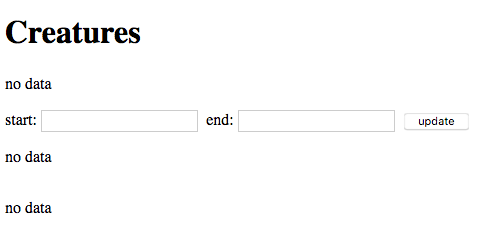
\includegraphics{../../files/capstone-first-attempt.png}

That's unexpected: we should see the initial data displayed. If we open
the console in the browser and reload the page, we see this error
message:

\begin{verbatim}
Cross-Origin Request Blocked:
The Same Origin Policy disallows reading the remote resource at http://localhost:3418/survey/stats.
(Reason: CORS header 'Access-Control-Allow-Origin' missing).
\end{verbatim}

The ``Learn More'' link given with the error message takes us to
\href{https://developer.mozilla.org/en-US/docs/Web/HTTP/CORS/Errors/CORSMissingAllowOrigin}{this
page}, which uses many science words we don't know. A web search turns
up
\href{https://en.wikipedia.org/wiki/Cross-origin_resource_sharing}{this
article on Wikipedia}, which tells us that
\protect\hyperlink{g:cors}{Cross-origin resource sharing} (CORS) is a
security mechanism. If a page loads some JavaScript, and that JavaScript
is allowed to send requests to servers other than the one that the page
came from, then villains would be able to do things like send passwords
saved in the browser to themselves. The details are too complex for this
tutorial; the good news is that they've been wrapped up in a Node
library called \texttt{cors}, which we can add to our server with just a
couple of lines of code:

\begin{verbatim}
const express = require('express')
const cors = require('cors')          // added

let dataManager = null

const app = express()
app.use(cors())                       // added

app.get('/survey/stats', (req, res, next) => {...as before...})

app.get('/survey/:start/:end', (req, res, next) => {...as before...})

app.use((req, res, next) => {...as before...})

module.exports = (dbm) => {...as before...}
\end{verbatim}

Since this code is saved in \texttt{server-1.js}, we need to create a
copy of the driver called \texttt{driver-1.js} that invokes it. Let's
run that:

\begin{verbatim}
node src/capstone/back/driver-1.js src/capstone/back/test-data.csv
\end{verbatim}

and then re-launch our application:

Second Attempt at Viewing Capstone Project

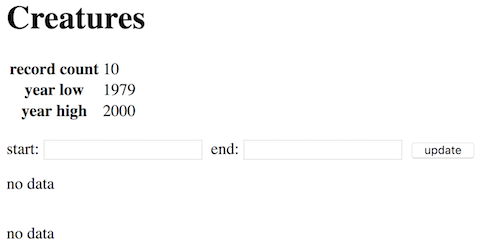
\includegraphics{../../files/capstone-second-attempt.png}

Much better! Now we can type some dates into the ``start'' and ``end''
boxes and, after we press ``update'', we get a chart and table of the
aggregated statistics for the year range given:

Completed Capstone Project

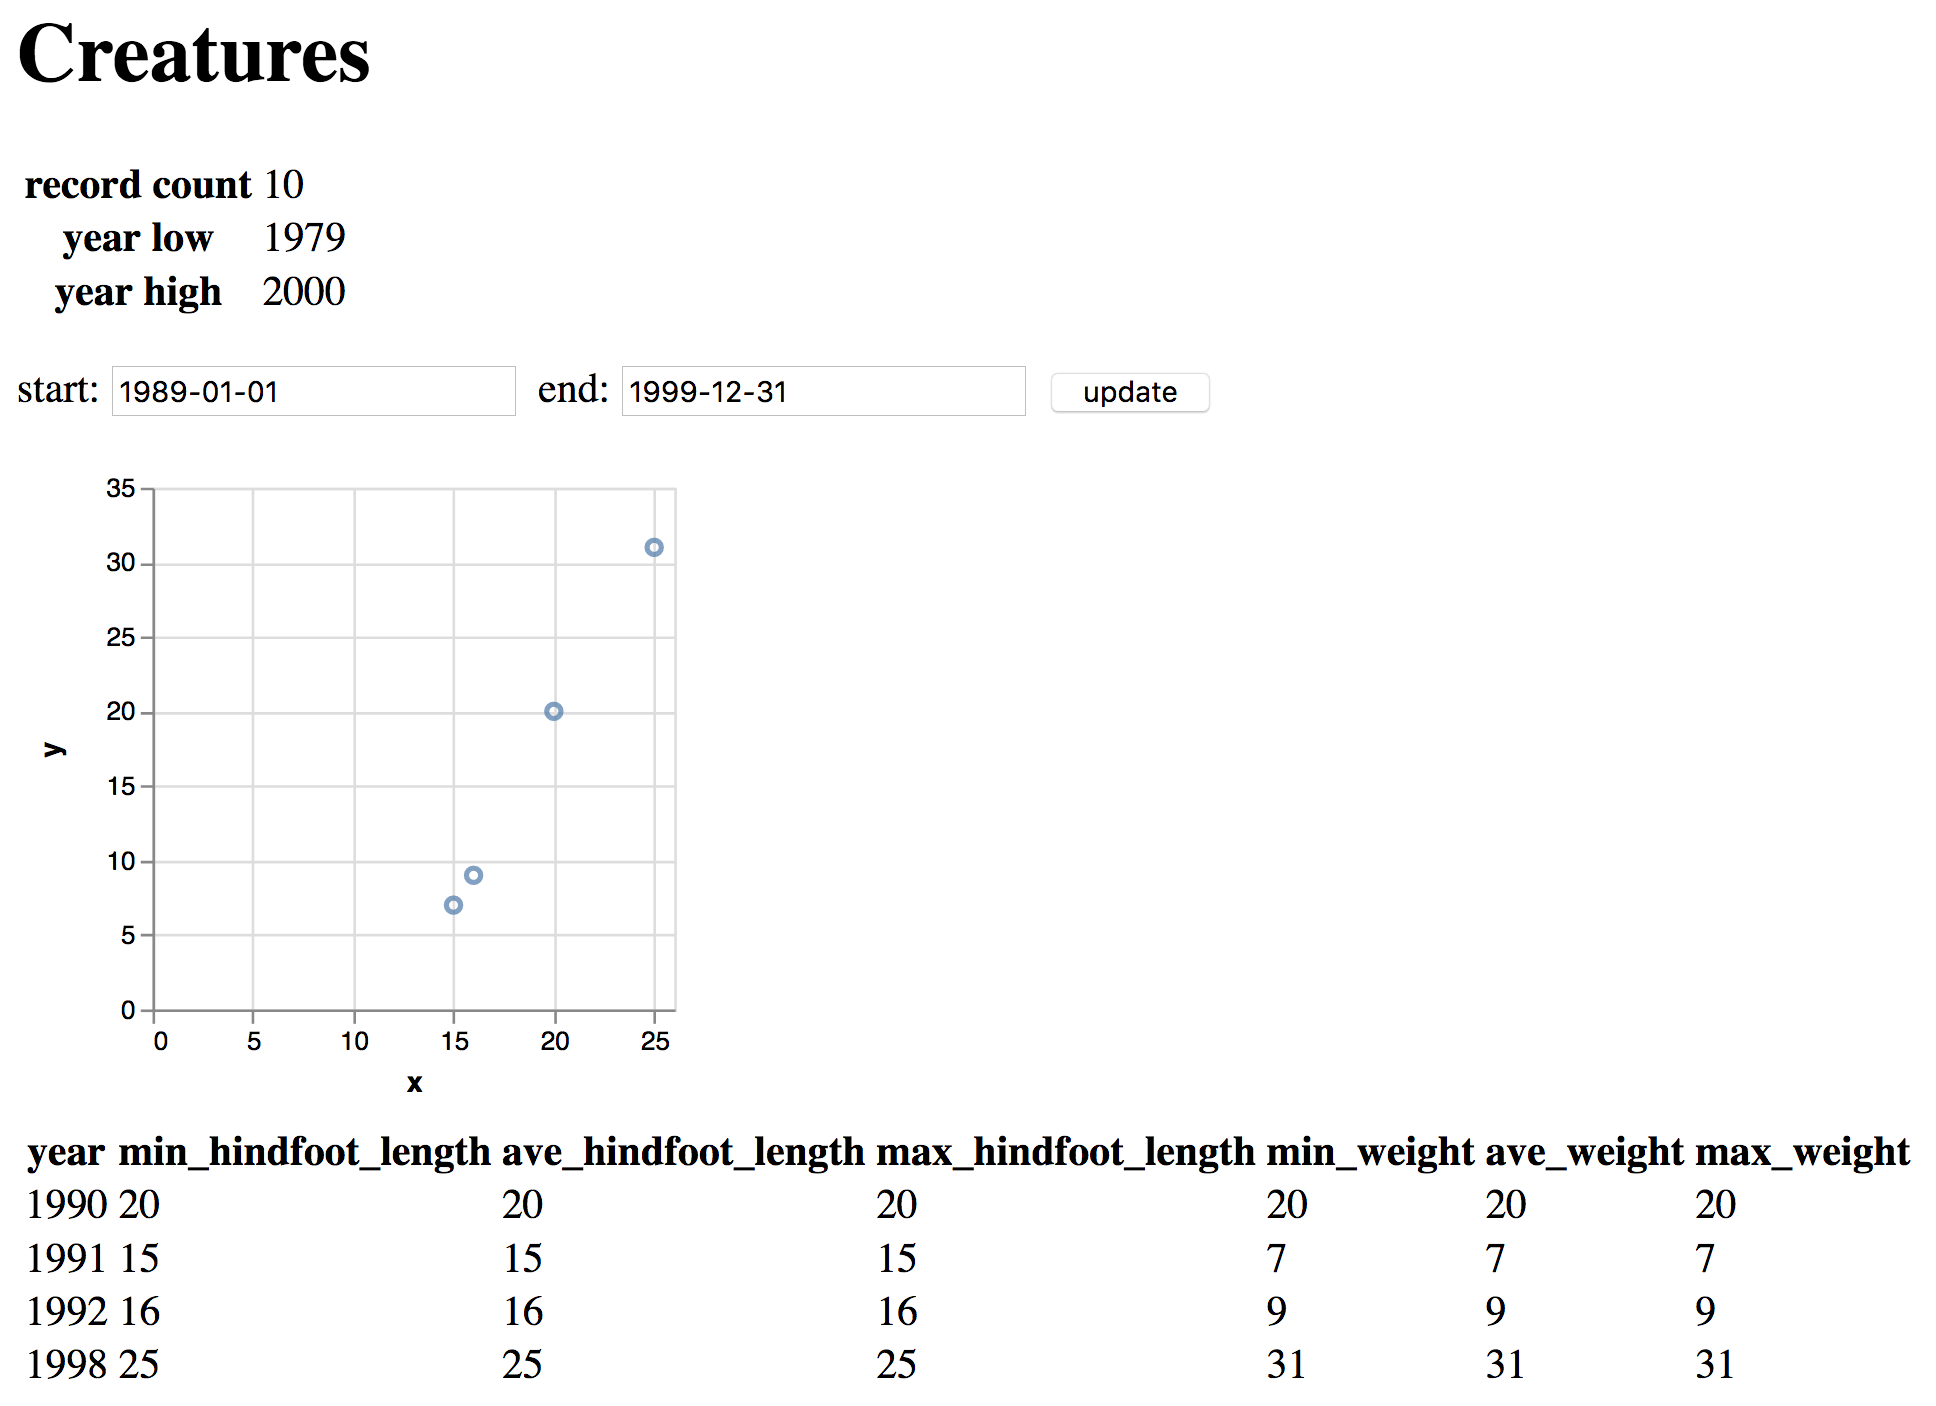
\includegraphics{../../files/capstone-complete.png}

We've built an interface, used it to submit queries that are then
handled by a server, which returns data that can be converted to content
by our React components, and our capstone project is complete.

\subsubsection{Exercises}\label{s:capstone-exercises}

\paragraph{Reporting Other Data}\label{reporting-other-data}

A user has asked for the number of male and female animals observed for
each year.

\begin{enumerate}
\tightlist
\item
  Should you add this to the existing query for yearly data or create a
  new API call?
\item
  Implement your choice.
\end{enumerate}

\paragraph{Error Checking}\label{error-checking}

\begin{enumerate}
\tightlist
\item
  Modify the server to return 400 with an error message if the range of
  years requested is invalid
\item
  Compare your implementation to someone else's. Did you define
  ``invalid'' in the same way? I.e., will your programs always return
  the same status codes for every query?
\end{enumerate}

\paragraph{Use All the Data}\label{use-all-the-data}

Create a database using all of the survey data and test the display.
What bugs or shortcomings do you notice compared to displaying test
data?

\paragraph{Merging Displays}\label{merging-displays}

The \texttt{SurveyStats} and \texttt{DataDisplay} components in the
front end both display tables.

\begin{enumerate}
\tightlist
\item
  Write a new component \texttt{TableDisplay} that will display an
  arbitrary table given a list of column names and a list of objects
  which all have (at least) those fields.
\item
  Replace \texttt{SurveyStats} and \texttt{DataDisplay} with your new
  component.
\item
  Modify your component so that it generates a unique ID for each value
  in the table. (Hint: you may need to pass in a third parameter to each
  call to serve as the root or stem of those unique IDs.)
\end{enumerate}

\paragraph{Formatting}\label{formatting}

Modify \texttt{DataDisplay} to format fractional numbers with a single
decimal place, but leave the integers as they are. Ask yourself why,
seven decades after the invention of digital computers, this isn't
easier.

\paragraph{Data, Data Everywhere}\label{data-data-everywhere}

Modify \texttt{DataChart} so that the word \texttt{data} isn't used in
so many different ways. Does doing this make you feel better about
yourself as a person? Modify it again so that the height and width of
the chart are passed in as well. Did that help?

\textbf{Key Points}

\begin{itemize}
\tightlist
\item
  Use slices of actual data to test applications.
\item
  Test summaries and small cases so that results can be checked by hand.
\item
  Store state in a class, use pure functions to display it.
\end{itemize}

\hypertarget{s:finale}{\subsection{Conclusion}\label{s:finale}}

\textbf{Questions}

\begin{itemize}
\tightlist
\item
  What have we learned?
\end{itemize}

We have come a long way since
\texttt{console.log(\textquotesingle{}hello,\ world\textquotesingle{})}
in \protect\hyperlink{s:basics}{the first lesson}. Callbacks and
promises, JSON and web servers, packaging, unit tests, and
visualization: every modern language can do them, but JavaScript is an
increasingly popular choice. Yes, it has its flaws, but if we avoid some
of its \protect\hyperlink{s:legacy}{legacy features}, it's both usable
and powerful.

Our journey doesn't stop here, though. The appendices explore some next
steps, such as \protect\hyperlink{s:logging}{logging what our server
does} and \protect\hyperlink{s:db}{using a relational database} instead
of a text file as a data store. Beyond that, you could look at more
advanced techniques in JavaScript
{[}\protect\hyperlink{Have2018}{Have2018}{]}, explore the full power of
the \href{https://d3js.org/}{D3} library for interactive visualization
{[}\protect\hyperlink{Meek2017}{Meek2017}{]}, dive into data wrangling
{[}\protect\hyperlink{Davi2018}{Davi2018}{]}, or start over completely
the way JavaScript programmers do every eight months and rewrite
everything with
\href{https://developer.mozilla.org/en-US/docs/Web/Web_Components}{Web
Components}. Whatever you do, we hope that this tutorial has helped you
get started.

Contributions of all kinds are welcome, from errata and minor
improvements to entirely new sections and chapters. Please
\href{mailto:gvwilson@third-bit.com}{email us},
\href{https://github.com/software-tools-in-javascript/js-vs-ds/issues}{file
an issue} in
\href{https://github.com/software-tools-in-javascript/js-vs-ds/}{our
GitHub repository}, or
\href{https://github.com/software-tools-in-javascript/js-vs-ds/pulls}{submit
a pull request}. Everyone whose work is incorporated will be
acknowledged. Please see \protect\hyperlink{s:contributing}{the
contributors's guide} for more information, and please note that all
contributors are required to abide by our
\protect\hyperlink{s:conduct}{Code of Conduct}.

\textbf{Key Points}

\begin{itemize}
\tightlist
\item
  We have learned a lot.
\item
  Contributions are very welcome.
\end{itemize}

\subsection{Bibliography}\label{s:bib}

\textbf{Davi2018}: Ashley Davis:
\emph{\href{https://www.manning.com/books/data-wrangling-with-javascript}{Data
Wrangling with JavaScript}}. Manning, 2018, 978-1617294846. \emph{A
step-by-step guide to managing data with JavaScript.}

\textbf{Have2018}: Martijn Haverbeke:
\emph{\href{https://eloquentjavascript.net/}{Eloquent Javascript}} (3rd
ed.). No Starch Press, 2018, 978-1593279509. \emph{The best all-around
guide to JavaScript on the market today.}

\textbf{Meek2017}: Elijah Meeks:
\emph{\href{https://www.manning.com/books/d3js-in-action-second-edition}{D3.js
in Action}} (2nd ed.). Manning, 2017, 978-1617294488. \emph{A
comprehensive guide to the D3 visualization framework.}

\textbf{Wils2018}: Greg Wilson:
\emph{\href{http://teachtogether.tech}{Teaching Tech Together}}.
Lulu.com, 2018, 978-0988113701. \emph{How to create and deliver lessons
that work and build a teaching community around them.}

\subsection{License}\label{s:license}

\emph{This is a human-readable summary of (and not a substitute for) the
license. Please see
\url{https://creativecommons.org/licenses/by/4.0/legalcode} for the full
legal text.}

This work is licensed under the Creative Commons Attribution 4.0
International license (CC-BY-4.0).

\textbf{You are free to:}

\begin{itemize}
\item
  \textbf{Share}---copy and redistribute the material in any medium or
  format
\item
  \textbf{Remix}---remix, transform, and build upon the material for any
  purpose, even commercially.
\end{itemize}

The licensor cannot revoke these freedoms as long as you follow the
license terms.

\textbf{Under the following terms:}

\begin{itemize}
\item
  \textbf{Attribution}---You must give appropriate credit, provide a
  link to the license, and indicate if changes were made. You may do so
  in any reasonable manner, but not in any way that suggests the
  licensor endorses you or your use.
\item
  \textbf{No additional restrictions}---You may not apply legal terms or
  technological measures that legally restrict others from doing
  anything the license permits.
\end{itemize}

\textbf{Notices:}

You do not have to comply with the license for elements of the material
in the public domain or where your use is permitted by an applicable
exception or limitation.

No warranties are given. The license may not give you all of the
permissions necessary for your intended use. For example, other rights
such as publicity, privacy, or moral rights may limit how you use the
material.

\hypertarget{s:conduct}{\subsection{Code of Conduct}\label{s:conduct}}

In the interest of fostering an open and welcoming environment, we as
contributors and maintainers pledge to making participation in our
project and our community a harassment-free experience for everyone,
regardless of age, body size, disability, ethnicity, gender identity and
expression, level of experience, education, socio-economic status,
nationality, personal appearance, race, religion, or sexual identity and
orientation.

\subsubsection{Our Standards}\label{s:conduct-standards}

Examples of behavior that contributes to creating a positive environment
include:

\begin{itemize}
\tightlist
\item
  using welcoming and inclusive language,
\item
  being respectful of differing viewpoints and experiences,
\item
  gracefully accepting constructive criticism,
\item
  focusing on what is best for the community, and
\item
  showing empathy towards other community members.
\end{itemize}

Examples of unacceptable behavior by participants include:

\begin{itemize}
\tightlist
\item
  the use of sexualized language or imagery and unwelcome sexual
  attention or advances,
\item
  trolling, insulting/derogatory comments, and personal or political
  attacks,
\item
  public or private harassment,
\item
  publishing others' private information, such as a physical or
  electronic address, without explicit permission, and
\item
  other conduct which could reasonably be considered inappropriate in a
  professional setting
\end{itemize}

\subsubsection{Our Responsibilities}\label{s:conduct-responsibilities}

Project maintainers are responsible for clarifying the standards of
acceptable behavior and are expected to take appropriate and fair
corrective action in response to any instances of unacceptable behavior.

Project maintainers have the right and responsibility to remove, edit,
or reject comments, commits, code, wiki edits, issues, and other
contributions that are not aligned to this Code of Conduct, or to ban
temporarily or permanently any contributor for other behaviors that they
deem inappropriate, threatening, offensive, or harmful.

\subsubsection{Scope}\label{s:conduct-scope}

This Code of Conduct applies both within project spaces and in public
spaces when an individual is representing the project or its community.
Examples of representing a project or community include using an
official project e-mail address, posting via an official social media
account, or acting as an appointed representative at an online or
offline event. Representation of a project may be further defined and
clarified by project maintainers.

\subsubsection{Enforcement}\label{s:conduct-enforcement}

Instances of abusive, harassing, or otherwise unacceptable behavior may
be reported by \href{gvwilson@third-bit.com}{emailing the project team}.
All complaints will be reviewed and investigated and will result in a
response that is deemed necessary and appropriate to the circumstances.
The project team is obligated to maintain confidentiality with regard to
the reporter of an incident. Further details of specific enforcement
policies may be posted separately.

Project maintainers who do not follow or enforce the Code of Conduct in
good faith may face temporary or permanent repercussions as determined
by other members of the project's leadership.

\subsubsection{Attribution}\label{s:conduct-attribution}

This Code of Conduct is adapted from the
\href{https://www.contributor-covenant.org}{Contributor Covenant}
version 1.4.

\subsection{Citation}\label{s:citation}

Please cite this work as:

\begin{quote}
Toby Hodges and Greg Wilson: ``JavaScript versus Data Science: A Brief
Guide for Those Who Regret That This Has Become Necessary''.
\url{https://software-tools-in-javascript.github.io/js-vs-ds/}, 2018.
\end{quote}

\hypertarget{s:contributing}{\subsection{Contributing}\label{s:contributing}}

Contributions of all kinds are welcome, from errata and minor
improvements to entirely new sections and chapters. Please
\href{mailto:gvwilson@third-bit.com}{email us},
\href{https://github.com/software-tools-in-javascript/js-vs-ds/issues}{file
an issue} in
\href{https://github.com/software-tools-in-javascript/js-vs-ds/}{our
GitHub repository}, or
\href{https://github.com/software-tools-in-javascript/js-vs-ds/pulls}{submit
a pull request}. Everyone whose work is incorporated will be
acknowledged. Please see \protect\hyperlink{s:contributing}{the
contributors's guide} for more information, and please note that all
contributors are required to abide by our
\protect\hyperlink{s:conduct}{Code of Conduct}.

\begin{itemize}
\item
  If you wish to report errata or suggest improvements to wording,
  please include the chapter name and section name (e.g.,
  \texttt{Callbacks/Anonymous\ Functions}) in the first line of the body
  of your report. Please note that we use Simplified English rather than
  Traditional English, i.e., American spelling rather than British.
\item
  If you would like to add code fragments, please put the source in
  \texttt{src/chapter/long-name.js}. Include it in a triple-backquoted
  code block of type \texttt{js}; use \texttt{sh} for shell commands and
  \texttt{text} for output (including error output). If you want to
  leave out sections of code, use \texttt{//\ ...comment...} (i.e., a
  double-slash comment and triple dots enclosing the text).
\item
  If you would like to add or fix a diagram, please edit the XML file in
  \texttt{./files/} corresponding to the chapter using
  \href{https://www.draw.io/}{draw.io}, then select the drawing and
  export as SVG with a 4-pixel boundary and transparency turned on, but
  \emph{without} including the diagram source in the exported SVG.
\item
  The \href{https://jekyllrb.com/}{Jekyll} template used in this
  tutorial can support multiple languages. We encourage translations; if
  you would like to take this on, please
  \href{mailto:gvwilson@third-bit.com}{email us}.
\end{itemize}

\subsection{Glossary}\label{s:gloss}

\textbf{absolute path}: a path that points to the same location in the
filesystem regardless of where it's evaluated. An absolute path is the
equivalent of latitude and longitude in geography. See also
\protect\hyperlink{g:relative-path}{relative path}.

\textbf{aggregation function}: a function that combines many values into
one, such as \texttt{sum} or \texttt{max}.

\textbf{anonymous function}: a function that is defined without giving
it a name, such as a callback defined where it is used. Anonymous
functions are sometimes called \emph{lambda functions} because the Greek
letter lambda is used for them in mathematics.

\textbf{argument}: see \protect\hyperlink{g:parameter}{parameter}.

\textbf{array}: a collection of values stored in a particular order and
indexed numerically. Arrays are written as comma-separated values in
square brackets, such as
\texttt{{[}\textquotesingle{}a\textquotesingle{},\ \textquotesingle{}b\textquotesingle{},\ \textquotesingle{}c\textquotesingle{}{]}}.
The term \protect\hyperlink{g:list}{list} is often used synonymously.

\textbf{ASCII}: a widely-used set of numeric codes for representing
characters from the Latin alphabet and common punctuation symbols, now
superseded by \protect\hyperlink{g:unicode}{Unicode}.

\textbf{assertion}: a statement that something is true at a certain
point in a program. Assertions are often used to define tests, but are
also used in \protect\hyperlink{g:production-code}{production code} to
check that software is behaving as it should.

\textbf{attribute}: a named property attached to an HTML
\protect\hyperlink{g:element}{element}.

\textbf{backward-compatible}: able to work consistently with older
systems.

\textbf{body} (of an HTTP message): any optional data sent after the
message's headers.

\textbf{bundler}: a tool that combines JavaScript files, web pages,
images, and other assets into a single bundle for deployment.

\textbf{cache}: a place where copies of recently-used values are stored
for quicker access.

\textbf{call stack}: a data structure that stores information about
function calls that are currently in progress. Each function call adds
another table of variable-value pairs to the top of the stack; when the
function completes, that table is discarded. See also
\protect\hyperlink{g:closure}{closure}.

\textbf{callback function}: a function A that is passed to another
function B for B to call at a later time. Callback functions are used to
implement delayed actions, such as what to do when data arrives in
response to a network request.

\textbf{Cascading Style Sheets} (CSS): a way to describe how HTML should
be rendered.

\textbf{catch}: to take responsibility for handling an
\protect\hyperlink{g:exception}{exception}. Catch is the counterpart of
\protect\hyperlink{g:throw}{throw}.

\textbf{character encoding}: a specification of how characters are
stored as bytes. The most commonly-used encoding today is
\protect\hyperlink{g:utf-8}{UTF-8}.

\textbf{child class}: a new \protect\hyperlink{g:class}{class} that
\protect\hyperlink{g:extend}{extends} an existing class (called the
\protect\hyperlink{g:parent-class}{parent class}).

\textbf{child node}: a \protect\hyperlink{g:node}{node} in a
\protect\hyperlink{g:tree}{tree} that is below some other node (which is
called the child node's \protect\hyperlink{g:parent-node}{parent}).

\textbf{class}: a programming structure that defines the properties and
behavior of a family of related \protect\hyperlink{g:object}{objects}.
Classes can \protect\hyperlink{g:inherit}{inherit} from other classes to
specify or change behavior incrementally.

\textbf{client}: a program such as a browser that sends requests to a
\protect\hyperlink{g:server}{server} and does something with the
response. It is sometimes helpful to think of clients as sorcerors
petitioning ancient gods for favors. Sometimes.

\textbf{client-side page generation}: to create an HTML page within a
\protect\hyperlink{g:client}{client} using data provided by a
\protect\hyperlink{g:server}{server}. See also
\protect\hyperlink{g:server-side-page-generation}{server-side page
generation}.

\textbf{closure}: a set of variables defined in the same
\protect\hyperlink{g:scope}{scope} whose existence has been preserved
after that scope has ended. Closures are one of the trickiest ideas in
programming.

\textbf{Comma-Separated Values} (CSV): a text format for tabular data in
which each record is one row and fields are separated by commas. There
are many minor variations, particularly around quoting of strings.

\textbf{connection manager}: an object that maintains a connection to a
database. When the code is finished working with the database, the
connection manager ensures that the connection is closed gracefully,
which helps to avoid the corruption of data.

\textbf{Content Delivery Network} (CDN): a geographically distributed
set of servers that store commonly-used or recently-used data such as
web pages so that they can be served more quickly.

\textbf{constant}: a variable whose value cannot be changed. Note that
the value itself might be changed: for example, after the statement
\texttt{const\ v\ =\ {[}\textquotesingle{}a\textquotesingle{},\ \textquotesingle{}b\textquotesingle{}{]}},
the name \texttt{v} will always refer to the same array, but the array's
contents can be changed.

\textbf{Cross-Origin Resource Sharing} (CORS): a way to control requests
made for data and other resources that aren't served by the site that
gave the browser the original page.

\textbf{declarative programming}: a style of programming in which the
user specifies what they want, and the computer figures out how to
deliver it.

\textbf{destructuring}: a form of assignment that unpacks a data
structure in one step, such as \texttt{{[}a,\ b{]}\ =\ {[}1,\ 2{]}} or
\texttt{\{left,\ right\}\ =\ \{left:\ 1,\ right:\ 2\}}.

\textbf{Domain Name System} (DNS): a decentralized naming system for
computers that translates logical names such as \texttt{third-bit.com}
into the addresses of particular computers.

\textbf{document}: an entire HTML page.

\textbf{Document Object Model} (DOM): a standard way to represent HTML
in memory. The \protect\hyperlink{g:element}{elements} and
\protect\hyperlink{g:attribute}{attributes} of the page, along with its
text, are stored as \protect\hyperlink{g:node}{nodes} organized in a
tree.

\textbf{dotted notation}: a common way to refer to the parts of
structures in programming languages. \texttt{whole.part} means ``the
thing called \texttt{part} belonging to \texttt{whole}''.

\textbf{driver}: a program that provides a standard interface through
which to communicate with another piece of hardware or software. Every
graphics card has a driver that translates generic drawing commands into
card-specific operations; every database comes with drivers that
(theoretically) allow other programs to talk to them all in the same
way.

\textbf{element}: an individual component of a web page. In HTML,
elements are enclosed in matching \texttt{\textless{}tag\textgreater{}}
and \texttt{\textless{}/tag\textgreater{}} pairs, or written as
\texttt{\textless{}tag/\textgreater{}} if they contain no content.
Elements are represented as \protect\hyperlink{g:node}{nodes} in the
\protect\hyperlink{g:dom}{DOM}.

\textbf{entry point}: a function with a known name and
\protect\hyperlink{g:signature}{signature} that a framework requires
every plugin or other dynamically-loaded content to have. The entry
point is (as the name suggests) how the framework gets into the plugin.

\textbf{escape sequence}: a sequence of characters used to represent
some other character that would otherwise have a special meaning. For
example, the escape sequence \texttt{\textbackslash{}"} is used to
represent a double-quote character inside a double-quoted string.

\textbf{event handler}: a
\protect\hyperlink{g:callback-function}{callback function} that does
something in response to a particular interaction with a browser, such
as a key being pressed or a link being clicked.

\textbf{event listener}: see \protect\hyperlink{g:event-handler}{event
handler}.

\textbf{event loop}: the fundamental processing cycle in JavaScript that
takes the next task from a list and runs it, possibly adding more tasks
to the list as it does so.

\textbf{event object}: an \protect\hyperlink{g:object}{object} that the
system passes to an \protect\hyperlink{g:event-handler}{event handler}
that contains information about the event, such as which key was
pressed.

\textbf{exception}: an object that stores information about an error or
other unusual event in a program. One part of a program will create and
\protect\hyperlink{g:throw}{throw} an exception to signal that something
unexpected has happened; another part will
\protect\hyperlink{g:catch}{catch} it.

\textbf{extend}: to create a new class from an existing class. We say
that the new class \protect\hyperlink{g:inherit}{inherits} from the old
one.

\textbf{falsy}: a horrible neologism meaning ``equivalent to false''.
See also the equally horrible \protect\hyperlink{g:truthy}{truthy}.

\textbf{fat arrow function}: a JavaScript function defined using the
syntax \texttt{(...parameters...)\ =\textgreater{}\ \{...body...\}}. Fat
arrow functions treat the special value \texttt{this} in a less
inconsistent way than their older equivalents.

\textbf{field}: a named part of a \protect\hyperlink{g:record}{record}
in a \protect\hyperlink{g:relational-database}{relational database}.
Fields are typically shown as columns in a
\protect\hyperlink{g:table}{table}.

\textbf{fixture}: the data on which a
\protect\hyperlink{g:unit-test}{unit test} is run.

\textbf{functional programming}: a style of programming in which data is
transformed through successive application of functions, rather than by
using control structures such as loops. Functional programming in
JavaScript relies heavily on
\protect\hyperlink{g:callback-function}{callbacks} and
\protect\hyperlink{g:higher-order-function}{higher-order functions}.

\textbf{global installation}: a JavaScript library placed in a location
where it can be accessed by all users and projects. See also
\protect\hyperlink{g:local-installation}{local installation}.

\textbf{global variable}: a variable defined outside any particular
function, which is therefore visible to all functions. See also
\protect\hyperlink{g:local-variable}{local variable}.

\textbf{header row}: if present, the first of a
\protect\hyperlink{g:csv}{CSV} file that defines column names (but
tragically, not their data types or units).

\textbf{heterogeneous}: having mixed type. For example, an
\protect\hyperlink{g:array}{array} is said to be heterogeneous if it
contains a mix of numbers, character strings, and values of other types.
See also \protect\hyperlink{g:homogeneous}{homogeneous}.

\textbf{higher-order function}: a function that operates on other
functions. For example, the higher-order function \texttt{forEach}
executes a given function once on each value in an
\protect\hyperlink{g:array}{array}. Higher-order functions are heavily
used in \protect\hyperlink{g:functional-programming}{functional
programming}.

\textbf{homogeneous}: having a single type. For example, an
\protect\hyperlink{g:array}{array} is said to be homogeneous if it
contains only numbers or only character strings, but not a mix of the
two.

\textbf{hostname}: the part of a URL that specifies the computer to talk
to. In \texttt{http://example.com/something/}, the hostname is
\texttt{example.com}; in \texttt{http://localhost:1234/}, it is
\texttt{localhost}.

\textbf{HTTP}: the HyperText Transfer Protocol used to exchange
information between browsers and websites, and more generally between
other \protect\hyperlink{g:client}{clients} and
\protect\hyperlink{g:server}{servers}. HTTP is a
\protect\hyperlink{g:stateless}{stateless} protocol in which
communication consists of \protect\hyperlink{g:http-request}{requests}
and \protect\hyperlink{g:http-response}{responses}.

\textbf{HTTP header}: a name-value pair at the start of an HTTP
\protect\hyperlink{g:http-request}{request} or
\protect\hyperlink{g:http-response}{response}. Headers are used to
specify what data formats the sender can handle, the date and time the
message was sent, and so on.

\textbf{HTTP method}: the verb in an
\protect\hyperlink{g:http-request}{HTTP request} that defines what the
client wants to do. Common methods are \texttt{GET} (to get data) and
\texttt{POST} (to submit data).

\textbf{HTTP request}: a precisely-formatted block of text sent from a
\protect\hyperlink{g:client}{client} (such as a browser) to a
\protect\hyperlink{g:server}{server} that specifies what resource is
being requested, what data formats the client will accept, and so on.

\textbf{HTTP response}: a precisely-formatted block of text sent from a
\protect\hyperlink{g:server}{server} back to a
\protect\hyperlink{g:client}{client} in reply to a
\protect\hyperlink{g:http-request}{request}.

\textbf{HTTP status code}: a numerical code that indicates what happened
when an \protect\hyperlink{g:http-request}{HTTP request} was processed,
such as 200 (OK), 404 (not found), or 500 (internal server error).

\textbf{in-memory database}: a database that is stored in memory rather
than in permanent storage. In-memory databases are often used for
testing.

\textbf{inherit}: to acquire properties and methods from a parent class.
See also \protect\hyperlink{g:extend}{extend}.

\textbf{internal style sheet}: a set of \protect\hyperlink{g:css}{CSS}
definitions placed inside a web page rather than in an external file.

\textbf{JSON}: a way to represent data by combining basic values like
numbers and character strings in \protect\hyperlink{g:array}{arrays} and
name/value structures. The acronym stands for ``JavaScript Object
Notation''; unlike better-defined standards like
\protect\hyperlink{g:xml}{XML}, it is unencumbered by a syntax for
comments or ways to define \protect\hyperlink{g:schema}{schemas}.

\textbf{library}: see \protect\hyperlink{g:module}{module}.

\textbf{list}: see \protect\hyperlink{g:array}{array}.

\textbf{local installation}: a JavaScript library placed inside a
particular project, and only accessible within that project. See also
\protect\hyperlink{g:global-installation}{global installation}.

\textbf{local server}: a \protect\hyperlink{g:server}{server} run on the
user's own computer, usually for testing purposes during development.

\textbf{local variable}: a variable defined inside a function which is
only visible within that function. See also
\protect\hyperlink{g:global-variable}{global variable} and
\protect\hyperlink{g:closure}{closure}.

\textbf{logging}: to record information about a program's execution in a
structured way.

\textbf{logging transport}: a channel through which
\protect\hyperlink{g:logging}{logging} messages are sent, such as
standard output (for the user's screen) or a database connection.

\textbf{member variable}: see \protect\hyperlink{g:property}{property}.

\textbf{memory diagram}: a picture showing the variables a program
contains and the data they refer to.

\textbf{method}: a function attached to an
\protect\hyperlink{g:object}{object}, typically called using
\protect\hyperlink{g:dotted-notation}{dotted notation}. In JavaScript
and many other languages, a special variable called \texttt{this} is
provided to methods to refer to the particular object for which the
method is being called.

\textbf{minimization}: to remove spaces and other extraneous characters
from source files (and possibly even rename variables). This makes those
files smaller and faster to deploy at the expense of readability.

\textbf{module}: a set of variables, functions, and/or classes grouped
together for easier management (typically but not always in a single
file). Modules are sometimes also called
\protect\hyperlink{g:library}{libraries}.

\textbf{module variable}: a variable that is visible within a module but
not outside it. See \protect\hyperlink{g:scope}{scope}.

\textbf{mutation}: changing data in place, such as modifying an element
of an array or adding a record to a database.

\textbf{name collision}: the ambiguity that arises when two or more
things in a program that have the same name are active at the same time.
The \protect\hyperlink{g:call-stack}{call stack} was invented in part to
address this problem.

\textbf{Node}: an open source implementation of JavaScript for use
outside the browser.

\textbf{node}: an in-memory representation of an element in an HTML
page. See also \protect\hyperlink{g:dom}{DOM}. Not to be confused with
\protect\hyperlink{g:node-js}{Node.js}.

\textbf{NoSQL database}: any database that doesn't use the
\protect\hyperlink{g:relational-database}{relational} model. The awkward
name comes from the fact that such databases don't use
\protect\hyperlink{g:sql}{SQL} as a query language.

\textbf{object}: a clump of variables and/or
\protect\hyperlink{g:method}{methods} grouped together in a program. In
most languages, objects can only be created as instances of
\protect\hyperlink{g:class}{classes}, but JavaScript calls anything
created using \texttt{\{...\}} an object. Do not seek to walk in the
footsteps of the sages; seek rather what they sought.

\textbf{observer-observable}: a widely-used programming pattern in which
some \protect\hyperlink{g:object}{objects} are notified and take action
when other objects change state or take action.

\textbf{override}: to replace a definition of a {[}method{]} in a
\protect\hyperlink{g:parent-class}{parent-class} with a new definition
in a \protect\hyperlink{g:child-class}{child class}.

\textbf{query parameter}: a placeholder in an
\protect\hyperlink{g:sql}{SQL} query that must be filled in with an
actual value in order for the query to run.

\textbf{package manager}: a program that does its best to keep track of
the bits and bobs of software installed on a computer. The most widely
used package manager for JavaScript is called NPM; it does its best, but
really, without proper discipline on the part of programmers, it's like
Boromir trying to hold back the orcs or a kindergarten teacher trying to
keep everyone's shirt clean during finger-painting.

\textbf{parameter}: a variable whose value is passed into a function
when the function is called. Some writers distinguish parameters (the
variables) from \protect\hyperlink{g:argument}{arguments} (the values
passed in), but others use the terms in the opposite sense. It's all
very confusing.

\textbf{parent class}: an existing \protect\hyperlink{g:class}{class}
that has been \protect\hyperlink{g:extend}{extended} to create a new
class. (The new class is called the
\protect\hyperlink{g:child-class}{child class}.)

\textbf{parent node}: the \protect\hyperlink{g:node}{node} in a
\protect\hyperlink{g:tree}{tree} that is above some other node. Every
node has a parent except the {[}root{]}\{\#root-node\}.

\textbf{parse}: to translate the text of a program or web page into a
data structure in memory that the program can then manipulate.

\textbf{polymorphism}: literally, ``having many forms''. The term refers
to the way in which \protect\hyperlink{g:object}{objects} whose
\protect\hyperlink{g:method}{methods} have the same names and
\protect\hyperlink{g:parameter}{parameters} can be used interchangeably.

\textbf{port}: a logical endpoint for communication, corresponding to a
phone number in an office building. In a URL such as
\texttt{http://example.com:8081/something}, the port is \texttt{8081}.
Only one program may use a port at any time.

\textbf{production code}: software that is delivered to an end user. The
term is used to distinguish such code from test code, deployment
infrastructure, and everything else that programmers write along the
way.

\textbf{promise}: a way to handle delayed computations in JavaScript.
Promises were supposed to make programmers' lives simpler.

\textbf{protocol}: a set of rules specifying how two things will
interact. The HTTP protocol defines the format of
\protect\hyperlink{g:http-request}{requests},
\protect\hyperlink{g:http-response}{responses}, and
\protect\hyperlink{g:http-status-code}{status codes}; a protocol for
application plugins defines how they will be referred to and what
\protect\hyperlink{g:entry-point}{entry points} they must contain.

\textbf{prototype}: an idiosyncratic mechanism used in the original
definition of JavaScript for sharing properties between objects that we
unfortunately still have to cope with.

\textbf{property}: a variable associated with an
\protect\hyperlink{g:object}{object}. The term is used to distinguish an
object's passive data from its executable
\protect\hyperlink{g:method}{methods}. Properties are sometimes called
\protect\hyperlink{g:member-variable}{member variables}.

\textbf{pseudo-random number}: a value generated in a repeatable way
that has the properties of being truly random.

\textbf{pseudo-random number generator} (PRNG): a function that can
generate a series of
\protect\hyperlink{g:pseudo-random-number}{pseudo-random numbers} after
being initialized with a \protect\hyperlink{g:seed}{seed}.

\textbf{race condition}: a situation in which the result of a
computation can vary due to operations being performed in different
orders.

\textbf{raise}: see \protect\hyperlink{g:throw}{throw}.

\textbf{read-evaluate-print loop} (REPL): an interactive program that
reads a command typed in by a user, executes it, prints the result, and
then waits patiently for the next command. REPLs are often used to
explore new ideas or for debugging.

\textbf{record}: a set of related values. In a
\protect\hyperlink{g:relational-database}{relational database}, a record
is typically shown as a single row in a
\protect\hyperlink{g:table}{table}. See also
\protect\hyperlink{g:field}{field}.

\textbf{regular expression}: a pattern for matching text.

\textbf{relational database}: a database that organizes information into
\protect\hyperlink{g:table}{tables}, each of which has a fixed set of
named \protect\hyperlink{g:field}{fields} (shown as columns) and a
variable number of \protect\hyperlink{g:record}{records} (shown as
rows). See also \protect\hyperlink{g:sql}{SQL}.

\textbf{relative path}: a path whose destination is interpreted relative
to some other location, such as the current directory. A relative path
is the equivalent of giving directions using terms like ``straight'' and
``left''. See also \protect\hyperlink{g:absolute-path}{absolute path}.

\textbf{responsive design}: an approach to building web pages and other
applications that resizes and reorganizes things smoothly for different
sizes of screens.

\textbf{RGB}: a way to represent colors as triples of red, green, and
blue intensities, each of which ranges from 0 to 255. RGB is often
augmented in modern systems to create RGBA, where the fourth component
is the pixel's transparency.

\textbf{root}: the only node in a \protect\hyperlink{g:tree}{tree} that
\emph{doesn't} have a \protect\hyperlink{g:parent-node}{parent}.

\textbf{root directory}: the directory that contains everything else,
directly or indirectly. The root directory is written \texttt{/} (a bare
forward slash).

\textbf{root element}: the \protect\hyperlink{g:element}{element} in a
document that contains every other element. The root element of a web
page is the \texttt{html} element.

\textbf{schema}: a specification of the ``shape'' of data, such as the
\protect\hyperlink{g:field}{fields} making up a database table or the
ways in which structures can be nested in
\protect\hyperlink{g:json}{JSON}.

\textbf{scope}: the portion of a program within which a definition can
be seen and used. See
\protect\hyperlink{g:global-variable}{global-variable},
\protect\hyperlink{g:local-variable}{local-variable},
\protect\hyperlink{g:module-variable}{module-variable}, and (if you are
brave) \protect\hyperlink{g:closure}{closure}.

\textbf{seed}: a value used to initialize a
\protect\hyperlink{g:prng}{pseudo-random number generator}.

\textbf{selector}: a way to identify elements within an HTML document.
The selector \texttt{h2\#contents}, for example, means ``the \texttt{h2}
element with the ID \texttt{contents}''.

\textbf{server}: a program that waits for requests from
\protect\hyperlink{g:client}{clients} and sends them data in response.
It is sometimes helpful to think of servers as harassed parents trying
to babysit a room full of unruly children.

\textbf{server-side page generation}: to create an HTML page on a
server. That HTML is then delivered as-is to a browser for display. See
also \protect\hyperlink{g:client-side-page-generation}{client-side page
generation}.

\textbf{SQL}: the language used for writing queries for
\protect\hyperlink{g:relational-database}{relational databases}. The
term was originally an acronym for Structured Query Language.

\textbf{signature}: the ordered list of argument data types required by
a function or \protect\hyperlink{g:method}{method}. If two functions or
methods have the same signature, they can be called in the same way.

\textbf{stateful}: to retain information from one operation to the next.

\textbf{stateless}: to \emph{not} retain information from one operation
to the next.

\textbf{string}: a block of text in a program. The term is short for
``character string''.

\textbf{string interpolation}: the process of inserting text
corresponding to specified values into a string, usually to make output
human-readable.

\textbf{table}: a set of uniformly-formatted
\protect\hyperlink{g:record}{records} in a
\protect\hyperlink{g:relational-database}{relational database}. Tables
are usually drawn with rows (each of which represents one record) and
columns (each of which represents a \protect\hyperlink{g:field}{field}).

\textbf{tag}: a short textual label identifying a kind of element in an
HTML page. Commonly-used tags include \texttt{p} (for a paragraph) and
\texttt{h1} (for a level-1 heading).

\textbf{template}: a document with some placeholders that can be filled
in with specific values. Templates are often used to create personalized
email messages and web pages, though their efficacy is predicated upon
relentless commercialization and devaluation of modern society's sense
of what constitutes ``personal''.

\textbf{test runner}: a program that finds and runs
\protect\hyperlink{g:unit-test}{unit tests} and reports their results.

\textbf{test suite}: a set of \protect\hyperlink{g:unit-test}{unit
tests}, usually stored in files that follow a prescribed naming
convention.

\textbf{throw}: to signal that something unexpected or unusual has
happened in a program by creating an
\protect\hyperlink{g:exception}{exception} and handing it to the
error-handling system, which then tries to find a point in the program
that will \protect\hyperlink{g:catch}{catch} it. (Some languages call
this \emph{\protect\hyperlink{g:raise}{raising}} an exception.)

\textbf{tree}: a data structure containing strictly-nested
\protect\hyperlink{g:node}{nodes}. Every node except the
\protect\hyperlink{g:root-node}{root node} must have exactly one
\protect\hyperlink{g:parent-node}{parent node}, but each node may have
zero or more \protect\hyperlink{g:child-node}{children}.

\textbf{truthy}: a truly horrible neologism meaning ``not equivalent to
false''. See also \protect\hyperlink{g:falsy}{falsy}, but only if you
are able to set aside your respect for the English language.

\textbf{Unicode}: a standard that defines numeric codes for many
thousands of characters and symbols. Unicode does \emph{not} define how
those numbers are stored; that is done by standards like
\protect\hyperlink{g:utf-8}{UTF-8}.

\textbf{unit test}: a test that exercises one property or expected
behavior of a system.

\textbf{URL} (Uniform Resource Locator): a multi-part identifier that
specifies something on a computer network. A URL may contain a protocol
(such as \texttt{http}), a hostname (such as \texttt{example.com}), a
port (such as \texttt{80}), a path (such as \texttt{/homepage.html}),
and \protect\hyperlink{g:query-parameter}{query parameters}

\textbf{UTF-8}: a way to store the numeric codes representing Unicode
characters in memory that is
\protect\hyperlink{g:backward-compatible}{backward-compatible} with the
older \protect\hyperlink{g:ascii}{ASCII} standard.

\textbf{variable}: a name in a program that has some data associated
with it. A variable's value can be changed after definition. See also
\protect\hyperlink{g:constant}{constant}.

\textbf{XML}: a set of rules for defining HTML-like tags and using them
to format documents (typically data). XML achieved license plate
popularity in the early 2000s, but its complexity led many programmers
to adopt \protect\hyperlink{g:json}{JSON} instead.

\subsection{Key Points}\label{s:keypoints}

\subsubsection{\texorpdfstring{\protect\hyperlink{s:intro}{Introduction}}{Introduction}}\label{null}

\begin{itemize}
\tightlist
\item
  Modern JavaScript is a good tool for building desktop and web-based
  applications.
\item
  This course is for people who know what loops and functions are, but
  have never used JavaScript or built web applications.
\item
  Node is a command-line interpreter for JavaScript, which can be used
  interactively or to run scripts in files.
\item
  NPM is the Node Package Manager, which can be used to find, install,
  and update libraries.
\end{itemize}

\subsubsection{\texorpdfstring{\protect\hyperlink{s:basics}{Basic
Features}}{Basic Features}}\label{null}

\begin{itemize}
\tightlist
\item
  Use \texttt{console.log} to print messages.
\item
  Use dotted notation \texttt{X.Y} to get part \texttt{Y} of object
  \texttt{X}.
\item
  Basic data types are Booleans, numbers, and character strings.
\item
  Arrays store multiple values in order.
\item
  The special values \texttt{null} and \texttt{undefined} mean `no
  value' and `does not exist'.
\item
  Define constants with \texttt{const} and variables with \texttt{let}.
\item
  \texttt{typeof} returns the type of a value.
\item
  \texttt{for\ (let\ variable\ of\ collection)\ \{...\}} iterates
  through the values in an array.
\item
  \texttt{if\ (condition)\ \{...\}\ else\ \{...\}} conditionally
  executes some code.
\item
  \texttt{false}, 0, the empty string, \texttt{null}, and
  \texttt{undefined} are false; everything else is true.
\item
  Use back quotes and \texttt{\$\{...\}} to interpolate values into
  strings.
\item
  An object is a collection of name/value pairs written in
  `\{\ldots{}\}.
\item
  \texttt{object{[}key{]}} or \texttt{object.key} gets a value from an
  object.
\item
  Functions are objects that can be assigned to variables, stored in
  lists, etc.
\item
  \texttt{function\ (...parameters...)\ \{...body...\}} is the old way
  to define a function.
\item
  \texttt{name\ =\ (...parameters...)\ =\textgreater{}\ \{...body...\}}
  is the new way to define a function.
\item
  Use \texttt{return} inside a function body to return a value at any
  point.
\item
  Use modules to divide code between multiple files for re-use.
\item
  Assign to \texttt{module.exports} to specify what a module exports.
\item
  \texttt{require(...path...)} imports a module.
\item
  Paths beginning with `.' or `/' are imported locally, but paths
  without `.' or `/' look in the library.
\end{itemize}

\subsubsection{\texorpdfstring{\protect\hyperlink{s:callbacks}{Callbacks}}{Callbacks}}\label{null}

\begin{itemize}
\tightlist
\item
  JavaScript stores the instructions making up a function in memory like
  any other object.
\item
  Function objects can be assigned to variables, put in lists, passed as
  arguments to other functions, etc.
\item
  Functions can be defined in place without ever being given a name.
\item
  A callback function is one that is passed in to another function for
  it to execute at a particular moment.
\item
  Functional programming uses higher-order functions on immutable data.
\item
  \texttt{Array.some} is true if any element in an array passes a test,
  while \texttt{Array.every} is true if they all do.
\item
  \texttt{Array.filter} selects elements of an array that pass a test.
\item
  \texttt{Array.map} creates a new array by transforming values in an
  existing one.
\item
  \texttt{Array.reduce} reduces an array to a single value.
\item
  A closure is a set of variables captured during the definition of a
  function.
\end{itemize}

\subsubsection{\texorpdfstring{\protect\hyperlink{s:oop}{Objects and
Classes}}{Objects and Classes}}\label{null}

\begin{itemize}
\tightlist
\item
  Create classes to define combinations of data and behavior.
\item
  Use the class's constructor to initialize objects.
\item
  \texttt{this} refers to the current object.
\item
  Use polymorphism to express common behavior patterns.
\item
  Extend existing classes to create new ones-sometimes.
\item
  Override methods to change or extend their behavior.
\item
  Creating extensible systems by defining interfaces and protocols.
\end{itemize}

\subsubsection{\texorpdfstring{\protect\hyperlink{s:htmlcss}{HTML and
CSS}}{HTML and CSS}}\label{null}

\begin{itemize}
\tightlist
\item
  HTML is the latest in a long line of markup languages.
\item
  HTML documents contain elements (represented by tags in angle
  brackets) and text.
\item
  Elements must be strictly nested.
\item
  Elements can contain attributes.
\item
  Use escape sequences beginning with ampersand to represent special
  characters.
\item
  Every page should have one \texttt{html} element containing a
  \texttt{head} and a \texttt{body}.
\item
  Use \texttt{\textless{}!-\/-...-\/-\textgreater{}} to include comments
  in HTML.
\item
  Use \texttt{ul} and \texttt{ol} for unordered and ordered lists, and
  \texttt{li} for list elements.
\item
  Use \texttt{table} for tables, \texttt{tr} for rows, \texttt{th} for
  headings, and \texttt{td} for regular data.
\item
  Use
  \texttt{\textless{}a\ href="..."\textgreater{}...\textless{}/a\textgreater{}}
  to create links.
\item
  Use
  \texttt{\textless{}img\ src="..."\ title="..."\ alt="..."\ /\textgreater{}}
  to include images.
\item
  Use CSS to define appearance of elements.
\item
  Use \texttt{class} and \texttt{id} to identify elements.
\item
  Use selectors to specify the elements that CSS applies to.
\end{itemize}

\subsubsection{\texorpdfstring{\protect\hyperlink{s:pages}{Manipulating
Pages}}{Manipulating Pages}}\label{null}

\begin{itemize}
\tightlist
\item
  Use a \texttt{meta} tag in a page's header to specify the page's
  character encoding.
\item
  Pages are represented in memory using a Document Object Model (DOM).
\item
  The \texttt{document} object represents the page a script is in.
\item
  Use the \texttt{querySelectorAll} method to find DOM nodes that match
  a condition.
\item
  Assign HTML text to a node's \texttt{innerHTML} property to change the
  node's content.
\item
  Use \texttt{((params)\ =\textgreater{}\ \{...\})(arguments)} to create
  and call a function in a single step.
\item
  An event listener is a function run by the browser when some specific
  event occurs.
\item
  Create an event listener for
  \texttt{\textquotesingle{}DOMContentLoaded\textquotesingle{}} to
  trigger execution of scripts \emph{after} the DOM has been
  constructed.
\item
  Check the \texttt{nodeType} or \texttt{nodeName} property of a DOM
  node to find out what kind of node it is.
\item
  Destructuring assignment allows us to assign to multiple variables by
  name in a single statement.
\item
  Use \texttt{setTimeout} to trigger execution of a function after a
  delay.
\item
  To make something run forever, have the function called by
  \texttt{setTimeout} set another timeout of the same function.
\end{itemize}

\subsubsection{\texorpdfstring{\protect\hyperlink{s:dynamic}{Dynamic
Pages}}{Dynamic Pages}}\label{null}

\begin{itemize}
\tightlist
\item
  Older dynamic web sites generated pages on the server.
\item
  Newer dynamic web sites generate pages in the client.
\item
  React is a JavaScript library for client-side page generation that
  represents HTML elements as function calls.
\item
  React replaces page elements with dynamically-generated content in
  memory (not on disk).
\item
  React functions can be customized with elements.
\item
  JSX translates HTML into React function calls so that HTML and
  JavaScript can be mixed freely.
\item
  Use Babel to translate JSX into JavaScript in the browser.
\item
  Define new React components with a pseudo-HTML element and a
  corresponding function.
\item
  Attributes to pseudo-HTML are passed to the JavaScript function as a
  \texttt{props} object.
\end{itemize}

\subsubsection{\texorpdfstring{\protect\hyperlink{s:vis}{Visualizing
Data}}{Visualizing Data}}\label{null}

\begin{itemize}
\tightlist
\item
  Vega-Lite is a simple way to build common visualizations.
\item
  Vega-Lite is declarative: the user creates a data structure describing
  what they want, and the library creates the visualization.
\item
  A Vega-List specification contains a schema identifier, a description,
  data, marks, and encodings.
\item
  The overall layout of a Vega-Lite visualization can be controlled by
  setting options.
\item
  Some applications will use \texttt{require} for server-side code and
  \texttt{import} for client-side code.
\end{itemize}

\subsubsection{\texorpdfstring{\protect\hyperlink{s:promises}{Promises}}{Promises}}\label{null}

\begin{itemize}
\tightlist
\item
  JavaScript keeps an execution queue for delayed computations.
\item
  Use promises to manage delayed computation instead of raw callbacks.
\item
  Use a callback with two arguments to handle successful completion
  (resolve) and unsuccessful completion (reject) of a promise.
\item
  Use \texttt{then} to express the next step after successful completion
  and \texttt{catch} to handle errors.
\item
  Use \texttt{Promise.all} to wait for all promises in a list to
  complete and \texttt{Promise.race} to wait for the first promise in a
  set to complete.
\item
  Use \texttt{await} to wait for the result of a computation.
\item
  Mark functions that can be waited on with \texttt{async}.
\end{itemize}

\subsubsection{\texorpdfstring{\protect\hyperlink{s:interactive}{Interactive
Sites}}{Interactive Sites}}\label{null}

\begin{itemize}
\tightlist
\item
  Define event handlers to specify what actions the browser should take
  when the user interacts with an application.
\item
  The browser passes event objects containing details of events to event
  handlers.
\item
  Use classes to keep state and event handlers together.
\item
  React calls a class's \texttt{render} to display it.
\item
  Separate models (which store data) from views (which display it).
\item
  Use \texttt{fetch} to get data from servers.
\item
  Use destructuring to get individual members from an object in a single
  step.
\item
  Modern JavaScript uses promises to manage asynchronous activities.
\end{itemize}

\subsubsection{\texorpdfstring{\protect\hyperlink{s:dataman}{Managing
Data}}{Managing Data}}\label{null}

\begin{itemize}
\tightlist
\item
  Small tabular datasets are commonly stored as Comma-Separated Values
  (CSV).
\item
  CSV can only represent regular data, and CSV files usually don't
  include units.
\item
  Nested data is commonly stored using JavaScript Object Notation
  (JSON).
\item
  JSON representations of tabular data often include redundant (and
  therefore possibly inconsistent) specifications of column names.
\item
  PapaParse is a robust CSV parsing library that produces JSON output.
\end{itemize}

\subsubsection{\texorpdfstring{\protect\hyperlink{s:server}{Creating a
Server}}{Creating a Server}}\label{null}

\begin{itemize}
\tightlist
\item
  An HTTP request or response consists of a plain-text header and an
  optional body.
\item
  HTTP is a stateless protocol.
\item
  Express provides a simple path-based JavaScript server.
\item
  Write callback functions to handle requests matching specified paths.
\item
  Provide a default handler for unrecognized requests.
\item
  Use \texttt{Content-Type} to specify the type of data being returned.
\item
  Use dynamic loading to support plugin extensions.
\end{itemize}

\subsubsection{\texorpdfstring{\protect\hyperlink{s:testing}{Testing}}{Testing}}\label{null}

\begin{itemize}
\tightlist
\item
  A unit test checks the behavior of one software component in
  isolation.
\item
  The result of a unit test can be pass, fail, or error.
\item
  Use Mocha to write and run unit tests in JavaScript.
\item
  Put assertions in unit tests to check results.
\item
  Combine tests in suites for easier management.
\item
  Divide modules into interactive and non-interactive parts for easier
  testing.
\item
  Use \texttt{supertest} to simulate interaction with a server for
  testing.
\item
  HTML is represented in memory using the Document Object Model (DOM).
\item
  Check the structure of the DOM rather than the textual representation
  of the HTML when testing.
\end{itemize}

\subsubsection{\texorpdfstring{\protect\hyperlink{s:capstone}{Capstone
Project}}{Capstone Project}}\label{null}

\begin{itemize}
\tightlist
\item
  Use slices of actual data to test applications.
\item
  Test summaries and small cases so that results can be checked by hand.
\item
  Store state in a class, use pure functions to display it.
\end{itemize}

\subsubsection{\texorpdfstring{\protect\hyperlink{s:finale}{Conclusion}}{Conclusion}}\label{null}

\begin{itemize}
\tightlist
\item
  We have learned a lot.
\item
  Contributions are very welcome.
\end{itemize}

\hypertarget{s:legacy}{\subsection{Legacy JavaScript
Issues}\label{s:legacy}}

JavaScript is now twenty-five years old, and like many
twenty-somethings, it is still struggling with issues from its
childhood. This appendix explores three of them.

\hypertarget{s:legacy-equality}{\subsubsection{Equality}\label{s:legacy-equality}}

Gary Bernhardt's
\href{https://www.destroyallsoftware.com/talks/wat}{lightning talk from
2012} may be the most-watched presentation on JavaScript ever. In it, he
rattles through some truths about the language that may surprise you:

\begin{longtable}[]{@{}lll@{}}
\toprule
Operation & Code & Result\tabularnewline
\midrule
\endhead
empty array plus empty array & \texttt{{[}{]}\ +\ {[}{]}} & \texttt{""}
(empty string)\tabularnewline
empty array plus empty object & \texttt{{[}{]}\ +\ \{\}} & \texttt{\{\}}
(empty object)\tabularnewline
empty object plus empty array & \texttt{\{\}\ +\ {[}{]}} & \texttt{0}
(number zero)\tabularnewline
empty object plus empty object & \texttt{\{\}\ +\ \{\}} & \texttt{NaN}
(not a number)\tabularnewline
\bottomrule
\end{longtable}

In order to understand this, we need to know several things (which are
laid out in more detail in
\href{https://medium.com/dailyjs/the-why-behind-the-wat-an-explanation-of-javascripts-weird-type-system-83b92879a8db}{this
article} by Abhinav Suri):

\begin{enumerate}
\tightlist
\item
  Arrays are objects whose keys happen to be sequential integers.
\item
  When JavaScript tries to add things that aren't numbers, it tries to
  convert them to numbers, and if that doesn't work, to strings (because
  it can always concatenate strings).
\item
  To convert an array to a string, JavaScript converts the elements to
  strings and concatenates them. If the array is empty, the result is an
  empty string.
\item
  When converting an object to a string, JavaScript produces
  \texttt{{[}object\ CLASS{]}}, where \texttt{CLASS} is the name of the
  object's class.
\item
  \texttt{\{\}} can be interpreted as either an empty object \emph{or}
  an empty block of code.
\end{enumerate}

So:

\begin{itemize}
\tightlist
\item
  Empty array plus empty array becomes empty string plus empty string.
\item
  Empty array plus empty object becomes empty string plus
  \texttt{{[}object\ Object{]}} (because the class of an empty object is
  just \texttt{Object}).
\item
  \texttt{\{\}\ +\ {[}{]}} is ``an empty block of code producing
  nothing, followed by \texttt{+{[}{]}}'', which becomes ``+ of the
  numeric value of the string value of an empty array'', which becomes
  ``+ of 0''.
\item
  Empty object plus empty object is interpreted as an empty object plus
  an empty block of code, and since an empty block of code doesn't
  produce a result, its ``value'' is \texttt{NaN} (not a number).
\end{itemize}

This is one of many cases in programming (and real life) where doing
something that's convenient in a simple case produces confusion in less
common cases. Every language except Canadian English has warts like
these.

\hypertarget{s:legacy-iteration}{\subsubsection{Iteration}\label{s:legacy-iteration}}

We wrote above that arrays are objects. This led to some undesirable
behavior with JavaScript's original \texttt{for} loop, which used the
word \texttt{in} rather than \texttt{of}, and which looped over all of
an object's enumerable keys:

\begin{verbatim}
const things = ['x', 'y', 'z']
things.someProperty = 'someValue'

for (let key in things) {
  console.log(key)
}
\end{verbatim}

\begin{verbatim}
0
1
2
someProperty
\end{verbatim}

That phrase ``enumerable keys'' conceals some strangeness of its own,
but in brief, a \texttt{for-in} loop will loop over keys inherited from
the object's parents as well as those defined in the object itself.
Since this is usually not what programmers want (especially for arrays),
older code often used a C-style loop:

\begin{verbatim}
for (let i = 0; i < things.length; i += 1) {
  console.log(i)
}
\end{verbatim}

\begin{verbatim}
0
1
2
\end{verbatim}

Today's solution is to use \texttt{for-of} to get the \emph{values} from
an array, which is usually what we want:

\begin{verbatim}
for (let key of things) {
  console.log(key)
}
\end{verbatim}

\begin{verbatim}
x
y
z
\end{verbatim}

Better yet, use \texttt{forEach} and take advantage of its optional
second and third arguments:

\begin{verbatim}
things.forEach((val, loc, array) => {
    console.log(`element ${loc} of ${array} is ${val}`)
})
\end{verbatim}

\begin{verbatim}
element 0 of x,y,z is x
element 1 of x,y,z is y
element 2 of x,y,z is z
\end{verbatim}

\hypertarget{s:legacy-prototypes}{\subsubsection{Prototypes}\label{s:legacy-prototypes}}

We come finally to an aspect of JavaScript that has been the cause of a
great deal of confusion: prototypes. Every JavaScript object has an
internal property called its \protect\hyperlink{g:prototype}{prototype}.
If you try to access some property of an object and it's not found,
JavaScript automatically looks in the object that the first object's
prototype refers to. If the desired property isn't there, JavaScript
looks in the prototype object's prototype, and so on.

So where do prototypes come from? If an object is created with
\texttt{new\ Something()}, and the function \texttt{Something} has a
property called \texttt{prototype}, then the new object's prototype is
set to the object to which that \texttt{prototype} property points.

This will all make sense with an example and a diagram. Let's create an
object to store the default properties of ice cream cones, then create a
function \texttt{Cone} that creates an actual cone:

\begin{verbatim}
const iceCream = {
    size: 'large'
}

const Cone = function(f) {
    this.flavor = f
}

Cone.prototype = iceCream
\end{verbatim}

We can now create a cone and look at its properties:

\begin{verbatim}
const dessert = new Cone('mustard')
console.log(`initial flavor "${dessert.flavor}" and size "${dessert.size}"`)
\end{verbatim}

\begin{verbatim}
initial flavor "mustard" and size "large"
\end{verbatim}

Prototypes

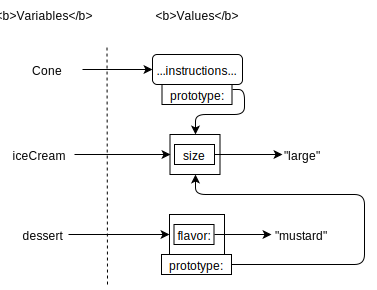
\includegraphics{../../files/legacy-prototype.svg}

If we change the \texttt{size} of our dessert, lookup finds the object's
property before looking up the chain to find the parent object's:

\begin{verbatim}
dessert.size = 'extra-large'
console.log(`modified flavor "${dessert.flavor}" and size "${dessert.size}"`)
\end{verbatim}

\begin{verbatim}
modified flavor "mustard" and size "extra-large"
\end{verbatim}

Prototypes are a way to implement inheritance for object-oriented
programming; the problem is that the mechanics are rather clumsy, and
very different from what most programmers are used to, so people built a
variety of layers on top of prototypes. To make things even more
confusing, \texttt{this} can behave in some rather odd ways, and again,
people built layers to try to insulate themselves from those oddities.
Prototypes still have their fans, but most people find modern
JavaScript's classes easier to use.

\subsection{Regular Expressions}\label{s:regexp}

A \protect\hyperlink{g:regular-expression}{regular expression} is a
pattern for matching text which is itself written as text. Alphanumeric
characters match themselves, so the regexp \texttt{/abc/} matches the
strings \texttt{"abc"} and \texttt{"some\ abc\ here"}, but not the
string \texttt{"no\ a-b-c\ here"}. Most punctuation characters have
special meaning: the character \texttt{.}, for example, matches any
single character, while \texttt{+} means ``one or more'', so
\texttt{/a.+c/} matches an `a' followed by one or more characters
followed by a `c'. Regular expressions are widely used in JavaScript,
but are outside the scope of this tutorial.

\hypertarget{s:logging}{\subsection{Logging}\label{s:logging}}

The \texttt{console.log} function we have been using is a simple form of
\protect\hyperlink{g:logging}{logging}. We can use a library called
\href{https://github.com/winstonjs/winston}{Winston} to get more control
and structure. By control, we mean that we can define levels for
messages and a threshold for the logger, and only log things that are at
least that important. This is much better than commenting and
uncommenting messages, both because it involves less typing and because
we can leave the logging code in place when we put our application into
production to debug the problems that inevitably arise after we thought
we were done. The standard error levels provided by Winston (and similar
logging libraries) are
\texttt{\textquotesingle{}error\textquotesingle{}},
\texttt{\textquotesingle{}warn\textquotesingle{}},
\texttt{\textquotesingle{}info\textquotesingle{}},
\texttt{\textquotesingle{}verbose\textquotesingle{}}, and
\texttt{\textquotesingle{}debug\textquotesingle{}}, so if we set the
threshold to \texttt{\textquotesingle{}info\textquotesingle{}}, then
\texttt{\textquotesingle{}verbose\textquotesingle{}} and
\texttt{\textquotesingle{}debug\textquotesingle{}} messages won't be
displayed.

As for structure, Winston produces log messages as JSON objects by
default so that other programs can easily read them. We can also
configure it to produce CSV, or even define some custom format, though
doing that will make everyone's life more difficult.

Whatever format we choose, we have to create and add a
\protect\hyperlink{g:logging-transport}{transport} to tell Winston where
messages should go. We will use one called \texttt{Console} that sends
messages to the screen; we can also send messages to files, to remote
logging servers, and so on. Note that we do \emph{not} create a variable
called \texttt{console} for the transport, because that will overwrite
the \texttt{console} we have been using up until now, and yes, that took
a couple of minutes to figure out\ldots{}

\begin{verbatim}
const express = require('express')
const path = require('path')
const fs = require('fs')
const winston = require('winston')

const PORT = 3418
const root = process.argv[2]
const level = process.argv[3]

const transport = new winston.transports.Console()
winston.add(transport)
winston.level = level

// Main server object.
const app = express()

// Handle all requests.
app.use((req, res, next) => {
  const actual = path.join(root, req.url)
  fs.stat(actual, (err, stats) => {
    if (err) {
      winston.error(`Unable to find "${actual}"`)
      res.status(404).send(`<html><body><p>cannot read ${actual}</p></body></html>`)
    } else if (!stats.isFile()) {
      winston.error(`"${actual}" is not a file`)
      res.status(404).send(`<html><body><p>cannot read ${actual}</p></body></html>`)
    } else {
      winston.debug(`Serving "${actual}"`)
      fs.readFile(actual, 'utf-8', (err, data) => {
    res.status(200).send(data)
      })
    }
  })
})

app.listen(PORT, () => {
  winston.info(`Running on port ${PORT} with root ${root}`)
})
\end{verbatim}

In the script above, we set the logging level with an extra command-line
parameter. If we run the script with the
\texttt{\textquotesingle{}debug\textquotesingle{}} level, all messages
appear. If we run it with the
\texttt{\textquotesingle{}info\textquotesingle{}} level, the startup
message and the 404 error messages appear, and if we run it with the
level \texttt{\textquotesingle{}error\textquotesingle{}} only the latter
appear.

\begin{verbatim}
$ node src/logging/logging-server.js src/logging/web-dir/ info
\end{verbatim}

\begin{verbatim}
{"message":"Running on port 3418 with root src/logging/web-dir/","level":"info"}
{"message":"Unable to find \"src/logging/web-dir/missing.html\"","level":"error"}
\end{verbatim}

\hypertarget{s:db}{\subsection{Using a Database}\label{s:db}}

\textbf{Questions}

\begin{itemize}
\tightlist
\item
  What options do modern applications have for storing data?
\item
  Where can I find a quick introduction to relational databases?
\item
  How can a JavaScript program get information out of a relational
  database?
\item
  How is the data returned by the database formatted?
\item
  How can I make database-backed applications testable?
\end{itemize}

Our \protect\hyperlink{s:dataman}{data manager} got information from a
single CSV file. That's fine for testing purposes, but real applications
almost always use a database of some kind. There are many options these
days for what kind, but
\protect\hyperlink{g:relational-database}{relational databases} continue
to be the workhorses of the web.

Relational databases are manipulated using a language called
\protect\hyperlink{g:sql}{SQL}, which originally stood for ``Structured
Query Language'' and is pronounced ``sequel'' or ``ess cue ell''
depending on whether the speaker is left or right handed. (Alternatives
are collectively known as \protect\hyperlink{g:nosql-database}{NoSQL
databases}, and use many different storage models.) We will use a SQL
database because it's still the most common choice, but we won't try to
introduce SQL itself: for that, see
\href{https://swcarpentry.github.io/sql-novice-survey/}{this short
tutorial}.

As an example problem, we will store information about workshops. Our
database begins with a single \protect\hyperlink{g:table}{table} with
three \protect\hyperlink{g:field}{fields} and two
\protect\hyperlink{g:record}{records}:

\begin{verbatim}
drop table if exists Workshop;

create table Workshop(
  ident         integer unique not null primary key,
  name          text unique not null,
  duration      integer not null -- duration in minutes
);

insert into Workshop values(1, "Building Community", 60);
insert into Workshop values(2, "ENIAC Programming", 150);
\end{verbatim}

In the rest of this tutorial, we will build a class to handle our
interactions with a SQLite database, test it, and then put a web service
on top of it.

\subsubsection{Starting Point}\label{s:db-start}

Our class, imaginatively named \texttt{Database}, takes the path to the
SQLite database file as a constructor parameter and creates a
\protect\hyperlink{g:connection-manager}{connection manager} through
which we can send queries and get results. We will create one method for
each query we want to run, and one helper method to display query
results. We will give all of the query methods the same
\protect\hyperlink{g:signature}{signature} so that can be handled
interchangeably. The whole thing looks like this:

\begin{verbatim}
const sqlite3 = require('sqlite3')

class Database {

  constructor (path) {
    this.db = new sqlite3.Database(path, sqlite3.OPEN_READWRITE, (err) => {
      if (err) this.fail(`Database open error ${err} for "${path}"`)
    })
  }

  getAll (args) {
    this.db.all(Q_WORKSHOP_GET_ALL, [], (err, rows) => {
      if (err) this.fail(err)
      this.display(rows)
    })
  }

  getOne (args) {
    this.db.all(Q_WORKSHOP_GET_ONE, args, (err, rows) => {
      if (err) this.fail(err)
      this.display(rows)
    })
  }

  display (rows) {
    for (let r of rows) {
      console.log(r)
    }
  }

  fail (msg) {
    console.log(msg)
    process.exit(1)
  }
}
\end{verbatim}

This makes a lot more sense once we see what the queries look like:

\begin{verbatim}
const Q_WORKSHOP_GET_ALL = `
select
  Workshop.ident        as workshopId,
  Workshop.name         as workshopName,
  Workshop.duration     as workshopDuration
from
  Workshop
`

const Q_WORKSHOP_GET_ONE = `
select
  Workshop.ident        as workshopId,
  Workshop.name         as workshopName,
  Workshop.duration     as workshopDuration
from
  Workshop
where
  Workshop.ident = ?
`
\end{verbatim}

It's easy to overlook, but the query to get details of one workshop has
a question mark \texttt{?} as the value of \texttt{Workshop.ident}. This
means that the query expects us to provide a parameter when we call it
that will be substituted in for the question mark to specify which
workshop we're interested in. This is why the arguments passed to
\texttt{getOne} as \texttt{args} are then passed through to
\texttt{db.all}; it's also why \texttt{getAll} takes an \texttt{args}
parameter, but ignores it and always passed \texttt{{[}{]}} (no extra
values) to \texttt{db.all} when running the query.

All right: what does the \protect\hyperlink{g:driver}{driver} look like?

\begin{verbatim}
function main () {
  const path = process.argv[2]
  const action = process.argv[3]
  const args = process.argv.splice(4)
  const database = new Database(path)
  database[action](args)
}

main()
\end{verbatim}

This is simple enough: it gets the path to the database file, the
desired action, and any extra arguments from \texttt{process.argv}, then
creates an instance of the \texttt{Database} class and---um. And then it
calls \texttt{database{[}action{]}(args)}, which takes a moment to
figure out. What's going on here is that an instance of a class is just
a special kind of object, and we can always look up an object's fields
by name using \texttt{object{[}name{]}}, so if the string
\texttt{action} (taken from the command-line argument) is
\texttt{getAll} or \texttt{getOne}, then
\texttt{database{[}action{]}(args)} is either
\texttt{database.getAll(args)} or
database.getOne(args)\texttt{.\ This\ is\ lever,\ but\ if\ we\ ask\ for\ an\ action\ like\ }show\texttt{\ or\ }help\texttt{\ or\ }GetOne\texttt{\ (with\ an\ upper-case\ \textquotesingle{}G\textquotesingle{}),\ then\ }database{[}action{]}`
doesn't exist and we get a very confusing error message. We really
should try to do better\ldots{}

But before then, let's try running this:

\begin{verbatim}
node database-initial.js fixture.db getAll
\end{verbatim}

\begin{verbatim}
{ workshopId: 1,
  workshopName: 'Building Community',
  workshopDuration: 60 }
{ workshopId: 2,
  workshopName: 'ENIAC Programming',
  workshopDuration: 150 }
\end{verbatim}

That seems to have worked: \texttt{getAll} was called, and the result is
an array of objects, one per record, whose names are the derived in an
obvious way from the names of the columns.

\subsubsection{In-Memory Database}\label{s:db-in-memory}

The previous example always manipulates database on disk. For testing
purposes, it's faster and safer to use an
\protect\hyperlink{g:in-memory-database}{in-memory database}. Let's
modify the constructor of \texttt{Database} to set this up:

\begin{verbatim}
  constructor (mode, path) {
    this.path = path
    switch (mode) {
    case 'memory' :
      const setup = fs.readFileSync(this.path, 'utf-8')
      this.db = new sqlite3.Database(':memory:', sqlite3.OPEN_READWRITE, (err) => {
        if (err) this.fail(`IN-MEMORY DATABASE OPEN ERROR "${err}"`)
      })
      this.db.exec(setup, (err) => {
        if (err) this.fail(`UNABLE TO INITIALIZE IN-MEMORY DATABASE FROM "${this.path}"`)
      })
      break

    case 'file' :
      this.db = new sqlite3.Database(this.path, sqlite3.OPEN_READWRITE, (err) => {
        if (err) this.fail(`DATABASE OPEN ERROR ${err} for "${path}"`)
      })
      break

    default :
      this.fail(`UNKNOWN MODE "${mode}"`)
      break
    }
  }
\end{verbatim}

If the \texttt{mode} parameter is the string \texttt{"memory"}, we
create an in-memory database and initialize it by executing a file full
of setup commands specified by the user---in our case, exactly the
commands we showed at the start of the lesson. If the \texttt{mode} is
\texttt{"file"}, we interpret the file argument as the name of an
on-disk database and proceed as before.

We put our error messages in ALL CAPS because that's the most annoying
option easily available to us. Less annoyingly, we can use destructuring
to handle command-line arguments in the driver:

\begin{verbatim}
function main () {
  const [mode, path, action, ...args] = process.argv.splice(2)
  const database = new Database(mode, path)
  database[action](args)
}
\end{verbatim}

Here, the expression \texttt{...args} means ``take anything left over
after the fixed names have been matched and put it in an array called
\texttt{args}''. With these changes in place, we can run a query to get
details of the second workshop like this:

\begin{verbatim}
node database-mode.js memory fixture.sql getOne 2
\end{verbatim}

\begin{verbatim}
{ workshopId: 2,
  workshopName: 'ENIAC Programming',
  workshopDuration: 150 }
\end{verbatim}

After a bit of experimentation, we decide to take this even further to
make testing easier. We will allow the driver to read the SQL script
itself and pass that into \texttt{Database} so that we can do the file
I/O once and then repeatedly build a database in memory for testing.
That way, each of our tests will start with the database in a known,
predictable state, regardless of what other tests may have run before
and what changes they might have made to the database. Here are the
changes to the constructor:

\begin{verbatim}
  constructor (mode, arg) {
    switch (mode) {
      case 'direct' :
        this._inMemory(arg)
        break

      case 'memory' :
        const setup = fs.readFileSync(arg, 'utf-8')
        this._inMemory(setup)
        break

      case 'file' :
        this._inFile(arg)
        break

      default :
        this.fail(`Unknown mode "${mode}"`)
        break
    }
  }
\end{verbatim}

And here are the supporting methods:

\begin{verbatim}
  _inMemory (script) {
    this.db = new sqlite3.Database(':memory:', sqlite3.OPEN_READWRITE, (err) => {
      if (err) this.fail(`In-memory database open error "${err}"`)
    })
    this.db.exec(script, (err) => {
      if (err) this.fail(`Unable to initialize in-memory database from "${script}"`)
    })
  }

  _inFile (path) {
    this.db = new sqlite3.Database(path, sqlite3.OPEN_READWRITE, (err) => {
      if (err) this.fail(`Database open error "${err}" for "${path}"`)
    })
  }
\end{verbatim}

We also need to change the driver (and check, finally, that the
requested action is actually supported):

\begin{verbatim}
function main () {
  let [mode, setup, action, ...args] = process.argv.splice(2)
  if (mode === 'direct') {
    setup = fs.readFileSync(setup, 'utf-8')
  }
  const database = new Database(mode, setup)
  if (!(action in database)) {
    database.fail(`No such operation "${action}"`)
  }
  database[action](args)
}
\end{verbatim}

\subsubsection{Making It Testable}\label{s:db-testable}

We put the database class and its driver in separate files so that
applications can load just the former. We will now change the database
query methods to return results for display rather than displaying them
directly, since we will eventually want to compare them or return them
to a server rather than printing them:

\begin{verbatim}
class Database {

  // ...as before...

  getAll (args) {
    this.db.all(Q_WORKSHOP_GET_ALL, [], (err, rows) => {
      if (err) this.fail(err)
      return rows
    })
  }

  // ...as before...
}
\end{verbatim}

The driver then looks like this:

\begin{verbatim}
const Database = require('./separate-database')

const display = (rows) => {
  for (let r of rows) {
    console.log(r)
  }
}

const main = () => {
  let [mode, path, action, ...args] = process.argv.splice(2)
  const db = new Database(mode, path)
  if (!(action in db)) {
    db.fail(`No such operation "${action}"`)
  }
  const result = db[action](args)
  display(result)
}

main()
\end{verbatim}

Let's try running it:

\begin{verbatim}
node separate-driver.js file fixture.db getAll
\end{verbatim}

\begin{verbatim}
  for (let r of rows) {
              ^

TypeError: Cannot read property 'Symbol(Symbol.iterator)' of undefined
    at display (/project/src/db/separate-driver.js:4:15)
    at main (/project/src/db/separate-driver.js:16:3)
\end{verbatim}

Whoops: the \texttt{run} method of the database delivers results to a
callback; its own result is therefore \texttt{undefined}, so there's
nothing in the caller to print.

The solution is to give the \texttt{get} methods a callback of their
own:

\begin{verbatim}
class Database {

  // ...as before...

  getAll (callback, args) {
    this.db.all(Q_WORKSHOP_GET_ALL, [], (err, rows) => {
      if (err) this.fail(err)
      callback(rows)
    })
  }

  // ...as before...
}
\end{verbatim}

We then change the driver to pass \texttt{display} to the database
method it's calling:

\begin{verbatim}
const Database = require('./callback-database')

const display = (rows) => {
  for (let r of rows) {
    console.log(r)
  }
}

const main = () => {
  let [mode, path, action, ...args] = process.argv.splice(2)
  const db = new Database(mode, path)
  if (!(action in db)) {
    db.fail(`No such operation "${action}"`)
  }
  db[action](display, args)
}

main()
\end{verbatim}

This looks strange the first few (dozen) times, but it's the way
JavaScript works: instead of asking for something and then operating on
it, we say, ``Here's what we want to do once results are available.''

\subsubsection{Testing}\label{s:db-testing}

We can finally write some tests:

\begin{verbatim}
const assert = require('assert')
const Database = require('./callback-database')

const FIXTURE = `
drop table if exists Workshop;

create table Workshop(
  ident           integer unique not null primary key,
  name            text unique not null,
  duration        integer not null -- duration in minutes
);

insert into Workshop values(1, "Building Community", 60);
insert into Workshop values(2, "ENIAC Programming", 150);
`

describe('database', () => {

  it('should return all workshops', (done) => {
    expected = [
      { workshopName: 'Building Community', workshopDuration: 60, workshopId: 1 },
      { workshopName: 'ENIAC Programming', workshopDuration: 150, workshopId: 2 }
    ]
    new Database('direct', FIXTURE).getAll([], (results) => {
      assert.deepEqual(results, expected, 'Got expected workshops')
      done()
    })
  })

  it('should return one workshop', (done) => {
    expected = [
      { workshopName: 'Building Community', workshopDuration: 60, workshopId: 1 }
    ]
    new Database('direct', FIXTURE).getOne(1, (results) => {
      assert.deepEqual(results, expected, 'Got single expected workshop')
      done()
    })
  })

  it('can only get workshops that exist', (done) => {
    new Database('direct', FIXTURE).getOne(99, (results) => {
      assert.deepEqual(results, [], 'Got no workshops matching nonexistent key')
      done()
    })
  })

})
\end{verbatim}

Each test has the same structure: we define the expected result, create
an entirely new database in memory, and then call the method being
tested, passing it the fixture and the callback that will receives
results. That callback uses \texttt{assert} to check results and
\texttt{done} to signal that the test has completed.

\subsubsection{Updating the Database}\label{s:db-mutate}

The \protect\hyperlink{s:dataman}{data manager we built earlier} only
let us read data; we couldn't modify it. Let's add a bit more to our
database class to support \protect\hyperlink{g:mutation}{mutation}:

\begin{verbatim}
// ...imports as before...

const Q_WORKSHOP_GET_ALL = // ...as before...
const Q_WORKSHOP_GET_ONE = // ...as before...

const Q_WORKSHOP_ADD = `
insert into Workshop(name, duration) values(?, ?);
`

const Q_WORKSHOP_DELETE = `
delete from Workshop where ident = ?;
`

class Database {

  constructor (mode, arg) {
    // ...as before...
  }
  getAll (args, callback) {
    // ...as before...
  }
  getOne (args, callback) {
    // ...as before...
  }

  addOne (args, callback) {
    this.db.run(Q_WORKSHOP_ADD, args, function (err, rows) {
      if (err) this.fail(err)
      callback([], this.lastID)
    })
  }

  deleteOne (args, callback) {
    this.db.run(Q_WORKSHOP_DELETE, args, (err, rows) => {
      if (err) this.fail(err)
      callback([], undefined)
    })
  }

  fail (msg) {
    // ...as before...
  }
  _inMemory (script) {
    // ...as before...
  }
  _inFile (path) {
    // ...as before...
  }
}

module.exports = Database
\end{verbatim}

The additions are straightforward: the query that does the work is
passed to \texttt{this.db.run} along with the incoming arguments that
specify what is to be added or deleted, and an empty list of rows is
passed to the action callback (since adding and deleting don't return
anything). Testing involves a little more typing, since want to check
that the database is in the right state after the operation:

\begin{verbatim}
// ...imports as before...

const FIXTURE = // ...as before...

describe('mutating database', () => {

  it('can add a workshop', (done) => {
    const duration = 35, name = 'Creating Bugs'
    const db = new Database('direct', FIXTURE)
    db.addOne([name, duration], function (results, lastID) {
      assert.deepEqual(results, [], 'Got empty list as result when adding')
      assert.equal(lastID, 3, 'Got the correct last ID after adding')
      db.getAll([], (results) => {
        expected = [
          { workshopName: 'Building Community', workshopDuration: 60, workshopId: 1 },
          { workshopName: 'ENIAC Programming', workshopDuration: 150, workshopId: 2 },
          { workshopName: name, workshopDuration: duration, workshopId: 3 }
        ]
        assert.deepEqual(results, expected, 'Got expected workshops after add')
        done()
      })
    })
  })

  it('can delete a workshop', (done) => {
    const db = new Database('direct', FIXTURE)
    db.deleteOne([1], (results, lastID) => {
      assert.equal(lastID, undefined, 'Expected last ID to be undefined')
      assert.deepEqual(results, [], 'Got empty list as result when deleting')
      db.getAll([], (results) => {
        expected = [
          { workshopName: 'ENIAC Programming', workshopDuration: 150, workshopId: 2 }
        ]
        assert.deepEqual(results, expected, 'Got expected workshops after delete')
        done()
      })
    })
  })
})
\end{verbatim}

\subsubsection{Exercises}\label{s:db-exercises}

\paragraph{Copying Records}\label{copying-records}

Write a program that copies all the rows from the table
\texttt{Workshop} in a database \texttt{source.db} to a table with the
same name in a new database \texttt{backup.db}.

\paragraph{Filtering Records}\label{filtering-records}

Add a new method to the \texttt{Database} class to get all workshops
that are longer than a specified time:

\begin{verbatim}
const db = new Database(path)
const rows = db.getLongerThan(100)
assert.deepEqual(rows, [
  {workshopName: 'ENIAC Programming', workshopDuration: 150, workshopId: 2}
])
\end{verbatim}

Your \texttt{Database.getLongerThan} method's SQL query will need to use
a \texttt{where} clause that selects specific records.

\paragraph{More Filtering}\label{more-filtering}

The SQL query encapsulated in the variable below can be used to find all
workshop whose duration falls within a range.

\begin{verbatim}
const Q_WORKSHOP_DURATION_RANGE = `
select
  Workshop.ident        as workshopId,
  Workshop.name         as workshopName,
  Workshop.duration     as workshopDuration
from
  Workshop
where
  (Workshop.duration <= ?) and (Workshop.duration >= ?)
`
\end{verbatim}

What do the \texttt{?}s mean in this query? Write another method for the
\texttt{Database} class called \texttt{getWithinLengthRange({[}args{]})}
that uses this query, taking arguments from the commandline as before.
What happens when you provide the wrong number of arguments to this
function? Or if you provide them in the wrong order? Can you write a
test that provides more useful feedback than this?

\paragraph{Handling Errors}\label{handling-errors}

The \texttt{Database} class prints a message and exits when it detects
an error. This is bad practice, and I should be ashamed of having done
it. The right thing to do is to \protect\hyperlink{g:throw}{throw} an
\protect\hyperlink{g:exception}{exception} that main program can
\protect\hyperlink{g:catch}{catch} and handle however it wants.

\begin{enumerate}
\tightlist
\item
  Modify the code to do this.
\item
  Modify the tests to check that the right exceptions are thrown when
  they should be.
\end{enumerate}

\paragraph{Using a Database with a
Server}\label{using-a-database-with-a-server}

Rewrite the \protect\hyperlink{s:capstone}{capstone project} to use a
database instead of a file for data storage.

\textbf{Key Points}

\begin{itemize}
\tightlist
\item
  Relational databases store data in tables made up of fields (columns)
  and records (rows).
\item
  Programs interact with relational databases using SQL queries.
\item
  Non-relational databases store data as JSON-like data structures.
\item
  Basic SQL queries select and filter data.
\item
  JavaScript programs send SQL queries to a database and get the results
  as a list of lists.
\item
  Using an in-memory database to make tests faster and ensure that they
  are isolated.
\item
  Use callbacks to handle the results of queries.
\end{itemize}

\subsection{Extensible Servers}\label{s:extensible}

\textbf{Questions}

\begin{itemize}
\tightlist
\item
  How can I extend a server without rewriting it?
\end{itemize}

Suppose we want to extend our \protect\hyperlink{s:server}{server} in
some way. We could edit the source file and add some more URL handlers,
or we could have it load JavaScript dynamically and run that.

\begin{verbatim}
const express = require('express')

const PORT = 3418

// Main server object.
const app = express()

// Handle all requests.
app.use((req, res, next) => {
  if (req.url.endsWith('.js')) {
    const libName = './'.concat(req.url.slice(0, -3))
    const dynamic = require(libName)
    const data = dynamic.page()
    res.status(200).send(data)
  }

  else {
    res.status(404).send(`<html><body><p>"${req.url}" not found</p></body></html>`)
  }
})

app.listen(PORT, () => { console.log(`listening on port ${PORT}...`) })
\end{verbatim}

This simple server checks whether the path specified in the URL ends
with \texttt{.js}. If so, it constructs something that looks like the
name of a library by stripping off the \texttt{.js} and prefixing the
stem with \texttt{./}, then uses \texttt{require} to load that file.
Assuming the load is successful, it then calls the \texttt{page}
function defined in that file. We can create a very simple plugin like
this:

\begin{verbatim}
function page() {
  return ('<html><body><h1>Plugin Content</h1></body></html>');
}

module.exports = {
  page: page
}
\end{verbatim}

If we run the server:

\begin{verbatim}
node src/extensible/dynamic.js
\end{verbatim}

and then go to \texttt{http://localhost:4000/plugin.js}, we get back a
page containing the title ``Plugin Content''.

This is an example of a very powerful technique. Rather than building
everything into one program, we can provide a
\protect\hyperlink{g:protocol}{protocol} for plugins so that people can
add new functionality without rewriting what's already there. Each
plugin must have an \protect\hyperlink{g:entry-point}{entry point} like
the function \texttt{page} so that the framework knows where to start.

\textbf{Key Points}

\begin{itemize}
\tightlist
\item
  Servers (and other programs) can dynamically load modules to extend
  their capabilities.
\item
  Dynamically loading modules is a security risk.
\end{itemize}
